\documentclass[11pt]{article}
%----------------------------------------------------------------------------------------
%	Paquetes y configuraciones
%----------------------------------------------------------------------------------------
% \usepackage[numbers]{natbib}
% \bibliographystyle{apalike}

\usepackage{amsfonts}
\usepackage{amsmath}
\usepackage{amssymb,amsthm}
\usepackage{enumerate}
\usepackage{enumitem}
\usepackage[utf8]{inputenc}
\usepackage[T1]{fontenc}
\usepackage{geometry}
\usepackage{hyperref}
\geometry{left=1.75cm,right=1.75cm,top=2.5cm,bottom=2.5cm}
\usepackage{caption}
\usepackage{subcaption}

\usepackage{url}
\def\UrlBreaks{\do\/\do-}
\usepackage{multirow}
\usepackage{multicol}
\usepackage{enumitem}
\usepackage{nicefrac}
\usepackage{graphicx}
\usepackage{stmaryrd}
\usepackage{dsfont}
\usepackage{bropd}
\usepackage{easybmat}
\usepackage{setspace}
\usepackage{comment}
\usepackage{mathpazo}
\usepackage{array}
\usepackage{commath}
\usepackage{xcolor}
\usepackage{placeins}

\usepackage{sectsty}
\sectionfont{\centering\selectfont}
% \subsectionfont{\centering\fontsize{10}{10}\selectfont\scshape}

\usepackage{doi}
\usepackage[backend=biber,style=ieee,sorting=none,citestyle=numeric,maxbibnames=3,doi=true]{biblatex}
\addbibresource{literature.bib}

\newtheorem{theorem}{Theorem}[section]
\newtheorem{corollary}{Corollary}[theorem]
\newtheorem{proposition}{Proposition}[theorem]
\newtheorem{lemma}[theorem]{Lemma}
\newtheorem{definition}[theorem]{Definition}
\newtheorem{remark}[theorem]{Remark}
\newtheorem{example}[theorem]{Example}
\newtheorem{claim}{Claim}[subsection]


\usepackage{siunitx} % for units

\usepackage[font=small]{caption}
\usepackage[font=small]{subcaption}
\captionsetup{subrefformat=parens}
\usepackage{booktabs} % nice headers for tables


\newcommand{\R}{\mathbb{R}}
\newcommand{\Z}{\mathbb{Z}}
\newcommand{\N}{\mathbb{N}}
\newcommand{\CC}{\mathcal{C}}
\newcommand{\llb}{\llbracket}
\newcommand{\rrb}{\rrbracket}
\newcommand{\by}{\mathbf{y}}
\newcommand{\bv}{\mathbf{v}}

\DeclareMathOperator{\dom}{dom}
\DeclareMathOperator{\dist}{dist}
\DeclareMathOperator{\supp}{supp}
\setcounter{MaxMatrixCols}{20}


\SetLabelAlign{parright}{\parbox[t]{\labelwidth}{\raggedright#1}}
\allowdisplaybreaks





\usepackage[symbol,hang,flushmargin]{footmisc}

\renewcommand{\thefootnote}{\fnsymbol{footnote}}


\linespread{1.38}

%---------------------------------------- Autoría ---------------------------------------- %
%\usepackage{titling}
%\predate{}
%\postdate{\vspace{-2\baselineskip}}



\title{\bf
    \Large
    Defining Good Neighbours: Modelling Root Traits for Beneficial Plant-Plant Interactions
}
\author{
    Karolína Benková, Liz Howell, Andrés Miniguano Trujillo\footnote{ \texttt{\{K.Benkova, L.Howell, Andres.Miniguano-Trujillo\}@ed.ac.uk} }
}
\date{}



\begin{document}
%\pagenumbering{Roman} 
% \maketitle
\begin{titlepage}
    \begin{center}
        \vspace*{2cm}
        
        \Huge
        \textbf{Defining Good Neighbours: Modelling Root Traits for Beneficial Plant-Plant Interactions}
        
            
        \vspace{1cm}
        
        \Large Karolína Benková, Liz Howell, Andrés Miniguano Trujillo\footnote{\normalsize Maxwell Institute for Mathematical Sciences,   \texttt{\{K.Benkova,Liz.Howell,Andres.Miniguano-Trujillo\}@ed.ac.uk}}
        
            
        \vspace{1.5cm}
            
        \Large
        Supervised by Dr Mariya Ptashnyk\footnote{\normalsize Heriot-Watt University, \texttt{M.Ptashnyk@hw.ac.uk}} \\ 
        In collaboration with Dr Tim George\footnote{\normalsize The James Hutton Institute, \texttt{\{Tim.George,Ali.Karley\}@hutton.ac.uk}} and Dr Alison Karley\textsuperscript{\small\ddag}

        \vfill
            
        
    \end{center}
\end{titlepage}
\newpage
\pagenumbering{roman}

\section*{Executive summary}
"Please can you include a <1 page executive
summary, aimed at the industrial partner.  This should include a summary
of the problem, methods used, analysis, conclusions, recommendations,
and any critical analysis (i.e. limitations) of the report/results.
Please put this at the start of your report (preferably right before the
'academic' abstract)."

% You can (obviously) find some information and guidance on the web. Some
% possible places to start are:

% https://en.wikipedia.org/wiki/Executive_summary
% https://unilearning.uow.edu.au/report/4bi1.html
% https://hbswk.hbs.edu/archive/crafting-a-powerful-executive-summary

\newpage
\section*{Abstract}
\newpage
\doublespacing
\tableofcontents

\singlespacing
\newpage
\pagenumbering{arabic}
\setcounter{page}{1}


%%%%%%%%%%%%%%%%%%%%%%%%%%%%%%%%%%%%%%%%%%%%%%%%%%%
% \section{Zinc uptake by rice through phytosiderophore secretion}

%%%%%%%%%%%%%%%%%
%%%%%%%%%%%%%%%%%

\section{Biological Background}

\subsection{Motivation}
Nutrient deficiency is one of the most prolific problems affecting crops in the modern age. In particular, humans rely upon grasses and grains to introduce zinc ($Zn$) and other key nutrients to our diets. Thus, as our population grows, we would like to plant more crops to feed ourselves and, as we take up more space on the Earth, we would look to grow those plants in increasingly hostile environments. Indeed,  many of the elements that make up the fertilisers we use the most to improve soil conditions are difficult to obtain or process. One of the mechanisms we can use to address this is intercropping, the practice of mixing the species or genotypes of species as we plant. This can occur in time, through crop rotation which is the practice of planting different crops each season to improve soil condition. For example many farmers rotate planting a four crop system of brassicas, legumes, onions, and potato plants to increase soil nutrients and ensure that certain plant-focused soil pests will die out year by year. Intercropping can also occur in space, through the practice of planting different species of plants in proximity to one another to encourage a mutually beneficial relationship between them. This paper will explore the benefits of intercropping different genotypes and species of grass plants to consider the benefits this may have upon nutrient uptake within their root systems.

One of the main nutrients plants rely upon is phosphorus ($P$) which is used in important processes such as cell membrane construction. It is therefore important to maximise plant production of new cells and leaf growth such that there is a ready supply of $P$ available in the soil. For this reason, many commercial farming programs rely on $P$ fertilisers produced from either acid- or heat-treated rock phosphate. This rock phosphate is mined primarily in countries such as Morocco, China and Russia, each of which has their own political difficulties when it comes to obtaining a steady supply of resources. Thus, if plants can be bred or inter-cropped in a certain way to more efficiently access and use the $P$ compounds present in soil without the need of supplying the soil with additional source of $P$, this would be of great benefit to many farming and crop focused industries.

In this project, we will reproduce the model of zinc uptake by rice using metal-complexing phytoside\-rophore as an exudate \cite{Ptashnyk-2011} and extend it to model interaction of roots of two different plants growing next to each other (i.e. intercropped) with two different exudates and one common nutrient being taken from the soil. The parameters we choose to use in the model correspond to barley and tobacco plants which secrete citrate and phytase so that the plant can access $P$ from the soil in the form of phosphate. We will also experiment with different parameter set-ups and report on findings regarding the combinations of parameter values or plant traits that enhance phosphate uptake. The findings about what traits are beneficial for nutrient uptake in intercropping might be especially useful for farming focused industries as the results are not limited only to hypothetical barley and tobacco system but to any combination of plants which might satisfy the characteristics we propose. 

\begin{figure}[!htb]
  \vspace{-1cm}
     \centering
     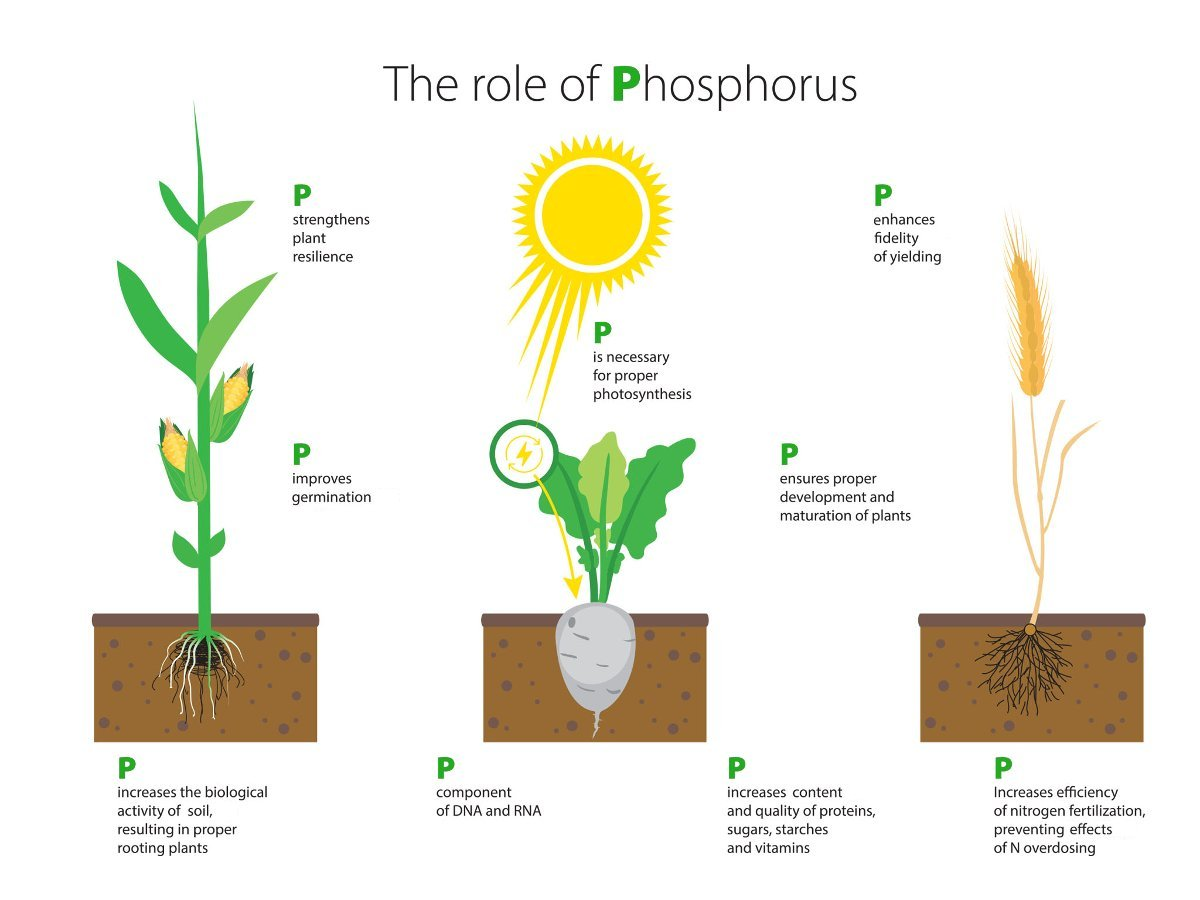
\includegraphics[width=0.7\textwidth]{Phosphorus-plant-roles.jpg}
     \caption{Different roles of phosphorus in plant systems.}
     \label{fig:Phos}
 \end{figure}
 
\subsection{Dynamics at the root}
Now that we have established some motivation to this project, let us introduce a plant system we are going to be working with. First, we will briefly explain how plant roots interact with the soil around them in order to gather nutrients, and then we will consider the work in \cite{Ptashnyk-2011} to model this process mathematically.
 

\subsubsection{Root exudation and absorption}
When a plant sprouts from a seed, it puts roots out into the soil below it. For many plants, the growth of the roots results in a large system of roots. This system can contain one characteristic (or larger) primary root which is surrounded by many secondary roots and root hairs. The growth of the root hairs can be affected by the soil environment in which the plant is growing, see Fig. \ref{fig:roots}.

% \begin{figure}{h}
%     \centering
%     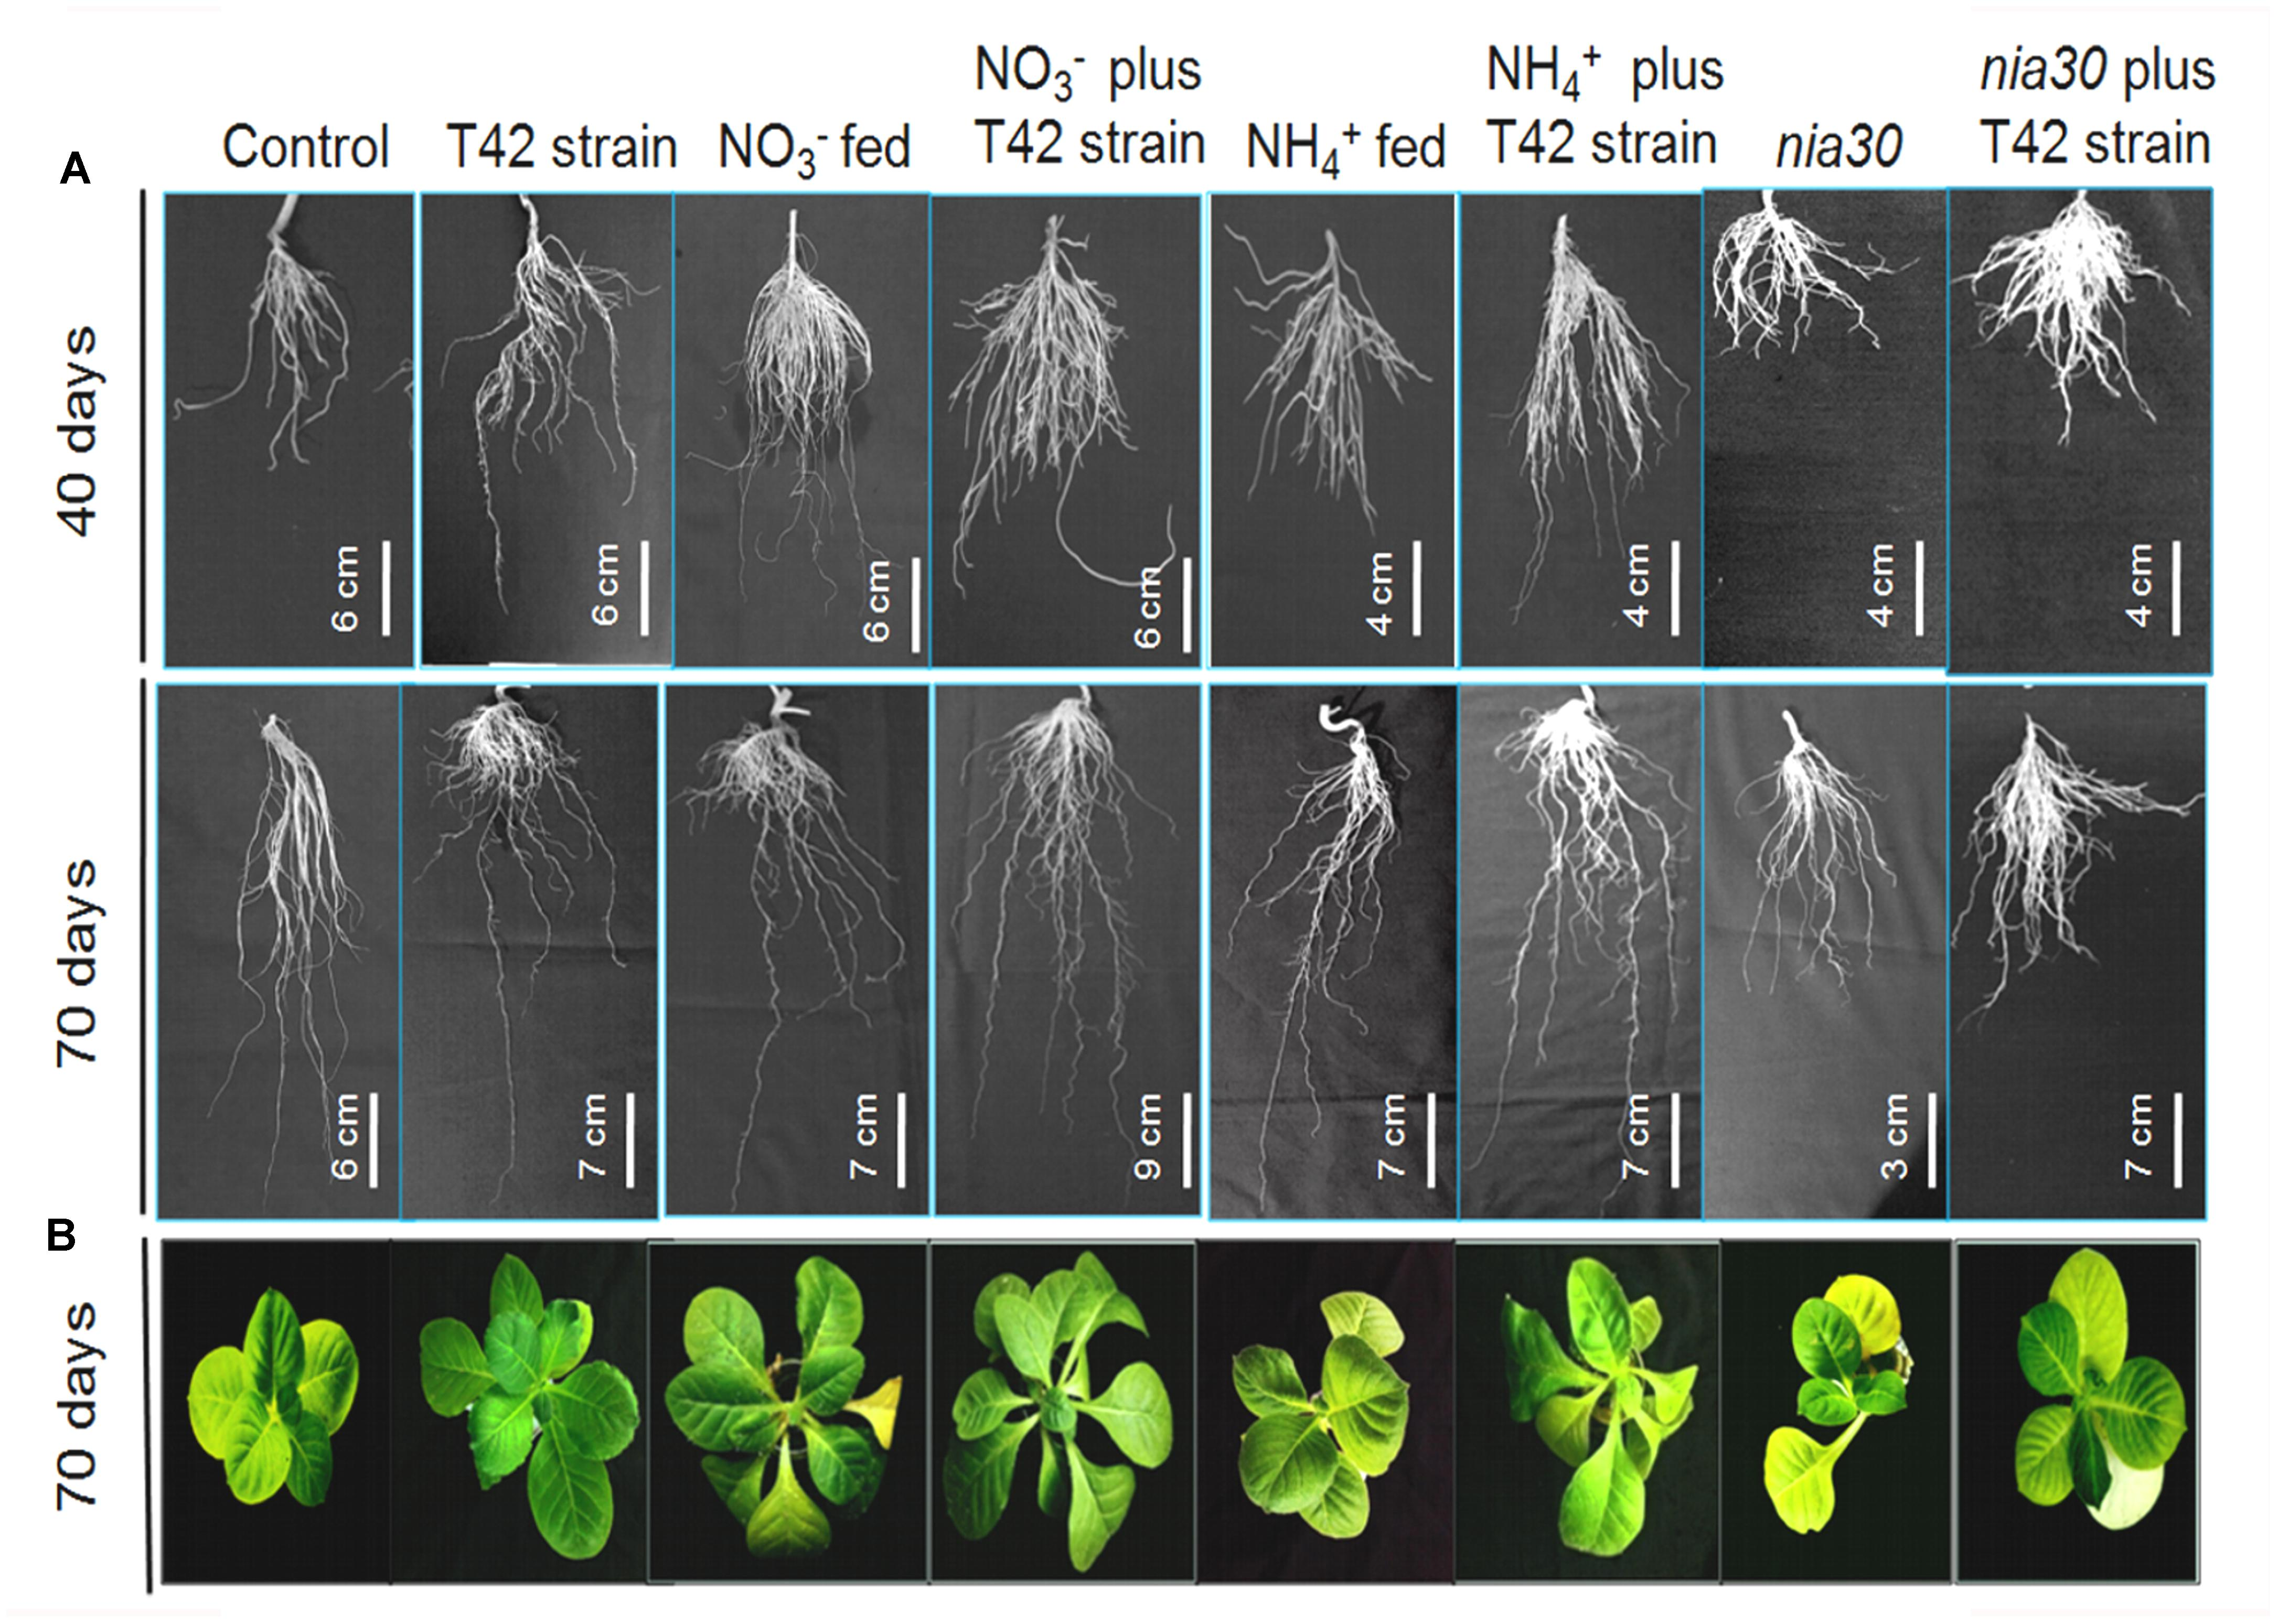
\includegraphics[trim= 10 70 10 0,clip, width=0.6\textwidth]{rootMorphology.jpg}
%     \caption{Root morphology in response to flooded soil, as in \cite{PURNOBASUKI20182012} which demonstrates the different root responses to varying nutrient and moisture content in the soil.}
%     \label{fig:roots}
% \end{figure}

Each of these roots is made up of many layers of different kinds of tissue. What is important for our model is the existence of a cell wall and membrane that nutrients must pass through to be absorbed, then using the various translocation methods these are then spread around the plant. The root tip is covered by a single shell-like covering called the root cap. The root cap allows the root to push down into the soil without any important parts of its surface being damaged in the process. Because of its protective purpose, the root cap is tougher and, for our purposes, considered largely inert and thus in our model we will not account for anything being exuded or absorbed through it. Behind the root cap there is a zone of exudation within which the plant may exude certain chemicals out into the soil. These include mainly primary metabolites such as sugars, amino acids and organic acids which may interact with the soil environment in ways which benefit the plant. For example, they may work to break down compounds which can not be readily absorbed, and can then be processed by the plant. 

% \begin{figure}[h]
%     \centering
%     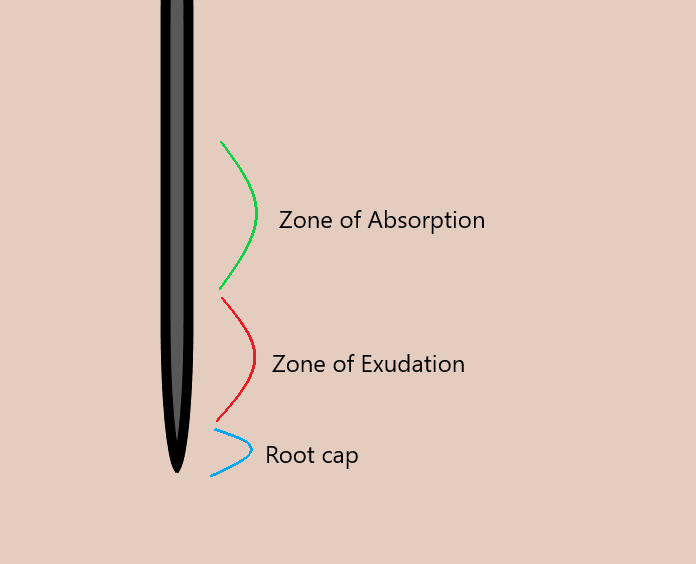
\includegraphics[width=0.25\textwidth,trim=50 20 100 20,clip]{Zonesdiagram.png}
%     \caption{Diagram showing the zones of various activity on an example plant root.}
%     \label{fig:zones}
% \end{figure}

\begin{figure}
\centering
\begin{minipage}{.5\textwidth}
    \centering
    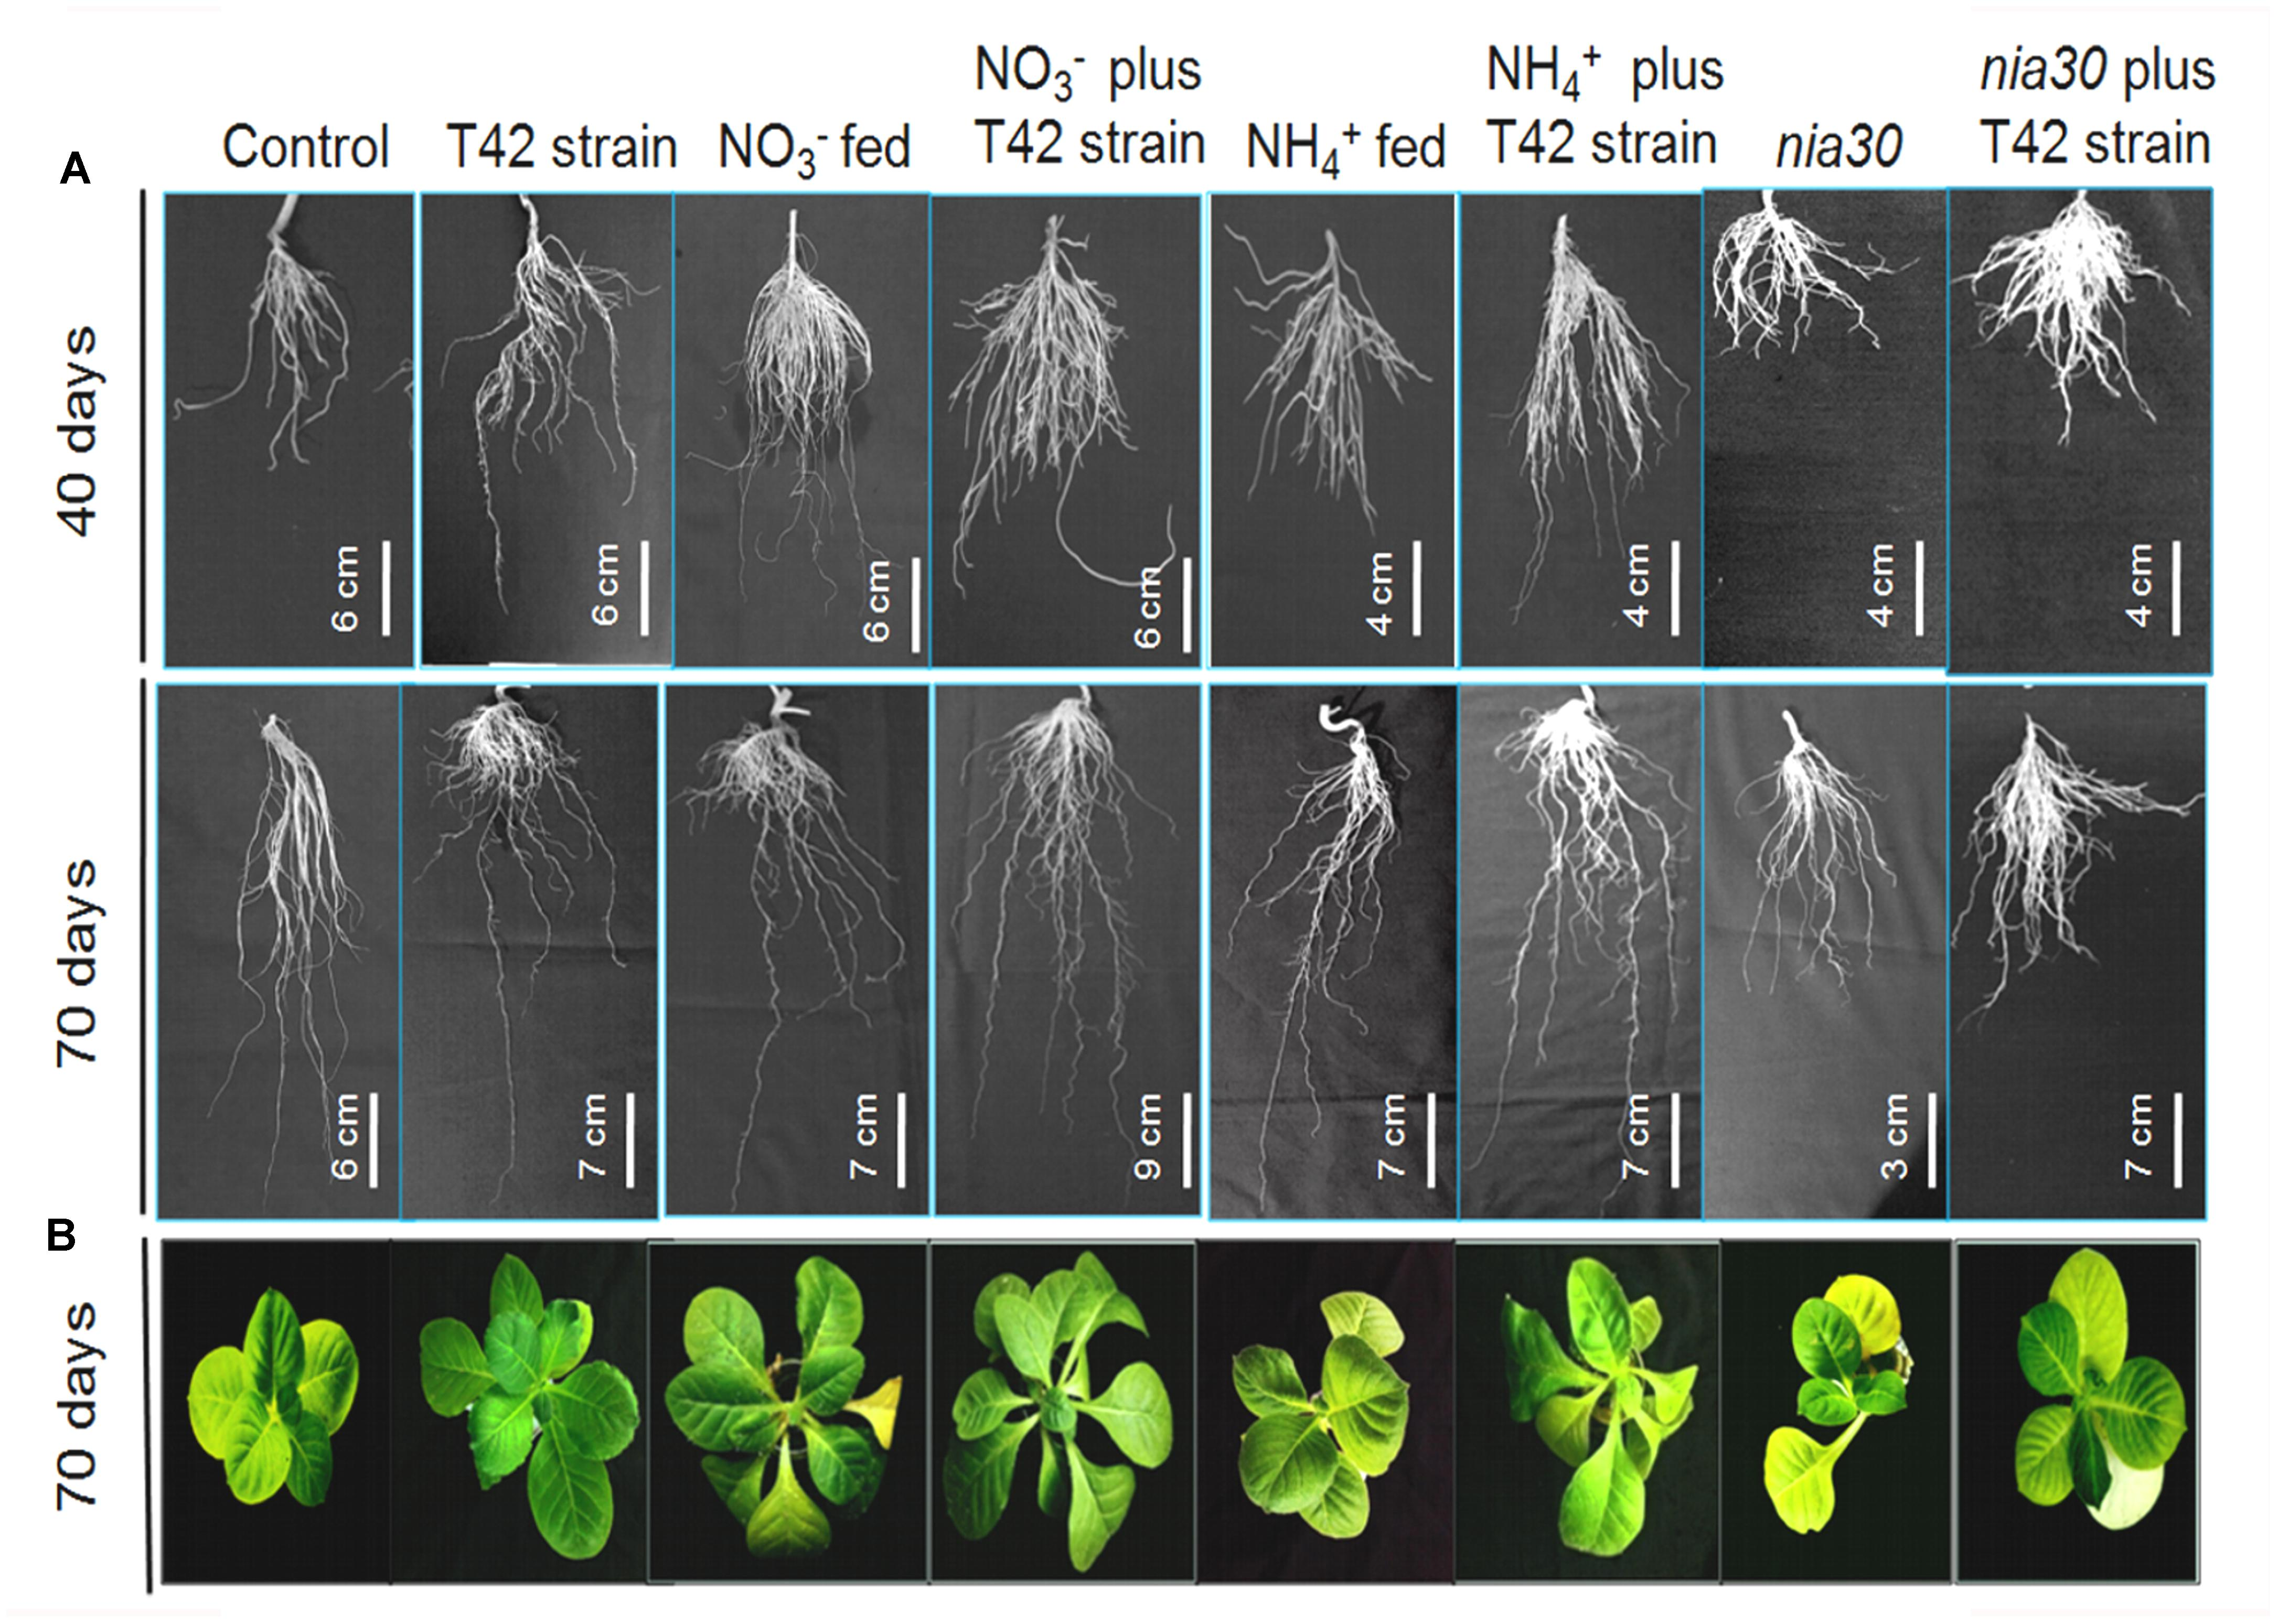
\includegraphics[width=\linewidth,trim= 10 70 10 0,clip]{rootMorphology.jpg}
    \caption{Root morphology in response to flooded soil, \\ as in \cite{PURNOBASUKI20182012} which demonstrates the different root responses\\ to varying nutrient and moisture content in the soil.}
    \label{fig:roots}
\end{minipage}%
\begin{minipage}{.5\textwidth}
  \centering
    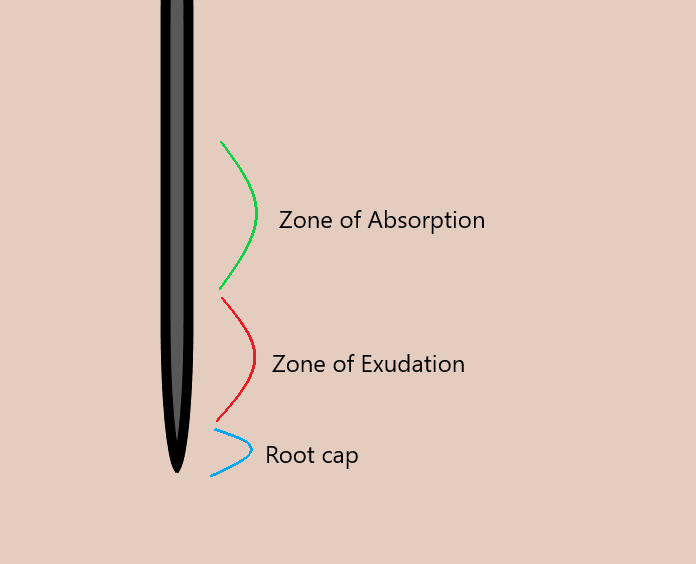
\includegraphics[width=.5\linewidth,trim=50 20 100 20,clip]{Zonesdiagram.png}
    \caption{Diagram showing the zones of various activity on an example plant root.}
    \label{fig:zones}
\end{minipage}
\end{figure}

% There is then another zone, that of absorption. 
Another zone of the root important for our model is the absorption zone. In some plants, the whole root may absorb nutrients, while in others, absorption is limited to a smaller portion of the root surface. This is similar to the zone of exudation which in some plants may be very large and in others is limited to a very small region just behind the root cap. See Fig. \ref{fig:zones} for a diagram of this and the other key zones of a sample root.

Within the absorption zone, roots absorb many different kinds of particles from the soil. While the model in \cite{Ptashnyk-2011} is focusing on zinc uptake, our primary focus in this report is the uptake of phosphorus. Both of these nutrients can be highly deficient in many soil types and interact similarly with different exudates.

\subsubsection{Interaction of exudates with soil}
% Now that we have discussed the sections of the root and how they act we can consider the ways in which they interact with our soil solution. 
% Lets consider the mechanisms at work between the root and the soil solution with interaction between our exudates and the nutrients we are considering. 
In the case of zinc  gathering, the plant exudes a phytosiderophore, deoxymugineic acid (DMA) which acts to increase the uptake of $Zn$ from soils in the form of $Zn^{2+}$ and $Zn-DMA$ at the root surface, see Fig. \ref{fig:Zinc} for an image of this in process. In the case of phosphorus, the interaction is a little more complex. First, we have the exudation of phytase enzymes which are responsible for the process of mineralising $P$, i.e. converting the unusable organic $P$ into inorganic $P$ which can then be processed by the plant. Then studies have shown that in soil with limited $P$ availability, exudation of citrate by plant roots has improved $P$ solubalisation in soils, allowing the now inorganic $P$ to move from solid soil into our solution and thus move through the soil by the processes of diffusion and convection. Most importantly, research has shown that working in tandem, citrate and phytase have a much larger effect on $P$ absorption than we can currently explain, thus we have chosen to model the exudation of both rather than taking models of each single exudate by itself \cite{giles_george}.

\begin{figure}[h]
\centering
\begin{subfigure}[t]{0.4\textwidth}
    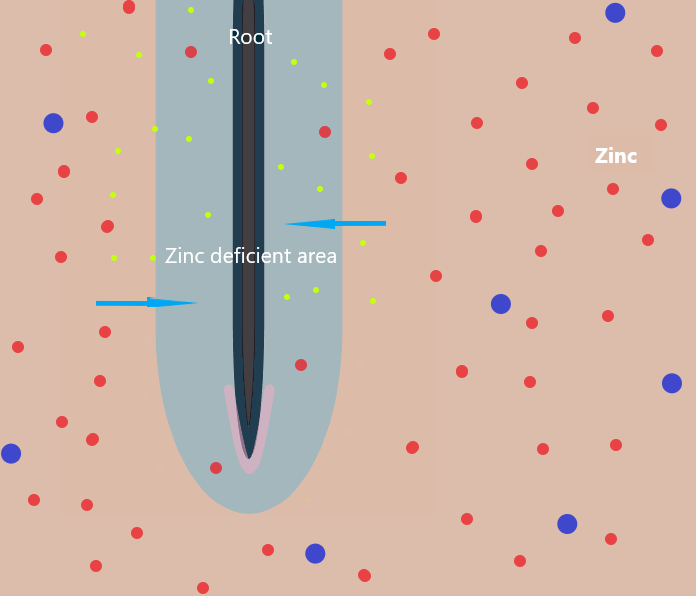
\includegraphics[width=\textwidth]{RootZincDiagram.png}
    \caption{
    % Diagram showing the exudation of DMA, shown in green, by the plant roof to improve Zinc, shown in red, solubility and cause it to move into the deficient area. This also shows the presence of microbes in the soil, shown in purple, which will consume the DMA.
    }
    \label{fig:Zinc}
\end{subfigure}
% \hfill
\qquad
\begin{subfigure}[t]{0.4\textwidth}
    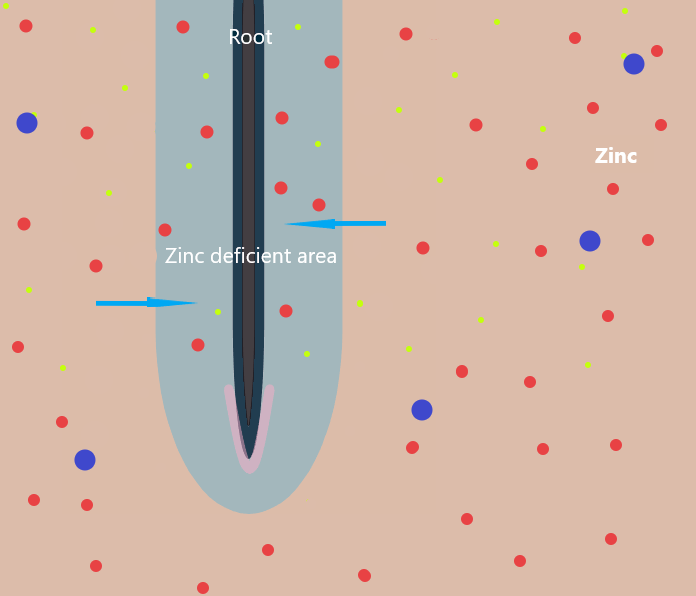
\includegraphics[width=\textwidth]{RootZincDiagram2.png}
    \caption{
    % Diagram showing the movement of Zinc, in red, in response to DMA exudation, in green, and the consumption of DMA by microbes, in purple.
    }
    \label{fig:my_label}
\end{subfigure}
\caption{Diagrams showing the dynamics of the exudate DMA (green) with $Zn$ (red) in the soil; (a) DMA improves $Zn$ solubility and causes it to move into the deficient area, presence of microbes (purple); (b) movement of $Zn$ in response to DMA exudation and the consumption of DMA by microbes.}
\end{figure}


\subsection{Base model formulation}
% In our initial model we expand on 
To start with, we introduce work done by \cite{Ptashnyk-2011} which considers the way rice plants access $Zn$ in $Zn$-deficient soils. The paper models the mechanism of DMA exudation which allows rice roots to access $Zn$ and form $Zn$-DMA which is solubilised as explained in the previous sections. Let $X$ be the amount of the micronutrient metal $Zn$ and $Y$ the amount of exuded phytosiderophore DMA. First the soil is modelled as a solution of water and solid soil particles, with the equations allowing for adsorption and desorption to occur on soil surfaces as well as diffusion only within the solution and not the sorbed state. We can split $X$ and $Y$ into the amount of each in he different states, let $X_L$, $Y_L$ be the concentrations of $Zn$ and DMA in solution and $X_S$, $Y_S$ are the concentrations in soil solids. Thus we obtain the conservation equations for $X$ and $Y$ in one unit volume of soil,
% \begin{align}
%     \partial_t(\theta X_L+X_S)&=\nabla (D_X\nabla X_L-\nu X_L)-g_X,\\
%     \partial_t(\theta Y_L+Y_S)&=\nabla (D_Y\nabla Y_L-\nu Y_L)-g_Y,\\
% \end{align}
\begin{equation}
    \begin{aligned}
        \partial_t(\theta X_L+X_S)&=\nabla (D_X\nabla X_L-\nu X_L)-g_X,\\
        \partial_t(\theta Y_L+Y_S)&=\nabla (D_Y\nabla Y_L-\nu Y_L)-g_Y,\\
    \end{aligned}
    \label{eq:1}
\end{equation}
with coefficients as summarised in Table \ref{t:First-model-params}. We can then derive equilibrium conditions between the soil particles and solution. At equilibrium, there will be no change in the amount of DMA or $Zn$ in solution, thus we know
\begin{equation}
    \begin{aligned}
        \partial_t X_s&=\beta_1X_L-\beta_2X_S-\beta_3X_SY_L=0,\\
        \partial_tY_S&=\gamma_1Y_L-\gamma_2Y_S-\gamma_3Y_SX_L=0,\\
    \end{aligned}
    \label{eq:2}
\end{equation}
with $\beta_1,\beta_2,\beta_3,\gamma_1,\gamma_2,\gamma_3$ being the reaction rate coefficients.


If we differentiate equation \eqref{eq:1} and substitute this into the system \eqref{eq:2}, we obtain our final equations
\begin{align}
    \left( \theta + \frac{b_X}{1 + \kappa_X b_X Y_L} \right) \partial_t X_L - \frac{\kappa_X b_X^2 X_L}{(1+\kappa_X b_X Y_L)^2} \partial_t Y_L &=
    \nabla \cdot ( D_X \nabla X_L - \nu X_L  ) - g_X,
    \label{eq:sys-Zn-X-Omega}
    \\
    \left( \theta + \frac{b_Y}{1 + \kappa_Y b_Y X_L} \right) \partial_t Y_L - \frac{\kappa_Y b_Y^2 Y_L}{(1+\kappa_Y b_Y X_L)^2} \partial_t X_L &=
    \nabla \cdot ( D_Y \nabla Y_L - \nu Y_L  ) - g_Y.
\end{align}
Having derived the system of equations, we must now determine the conditions on the boundary of our region of consideration.
The concentrations of $X$ and $Y$ depend upon two spacial variables in $\R^2$, $(r,z)$ which measure radial distance from the center of the  root, and length from the soil surface respectively as shown in figure \ref{fig:geom}. 
In this model we have the presence of a single plant root on one vertical edge (on the left-hand side of the domain) and a zero-flux boundary on the other:
\begin{align}
    D_X \partial_r X_L - \nu X_L &= \alpha X_L & \text{at } r = a, z \in [L - \delta L_X, L], \\
    D_Y \partial_r Y_L - \nu Y_L &= -F_Y(t) &\text{at } r = a, z \in [L - \delta L_Y, L].
\end{align}
with
\begin{equation}
     D_X \partial_r X_L - \nu X_L = 0
    \qquad\text{and}\qquad
    D_Y \partial_r Y_L - \nu Y_L = 0 \qquad\text{at}\, r = x.
\end{equation}
These boundary conditions represent the exudation of DMA from the root surface, as well as the absorption of $Zn$ from the soil surrounding the root. In particular we have $F_Y(t)$, the rate of exudation of DMA, initially we keep this as a function of time however the conclusions of the aforementioned paper allow us to eventually keep it as a constant over 24 hours.
\begin{figure}
    \centering
    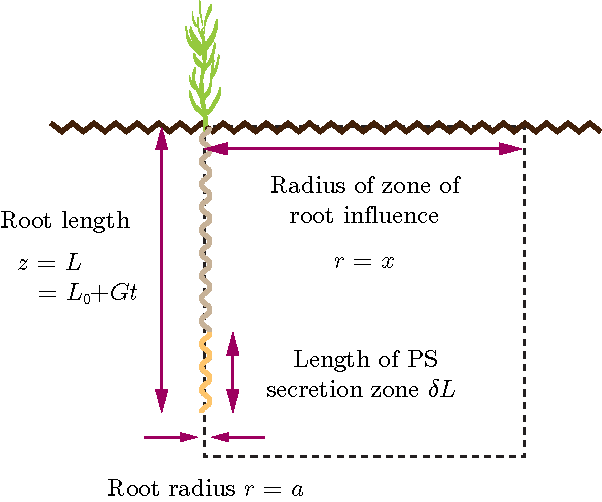
\includegraphics[scale=0.7]{Figures/First-plot.pdf}
    \caption{Sketch of the domain for system with one plant as in \cite{Ptashnyk-2011}. The root portrayed is curly for illustration.}
    \label{fig:geom}
\end{figure}
\newpage
%%%%%%%%%%%%%%%%%%%%%%%%%%%%%%%%%%%%%%%%%%%%%%%%%%%

\section{Base model}

In the following section we will focus on the following nonlinear system of PDEs:
\begin{subequations}
\label{eq:system-Zinc}
\begin{align}
    \left( \theta + \frac{b_X}{1 + \kappa_X b_X Y_L} \right) \partial_t X_L - \frac{\kappa_X b_X^2 X_L}{(1+\kappa_X b_X Y_L)^2} \partial_t Y_L &=
    \nabla \cdot ( D_X \nabla X_L - \nu X_L  ) - g_X
    \label{eq:sys-Zn-X-Omega}
    \\
    \left( \theta + \frac{b_Y}{1 + \kappa_Y b_Y X_L} \right) \partial_t Y_L - \frac{\kappa_Y b_Y^2 Y_L}{(1+\kappa_Y b_Y X_L)^2} \partial_t X_L &=
    \nabla \cdot ( D_Y \nabla Y_L - \nu Y_L  ) - g_Y;
\end{align}
where $X(r,z)$ and $Y(r,z)$ are subject to the boundary conditions:
\begin{align}
    D_X \partial_r X_L - \nu X_L &= \alpha X_L & \text{at } r = a, z \in [L - \delta L_X, L],
    \label{eq:sys-Zn-X-Gamma-a}
    \\
    D_Y \partial_r Y_L - \nu Y_L &= -F_Y(t) &\text{at } r = a, z \in [L - \delta L_Y, L],
\end{align}
where $L = L_0 + G t$. For the rest of the boundary, we have zero-flux conditions; i.e., in the case \( r = x\), this is just
\begin{align}
    D_X \partial_r X_L - \nu X_L = 0
    \label{eq:sys-Zn-X-Gamma-x}
    \qquad\text{and}\qquad
    D_Y \partial_r Y_L - \nu Y_L = 0.
\end{align}
Moreover, $r \in [a,x]$, with $x = (\pi L_V)^{1/2}$, and $z \in [0, L_{t_{\mathrm{max}} }]$. The meaning of these parameters is presented in Table \ref{t:First-model-params}.
\end{subequations}


%%%%%%%%%%%%%%%%%
%%%%%%%%%%%%%%%%%
\subsection{Variational formulation}


The existence of a solution to model \eqref{eq:system-Zinc} is presented in Section \ref{sec:Existence}.
To find the variational formulation of system \eqref{eq:system-Zinc}, we will use a sufficiently smooth test function and then use a density argument for a more general function space. Let's begin supposing that there is a $\mathcal{C}^2 (\bar \Omega)$ solution pair $(X_L,Y_L)$ and multiply the first equation by a $v \in \mathcal{C}^1 (\bar\Omega)$ function and introduce $A_X(Y_L) = \theta + \frac{b_X}{1 + \kappa_X b_X Y_L}$ and $B_X(X_L,Y_L) = \frac{\kappa_X b_X^2 X_L}{(1+\kappa_X b_X Y_L)^2}$. We then get
\begin{align}
    A_X(Y_L) \partial_t X_L v - B_X(X_L,Y_L) \partial_t Y_L v = \nabla \cdot (D_X \nabla X_L - \nu X_L) v - g_X v.
\end{align}
Integrating this with respect to the pair \(x = (r,z)\), and using the Divergence Theorem, we have
\begin{align}
    \int\limits_\Omega
    A_X(Y_L) \partial_t X_L v &- B_X(X_L,Y_L) \partial_t Y_L v \dif \mu = 
    \int\limits_\Omega
    \nabla \cdot (D_X \nabla X_L - \nu X_L) v  \dif \mu
    -\int\limits_\Omega g_X v \dif \mu
    \\
    &=
    \int\limits_\Gamma
    (D_X \nabla X_L - \nu X_L) \cdot \vec{n} v
    \dif \sigma
    -\int\limits_\Omega
    (D_X \nabla X_L - \nu X_L) \cdot \nabla v  \dif \mu
    -\int\limits_\Omega g_X v \dif \mu;
\end{align}
where $\Gamma$ is the boundary of $\Omega$, $\vec{n}$ its normal vector and $\sigma$ the surface measure on $\Gamma$. 

Notice that we only need to analyse three segments of $\Gamma$: $\Gamma_{a_X} = \{a\}\times [L-\delta L_X,L]$, $\Gamma_{a_Y} = \{a\} \times [L - \delta L_Y, L]$, and $ \Gamma_0 = \Gamma \setminus (\Gamma_{a_X} \cup \Gamma_{a_Y})$. At $r = a$, we have that $ \vec{n} = (-1,0)$, thus
\begin{align}
    \int\limits_{\Gamma_{a_X}}
    (D_X \nabla X_L - \nu X_L) \cdot \vec{n} v    \dif \sigma
    =
    -
    \int\limits_{\Gamma_{a_X}}
    (D_X \partial_r X_L - \nu X_L) v    \dif \sigma
    =
    -\int\limits_{\Gamma_{a_X}}
    \alpha X_L v    \dif \sigma.
\end{align}
Similarly, in the equation for \(Y_L\) we have
\begin{align}
    \int\limits_{\Gamma_{a_Y}}
    (D_Y \nabla Y_L - \nu Y_L) \cdot \vec{n} v    \dif \sigma
    =
    \int\limits_{\Gamma_{a_Y}}
    F_Y(t) v    \dif \sigma.
\end{align}
For the other segments of the border, the surface area is zero. To see this, consider $r = x$, where we have that $ \vec{n} = (1,0)$, thus
\begin{align}
    \int\limits_{\Gamma_0 \cap \{r=x\}}
    (D_X \nabla X_L - \nu X_L) \cdot \vec{n} v    \dif \sigma
    =
    \int\limits_{\Gamma_0 \cap \{r=x\}}
    (D_X \partial_r X_L - \nu X_L) v    \dif \sigma
    =
    0.
\end{align}

As a result, we have that the following equation must be satisfied for every $v \in \mathcal{C}^1 (\bar\Omega)$:
\begin{align}
    \int\limits_\Omega
    A_X(Y_L) \partial_t X_L v - B_X(X_L,Y_L) \partial_t Y_L v \dif \mu
    &=
    -\int\limits_{\Gamma_{a_X}}    \alpha X_L v    \dif \sigma
    -\int\limits_\Omega        (D_X \nabla X_L - \nu X_L) \cdot \nabla v  \dif \mu
    -\int\limits_\Omega        g_X v \dif \mu.
\end{align}
Notice that by density, the weak form of the previous equation is the same over $H^1(\Omega)$.
Similarly, the variational form for the governing equation of $Y_L$ is
\begin{align}
    \int\limits_\Omega
    A_Y(X_L) \partial_t Y_L v - B_Y(Y_L,X_L) \partial_t X_L v \dif \mu
    &=
    \int\limits_{\Gamma_{a_Y}}     F_Y(t) v    \dif \sigma
    -\int\limits_\Omega        (D_Y \nabla Y_L - \nu Y_L) \cdot \nabla v  \dif \mu
    -\int\limits_\Omega        g_Y v \dif \mu 
\end{align}
for all \(v \in H(\Omega)\).



%%%%%%%%%%%%%%%%%
%%%%%%%%%%%%%%%%%
\subsection{Time discretisation}

To approximate the time derivative we will use a simple backward difference. First, we will discretise the time domain; then, let the superscript $n$ denote a quantity at time $t_n$, where $n$ is an integer counting time levels; e.g. $X_L^n$ is $X_L$ evaluated at time level $n$. This yields
\begin{equation}
    \left(\frac{\partial X_L}{\partial t}\right)^{n+1} \approx \frac{X_L^{n+1} - X_L^n}{\Delta t}.
\end{equation}
Inserting this in the variational formulation, we get the approximation
\begin{equation}
\begin{aligned}
    \int\limits_\Omega
    \big(
    A_X(Y_L^{n+1}) &(X_L^{n+1} - X_L^n) - B_X(X_L^{n+1},Y_L^{n+1}) (Y_L^{n+1} - Y_L^n)  
    \big) v \dif \mu
    \\
    &+
    \Delta t \int\limits_\Omega        (D_X \nabla X_L^{n+1} - \nu X_L^{n+1}) \cdot \nabla v  \dif \mu
    +
    \Delta t \int\limits_{\Gamma_{a_X^{n+1}}}    \alpha X_L^{n+1} v    \dif \sigma
    =
    -\Delta t \int\limits_\Omega        g_X v \dif \mu.
\end{aligned}
\end{equation}
In the case of $Y_L$, we proceed with the same time scale and get
\begin{equation}
\begin{aligned}
    \int\limits_\Omega
    \big(
        A_Y(X_L^{n+1}) & (Y_L^{n+1} - Y_L^n)  - B_Y(Y_L,X_L) (X_L^{n+1} - X_L^n)
    \big) v \dif \mu
    \\
    &
    + \Delta t\int\limits_\Omega        (D_Y \nabla Y_L^{n+1} - \nu Y_L^{n+1}) \cdot \nabla v  \dif \mu
    =
    \Delta t\int\limits_{\Gamma_{a_Y^{n+1}}}     F_Y(t_{n+1}) v    \dif \sigma
    -\Delta t\int\limits_\Omega        g_Y v \dif \mu.
\end{aligned}
\end{equation}

Notice that we further need to approximate the system at time \(t=0\). At this level, we will set \( (X_L^0,Y_L^0)\). Moreover, this discretisation is also useful for the non-dimensionalised formulation.



\begin{table}[!htb]
\begin{center}
% \caption{Table of parameters and their meanings for base model.}
\fontsize{9.5}{7}\selectfont
\setlength{\tabcolsep}{5.pt}
\def\arraystretch{2.0}
\begin{tabular}{cl}
\toprule
    \bf Symbol & \multicolumn{1}{c}{\bf Meaning}
    %
    \\ \midrule
    $D_X$ & Diffusion of the metal (e.g. Zn) in the soil, $D_X = D_{L,X} \theta f$  \\  
	$D_{Y}$ &  Diffusion of the PS $Y$ in the soil, $D_{Y} = D_{L,Y} \theta f$  \\ 
	$\nu$ & Water flux\\
	$g_X$ & Function for the metal (Zn) immobilisation \\
	$g_{Y}$ & Function for decomposition of $Y_1$ \\
	$b_X$ & Metal buffer power \\
	$b_{Y}$ & PS $Y$ buffer power \\
	$\kappa_{X}$ & $X$ - $Y$ interaction coefficient \\
	$\kappa_{Y}$ & $Y$ - $X$ interaction coefficient\\
	$\alpha $ & Metal-absorbing power of root \\
	$F_{Y} $ & Rate of PS $Y$ exudation over 24h \\
	$L$ & Length of root at certain time, increases at rate $G$ \\
	$\delta L_{X}$ & Length of metal uptake zone \\
	$\delta L_{Y}$ & Length of PS $Y$ uptake zone  \\	
	$a$ & Root radius of plant \\
\bottomrule
\end{tabular}
\caption{Table of parameters and their meanings for base model.
\label{t:First-model-params}}
\end{center}
\end{table}







%%%%%%%%%%%%%%%%%%%%%%%%%%%%%%%%%%%%%%%%%

\subsection{Numerical solution}
To numerically solve the system in FEniCS, we use the variational formulation discretised in time defined in the previous subsections. Since the problem is nonlinear, we can linearise it by using the solution computed in the previous time step. First, we solve the equation for $Y$, (insert eq), followed by the equation for $X$ \textcolor{red}{FINISH the computational formulation}.

In FEniCS, we define the boundaries as the edges of the rectangular domain. However, our boundary conditions are not valid on the whole edge but only on a part of it (along the whole root or its part), 

therefore we define two indicator functions. The first indicator function should attain 1 when on the part of the domain where the uptake of a nutrient happens. This is by assumption along the whole root ($\delta L_X =0$), which has length $L_0 + Gt$, where $L_0$ is the length of the root at the beginning of the simulation, $G$ is the growth rate in dm/day, and $t$ is time in days. Thus, the indicator function should act on the interval $$0 \geq z \geq -(L_0 + Gt),$$ as the root is growing downwards - to the negative part of the z-dimension. We would prefer for the indicator function to not be a step function as its discontinuity is likely to cause numerical issues. We therefore opt for $\arctan(z)$, which we modify to 
\begin{equation}
    I_1 (z) = \frac{1}{\pi} \arctan(c (z+(L_0 + Gt))) + \frac{1}{2},
\end{equation}
where $c$ manipulates the steepness of the function. The multiplication by $\frac{1}{\pi}$ and addition of $\frac{1}{2}$ sets the range of the function from $0$ to $1$ with $\lim_{z \to \infty} I_1(z) = 1$, $\lim_{z \to -\infty} I_1(z) = 0$.

The second indicator function will be used for the exudation boundary condition at $$-(L_0 + Gt - \delta L_Y) \geq z \geq -(L_0 + Gt).$$ Similarly to the previous function, we achieve values close to $1$ by a combination of $\arctan(z)$ functions,
\begin{equation}
    I_2 (z) = \frac{1}{\pi} [ \arctan(c (z+(L_0 + Gt + d))) - \arctan(c (z+(L_0 + Gt -\delta L_Y - d))) ],
\end{equation}
with $d$ controlling the point behind root tip where exudation starts happening (in the experiments we used both $d = 2$ cm and $\delta L_Y = 2$ cm, i.e. the plants is exuding at a 2 cm long region located 2 cm behind the root tip).

\textcolor{red}{INSERT SOME RESULTS TO SHOW THE RICE MODEL?}

\textcolor{red}{SHOW EXTENSION OF THE BCS TO THE 2-ROOT SYSTEM}

\begin{figure}[h]
    \centering
    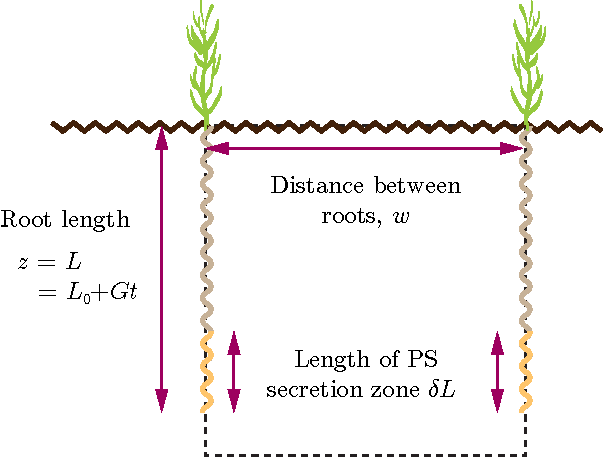
\includegraphics[scale=0.7]{Figures/Second-plot.pdf}
    \caption{Sketch of the domain for system with two plants and one exudate.}
    \label{fig:2roots-a}
\end{figure}

\subsection{Some results}


\newpage
%%%%%%%%%%%%%%%%%%%%%%%%%%%%%%%%%%%%%%%%%
%%%%%%%%%%%%%%%%%%%%%%%%%%%%%%%%%%%%%%%%%
\subsection{Scaling}
\label{2-Base-Scaling}

A drawback of model \eqref{eq:system-Zinc} is that numerical schemes for solving it might perform poorly if the parameters associated to the model are too small. This is actually the case, in the setting of Zinc uptake. As a result, we will scale the variables of the model appropriately. For this end, we introduce the following relations
\[
    r = \varepsilon_r \hat{r} + a,
    \qquad
    z = \varepsilon_z \hat{z},
    \qquad
    t = \varepsilon_t \hat{t},
    \qquad
    X_L = \varepsilon_x \hat{x},
    \qquad
    Y_L = \varepsilon_y \hat{y};
\]
where \( \varepsilon_r, \varepsilon_z, \varepsilon_t, \varepsilon_x, \varepsilon_y\) are scaling constants to be determined, and \(\hat{r}, \hat z, \hat t, \hat x, \hat y\) are non-dimensional variables.
Clearly, we have the relation \(X_L(r,z) = \varepsilon_x \hat{x} (\varepsilon_r \hat r + a, \varepsilon_z \hat z) = \varepsilon_x \hat{x} \big( \varepsilon_r^{-1} (r-a) , \varepsilon_z^{-1} z\big) \) and similarly \(Y_L (r,z) = \varepsilon_y \hat{y} \big( \varepsilon_r^{-1} (r-a), \varepsilon_z^{-1} z \big)\). Using this, we see that the gradient operator is also scaled as
\[
    \nabla X_L =
    \begin{pmatrix}
        \nicefrac{1}{\varepsilon_r} & 0 \\
        0 & \nicefrac{1}{\varepsilon_z}
    \end{pmatrix}
    \hat{\nabla} \varepsilon_x \hat{x},
    \qquad \text{with} \qquad
    \hat{\nabla} = 
    \begin{pmatrix}
        \pd{ }{\hat r}
        &
        \pd{ }{\hat z}
    \end{pmatrix}^\top .
\]
The scaled equations are easy to determine. For instance,  \eqref{eq:sys-Zn-X-Omega} is measured in \si{M.s^{-1}}, which are the units that \(\varepsilon_x\) and \(\varepsilon_t^{-1}\) correspond to. For the left-hand side we have that
\begin{align}
    \left( \theta + \frac{b_X}{1 + \kappa_X b_X Y_L} \right) \partial_t X_L &= \frac{\varepsilon_x}{\varepsilon_t} \left( \theta + \frac{b_X}{1 + \varepsilon_y \kappa_X b_X \hat{y}} \right)  \pd{\hat{x}}{\hat{t}}
    \\
    - \frac{\kappa_X b_X^2 X_L}{(1+\kappa_X b_X Y_L)^2} \partial_t Y_L &=
    -\frac{\varepsilon_x}{\varepsilon_t} \frac{\varepsilon_y \kappa_X b_X^2 \hat{x}}{(1+ \varepsilon_y\kappa_X b_X \hat{y})^2} \pd{\hat y}{\hat t}
\end{align}
The right-hand side requires some care. As \(\nu\) is measured in \si{dm.s^{-1}}, we introduce the non-dimensional quantities \( \hat{\nu}_r\) and \( \hat{\nu}_z\) such that \( \nu = \nicefrac{\varepsilon_r}{\varepsilon_t} \hat{\nu}_r \) and \( \nu = \nicefrac{\varepsilon_z}{\varepsilon_t} \hat{\nu}_z \). Likewise, \(D_X\) is measured in \si{dm^2.s^{-1}}, and we can proceed as before introducing two non-dimensional constants such that \(D_{X} = \nicefrac{\varepsilon_r^2}{\varepsilon_t} \hat{D}_{X,r}\) and \(D_{X} = \nicefrac{\varepsilon_z^2}{\varepsilon_t} \hat{D}_{X,z}\). This way, we have that
\begin{align}
    \nabla \cdot ( D_X \nabla X_L - \nu X_L  )
    &=
    \begin{pmatrix}
        \nicefrac{1}{\varepsilon_r} & 0 \\
        0 & \nicefrac{1}{\varepsilon_z}
    \end{pmatrix}
    \hat{\nabla}
    \cdot
    \left( 
        D_X
        \varepsilon_x
        \begin{pmatrix}
        \nicefrac{1}{\varepsilon_r} & 0 \\
        0 & \nicefrac{1}{\varepsilon_z}
    \end{pmatrix}
    \hat{\nabla} \hat{x} - \nu \varepsilon_x \hat{x}
    \right)
    \notag
    \\
    &= \varepsilon_x
    \begin{pmatrix}
        \nicefrac{1}{\varepsilon_r} & 0 \\
        0 & \nicefrac{1}{\varepsilon_z}
    \end{pmatrix}
    \hat{\nabla}
    \cdot
    \left( 
        \begin{pmatrix}
         \nicefrac{\varepsilon_r}{\varepsilon_t} \hat{D}_{X,r} & 0 
         \\
        0 &  \nicefrac{\varepsilon_z}{\varepsilon_t} \hat{D}_{X,z}
    \end{pmatrix}
    \hat{\nabla} \hat{x} - \hat{x}
    \begin{pmatrix}
         \nicefrac{\varepsilon_r}{\varepsilon_t} \hat{\nu}_{r} 
         \\
        \nicefrac{\varepsilon_z}{\varepsilon_t} \hat{\nu}_{z}
    \end{pmatrix}
    \right)
    \notag
    \\
    &= \frac{\varepsilon_x}{\varepsilon_t}
    \hat{\nabla}
    \cdot
    \left( 
        \begin{pmatrix}
         \hat{D}_{X,r} & 0 
         \\
        0 &  \hat{D}_{X,z}
    \end{pmatrix}
    \hat{\nabla} \hat{x} - \hat{x}
    \begin{pmatrix}
         \hat{\nu}_{r} 
         \\
        \hat{\nu}_{z}
    \end{pmatrix}
    \right)
    \label{eq:divergence-non-dimen-x}
\end{align}
For \(g_X\) we can proceed as we did for \eqref{eq:divergence-non-dimen-x} by noticing that its measured in \si{M.s^{-1}} and introduce the non-dimensional quantity \( \frac{\varepsilon_x}{\varepsilon_t}\hat{g}_{x} = g_X\).

Similarly, in the case of the boundary conditions, we have that \eqref{eq:sys-Zn-X-Gamma-a} is equivalent to
\[
    D_X \partial_r X_L - \nu X_L = 
    \frac{\varepsilon_r^2}{\varepsilon_t} \hat{D}_{X,r} \frac{\varepsilon_x}{\varepsilon_r} \pd{\hat{x}}{\hat{r}} - \frac{\varepsilon_r}{\varepsilon_t} \hat{\nu}_r \varepsilon_x \hat{x} = \frac{\varepsilon_r \varepsilon_x}{\varepsilon_t} \hat{\alpha} \hat{x}
    \qquad \text{at } r = a = a + \varepsilon_r \hat{r}, \varepsilon_z \hat{z} \in [L - \delta L_X, L],
\]
or equivalently
\begin{equation}
    \label{eq:sys-Zn-nond-a}
    \hat{D}_{X,r} \pd{\hat{x}}{\hat{r}} - \hat{\nu}_r \hat{x} = \hat{\alpha} \hat{x}
    \qquad \text{at } \hat{r} = 0, \hat{z} \in [\hat{L} - \delta \hat{L}_x, \hat{L}];
\end{equation}
where we require \( \alpha = \nicefrac{\varepsilon_r}{\varepsilon_t} \hat{\alpha}\), \( \hat{L} = \varepsilon_z^{-1} L\), and \( \delta\hat{L}_x = \varepsilon_z^{-1} \delta L_X\). Finally, condition \eqref{eq:sys-Zn-X-Gamma-x} is just
\begin{equation}
    \label{eq:sys-Zn-nond-x}
    \hat{D}_{X,r} \pd{\hat{x}}{\hat{r}} - \hat{\nu}_r \hat{x} = 0
    \qquad \text{at } \hat{r} = \frac{x-a}{\varepsilon_r}.
\end{equation}

Conditions \eqref{eq:sys-Zn-nond-a} and \eqref{eq:sys-Zn-nond-x} give us a hint of how we need to select \(\varepsilon_r\) and \(\varepsilon_z\). If we select \( \varepsilon_r = x-a\), then \( \hat{r} \) will be in the range \( [0,1]\). Similarly, if we pick \( \varepsilon_z = L_{t_{\max}}\), again \(\hat z \) will be in the range \( [0,1]\) (or \([0,-1]\) in the case \(L\leq 0\), and \(\delta L \leq 0\)). This last selection implies that the maximum absolute value of \( \hat{L}\) should be \(1\) where we have
\[
    \hat{L} = \hat{L}(\hat t) = \frac{1}{\varepsilon_z} ( L_0 + G \varepsilon_t \hat t )
    = \hat{L}_0 + \hat{G} \hat t,
    \qquad 
    \hat{L}_0 = \varepsilon^{-1}_z L_0,
    \qquad
    \hat{G} = \varepsilon_t \varepsilon_z^{-1} G;
\]
and we can further select \( \varepsilon_t = t_{\max}\) to finally have \( \hat t\) in the range \( [0,1]\). As a result, we have selected scaling parameters such that the system of partial differential equations  \eqref{eq:system-Zinc} is defined in either \( [0,1]^3\) or \([0,1]\times [0,-1] \times [0,1]\).


%%%%%%%%%%%%%%%%%%%%%%%%%%
%%%%%%%%%%%%%%%%%%%%%%%%%%
\subsubsection{Scaled variational formulation}

The weak form of the scaled system can be recomputed from the variational formulation presented for system \eqref{eq:system-Zinc} or again using the divergence theorem. %The resulting weak-system is as follows:
Let us introduce the scaled constants 
\(\hat{\kappa}_X = \varepsilon_y \kappa_X\), \(\hat{\kappa}_Y = \varepsilon_x \kappa_Y\), \(\hat{F}_y = \frac{\varepsilon_t}{\varepsilon_r \varepsilon_y} F_y \),
the constant scaled vector 
\(
    \hat{\nu} = 
    (\begin{smallmatrix}
        \hat{\nu}_r
        &
        \hat{\nu}_z
    \end{smallmatrix})^\top
    =
    \nu \varepsilon_t
    (\begin{smallmatrix}
        {\varepsilon_r}^{-1}
        &
        {\varepsilon_z}^{-1}
    \end{smallmatrix})^\top,
\) 
and the constant matrices
\[
    \hat{D}_x = 
    \begin{pmatrix}
         \hat{D}_{X,r} & 0 
         \\
        0 &  \hat{D}_{X,z}
    \end{pmatrix}
    =
    D_X \varepsilon_t
    \begin{pmatrix}
         \varepsilon_r^{-2} & 0 
         \\
        0 &  \varepsilon_z^{-2}
    \end{pmatrix}
    ,\qquad
    \hat{D}_y = 
    \begin{pmatrix}
         \hat{D}_{Y,r} & 0 
         \\
        0 &  \hat{D}_{Y,z}
    \end{pmatrix}
    =
    D_Y \varepsilon_t
    \begin{pmatrix}
         \varepsilon_r^{-2} & 0 
         \\
        0 &  \varepsilon_z^{-2}
    \end{pmatrix}.
\]
This way we get that \( \hat{x}\) satisfies
\begin{equation}
\label{eq:non-dim-x}
\begin{aligned}
    \int\limits_\Omega
    \left( \theta + \frac{b_X}{1 + \hat{\kappa}_X b_X \hat{y}} \right)  \pd{\hat{x}}{\hat{t}} v 
    -
    \frac{\hat{\kappa}_X b_X^2 \hat{x}}{(1+\hat{\kappa}_X b_X \hat{y})^2} \pd{\hat y}{\hat t} v
    \dif\mu
    &=
    -\int\limits_\Omega 
    \big( \hat{D}_x \hat{\nabla} \hat{x} - \hat{x}\hat{\nu}\big) \cdot \hat{\nabla} v \dif\mu
    \\
    &\qquad\qquad
    -\int\limits_\Omega \hat{g}_x v \dif\mu
    -\int\limits_{\Gamma_{x}}    \hat{\alpha} \hat{x} v    \dif \sigma,
\end{aligned}
\end{equation}
for all \( v\in H^1 (\Omega)\), \(\hat{t}\in (0,1)\), and
with $\Gamma_{x} = \{0\}\times [\hat{L}-\delta \hat{L}_x,\hat{L}]$.

Likewise, the weak formulation for \(\hat y\) holds as
\begin{equation}
\label{eq:non-dim-y}
\begin{aligned}
    \int\limits_\Omega
    \left( \theta + \frac{b_Y}{1 + \hat{\kappa}_Y b_Y \hat{x}} \right)  \pd{\hat{y}}{\hat{t}} v 
    -
    \frac{\hat{\kappa}_Y b_Y^2 \hat{y}}{(1+\hat{\kappa}_Y b_Y \hat{x})^2} \pd{\hat x}{\hat t} v
    \dif\mu
    &=
    -\int\limits_\Omega 
    \big(\hat{D}_y \hat{\nabla} \hat{y} - \hat{y}\hat{\nu} \big) \cdot \hat{\nabla} v \dif\mu
    \\
    &\qquad\qquad
    -\int\limits_\Omega \hat{g}_y v \dif\mu
    +\int\limits_{\Gamma_{y}}    \hat{F}_y (\hat t) v    \dif \sigma,
\end{aligned}
\end{equation}
for all \( v\in H^1 (\Omega)\), \(\hat{t}\in (0,1)\), and
with $\Gamma_{y} = \{0\}\times [\hat{L}-\delta \hat{L}_y,\hat{L}]$. Here, we require \( g_Y = \frac{\varepsilon_y}{\varepsilon_t} \hat{g}_y \) but notice that
\(
    g_Y = \frac{\rho V_{\max} Y_L}{K_M + Y_L}
    = \varepsilon_y \frac{\rho V_{\max} \hat{y}}{K_M + \varepsilon_y \hat{y}},
\)
so we can identify 
\[ 
    \hat{g}_y = \frac{ \varepsilon_t \rho V_{\max} \hat{y}}{K_M + \varepsilon_y \hat{y}}
    =
    \frac{ \hat{\rho} \hat{y}}{ \hat{K}_M + \hat{y}},
    \qquad
    \hat{K}_M = \varepsilon_y^{-1} K_M,
    \qquad
    \hat{\rho} = \varepsilon_y^{-1} \varepsilon_t \rho V_{\max}.
\]
Notice that this way we can use parameters \(\varepsilon_x\) and \(\varepsilon_y\) to calibrate the effects of \( \hat{x}\) and \(\hat{y}\) in all of the nonlinear terms in the above equations, which is useful for numerics.

Lastly, the initial conditions are scaled as \( (\hat{x}_0,\hat{y}_0) = (\varepsilon_x^{-1} X^0_L, \varepsilon_y^{-1} Y^0_L) \). 











\newpage
% -------------------------------------------------------------------------------

\section{Extended model}
% 	Derivation of the three equation (2 exudates) system
We will consider a model where two plants secrete two different exudates that act on a nutrient in the soil which is then absorbed through their roots. We will follow the derivation for a model of one plant described in \cite{Ptashnyk-2011}. The main change is in modelling dynamics of an extra nutrient which results in additional term in the equation for dynamics of $X$ and a new equation for the dynamics of the second exudate.
	
Our domain will be a rectangle with a root of plant that secretes exudate $Y_1$ on the left-hand side, and a root of plant secreting exudate $Y_2$ on the right-hand side. The concentrations of $X$, $Y_1$, and $Y_2$ in the soil solution will be marked by $X_L$, $Y_{L,1}$, and $Y_{L,2}$, while their concentrations in the soil solid in rapid equilibrium with the solution will be $X_S$, $Y_{S,1}$, and $Y_{S,2}$. The conservation equations for $X$, $Y_1$, and $Y_2$ in unit volume of soil are
\begin{align}
	\partial_t(\theta X_L + X_S) &= \nabla \cdot(D_X \nabla X_L - \nu X_L) - g_X, \label{x_1}\\
	\partial_t(\theta Y_{L,1} + Y_{S,1}) &= \nabla \cdot(D_{Y,1} \nabla Y_{L,1} - \nu Y_{L,1}) - g_{Y,1}, \label{y1_1} \\
	\partial_t(\theta Y_{L,2} + Y_{S,2}) &= \nabla \cdot(D_{Y,2} \nabla Y_{L,2} - \nu Y_{L,2}) - g_{Y,2}, \label{y2_1}		
\end{align}
with the involved parameters presented in Table \ref{t:Second-model-params}. Next, we specify the equations for equilibration between the nutrients in the solid and in the solution assuming $Y_1$ and $Y_2$ do not interact with each other. This is represented with the following system of ordinary differential equations
\begin{align}
	\partial X_S &= \beta_1 X_L - \beta_2 X_S - \beta_3 X_S Y_{L,1} - \beta_4 X_S Y_{L,2}, \\
	\partial Y_{S,1} &= \gamma_1 Y_{L,1} - \gamma_2 Y_{S,2} - \gamma_3 Y_{S,1} X_L, \\
	\partial Y_{S,2} &= \xi_1 Y_{L,2} - \xi_2 Y_{S,2} - \xi_3 Y_{S,2} X_L,
\end{align}	
where $\beta_1$, $\beta_2$, $\beta_3$, $\beta_4$, $\gamma_1$, $\gamma_2$, $\gamma_3$, $\xi_1$, $\xi_2$, and $\xi_3$ are reaction rate coefficients. At equilibrium we have $\partial_t X_S = \partial_t Y_{S,1} = \partial_t Y_{S,2} = 0$, therefore
\begin{align}
	X_S &= \frac{\beta_1 X_L}{\beta_2 + \beta_3Y_{L,1} + \beta_4 Y_{L,2}}, \label{x_2} \\
	Y_{S,1} &= \frac{\gamma_1 Y_{L,1}}{\gamma_2 + \gamma_3X_L}, \label{y1_2} \\
	Y_{S,2} &= \frac{\xi_1 Y_{L,2}}{\xi_2 + \xi_3X_L}. \label{y2_2}
\end{align}
We differentiate the equations \eqref{x_2}, \eqref{y1_2}, and \eqref{y2_2}, which gives us 
\begin{align}
	\partial_t X_S &= \frac{\beta_1}{\beta_2 + \beta_3 Y_{L,1} + \beta_4 Y_{L,2}} \partial_t X_L - \frac{\beta_1 X_L \beta_3}{(\beta_2 + \beta_3 Y_{L,1} + \beta_4 Y_{L,2})^2} \partial_t Y_{L,1}
	- \frac{\beta_1 X_L \beta_4}{(\beta_2 + \beta_3 Y_{L,1} + \beta_4 Y_{L,2})^2} \partial_t Y_{L,2}, 
	\label{x_3}
	\\
	\partial_t Y_{S,1} &= \frac{\gamma_1}{\gamma_2 + \gamma_3 X_L} \partial_t Y_{L,1} - \frac{\gamma_1 Y_{L,1} \gamma_3}{(\gamma_2 + \gamma_3 X_L)^2} \partial_t X_L, \label{y1_3}
	\\
	\partial_t Y_{S,2} &= \frac{\xi_1}{\xi_2 + \xi_3 X_L} \partial_t Y_{L,2} - \frac{\xi_1 Y_{L,2} \xi_3}{(\xi_2 + \xi_3 X_L)^2} \partial_t X_L. \label{y2_3}
\end{align} 
Combining equations \eqref{x_1} and \eqref{x_3}, \eqref{y1_1} and \eqref{y1_3}, and \eqref{y2_1} and \eqref{y2_3} gives us
\begin{align}
	\begin{split} 
		\left(\theta + \frac{\beta_1}{\beta_2 + \beta_3 Y_{L,1} + \beta_4 Y_{L,2}}\right) \partial_t X_L - \frac{\beta_1 X_L \beta_3}{(\beta_2 + \beta_3 Y_{L,1} + \beta_4 Y_{L,2})^2} \partial_t Y_{L,1} \\
		\qquad
		- \frac{\beta_1 X_L \beta_4}{(\beta_2 + \beta_3 Y_{L,1} + \beta_4 Y_{L,2})^2} \partial_t Y_{L,2} 
		 &= \nabla \cdot(D_X \nabla X_L - \nu X_L) - g_X, 
	\end{split} \label{x_4} 
	\\
	(\theta + \frac{\gamma_1}{\gamma_2 + \gamma_3 X_L}) \partial_t Y_{L,1} - \frac{\gamma_1 Y_{L,1} \gamma_3}{(\gamma_2 + \gamma_3 X_L)^2} \partial_t X_L)  &= \nabla \cdot(D_{Y,1} \nabla Y_{L,1} - \nu Y_{L,1}) - g_{Y,1}, \label{y1_4} 
	\\
	(\theta + \frac{\xi_1}{\xi_2 + \xi_3 X_L}) \partial_t Y_{L,2} - \frac{\xi_1 Y_{L,2} \xi_3}{(\xi_2 + \xi_3 X_L)^2} \partial_t X_L &= \nabla \cdot(D_{Y,2} \nabla Y_{L,2} - \nu Y_{L,2}) - g_{Y,2}. \label{y2_4}	
\end{align}
The set of equations above can be modified by dividing the numerator and denominator of each fraction by an adequate parameter. This way we get the final set of conservation equations in terms of $X_L$, $Y_{L,1}$ and $Y_{L,2}$
\begin{subequations}
\begin{align}
	\begin{split} 
		&\left( \theta + \frac{b_X}{1 + \kappa_{X,1} b_{X} Y_{L,1} + \kappa_{X,2} b_{X} Y_{L,2}} \right)
		\partial_t X_L - 
		\frac{\kappa_{X,1} b_X^2 X_L}{\big(1 + \kappa_{X,1} b_{X} Y_{L,1} + \kappa_{X,2} b_{X} Y_{L,2} \big)^2} \partial_t Y_{L,1}
		\\
		&\hspace{2.5cm} -
		\frac{\kappa_{X,2} b_X^2 X_L}{\big(1 + \kappa_{X,1} b_{X} Y_{L,1} + \kappa_{X,2} b_{X} Y_{L,2} \big)^2} \partial_t Y_{L,2}
		= \nabla \cdot(D_X \nabla X_L - \nu X_L) - g_X, 
	\end{split} \label{eq:generalised-x_t}
	\\
	&\left(\theta + \frac{b_{Y,1}}{1 + \kappa_{Y,1} b_{Y,1} X_L}\right) \partial_t Y_{L,1}
	- 
	\frac{b_{Y,1}^2 \kappa_{Y,1} Y_{L,1}}{\big(1 + \kappa_{Y,1} b_{Y,1} X_L\big)^2} \partial_t X_L 
	= \nabla \cdot(D_{Y,1} \nabla Y_{L,1} - \nu Y_{L,1}) - g_{Y,1}, \label{eq:generalised-y_1_t}
	\\
	&\left(\theta + \frac{b_{Y,2}}{1 + \kappa_{Y,2} b_{Y,2} X_L}\right) \partial_t Y_{L,2} - \frac{ b_{Y,2}^2 \kappa_{Y,2} Y_{L,2}}{\big(1 + \kappa_{Y,2} b_{Y,2} X_L\big)^2} \partial_t X_L
	= \nabla \cdot(D_{Y,2} \nabla Y_{L,2} - \nu Y_{L,2}) - g_{Y,2}, \label{eq:generalised-y_2_t}
\end{align}
\end{subequations}
where $b_X = \beta_1 / \beta_2$, $b_{Y,1} = \gamma_1 / \gamma_2$, $b_{Y,2} = \xi_1 / \xi_2$, $\kappa_{X,1} = \beta_3 / \beta_1$, $\kappa_{X,2} = \beta_4 / \beta_1$, $\kappa_{Y,1} = \gamma_3 / \gamma_1$, $\kappa_{Y,1} = \xi_3 / \xi_1$ are parameters presented also in Table \ref{t:Second-model-params}.
	
	
%%%%%%%%%%%%%%%%%%%%%%%%%%%%%%%%%%%%%%%%%%
\subsection{Boundary conditions}
The following boundary conditions are expanded upon the right-hand side boundary using the conditions from the base model and symmetry of the domain. On the left-hand side of the domain (plant 1) we have
\begin{subequations}
	\begin{align}
		D_X \partial_r X_L - \nu X_L &= \alpha_1 X_L &  r&=a, \quad z\in [L_1 - \delta L_{X, 1},L_1], \label{3eq_BC1} \\
		D_{Y_1} \partial_r Y_{L,1} - \nu Y_{L,1} &= -F_{Y,1} (t) & r&=a, \quad z \in [L_1 - \delta L_{Y,1, 1},L_1], \label{3eq_BC2}  
	\end{align}
and on the right-hand side of the domain (plant 2) we have
	\begin{align}
		D_X \partial_r X_L - \nu X_L &= -\alpha_2 X_L  & r&=w+a, \quad z \in [L_2 - \delta L_{X, 2}, L_2], \label{3eq_BC3} \\
		D_{Y_2} \partial_r Y_{L,2} - \nu Y_{L,2} &= F_{Y,2} (t) & r&=w+a, \quad z\in [L_2 - \delta L_{Y,2, 2},L_2]. \label{3eq_BC4} 
	\end{align}
\end{subequations}
Again, we consider zero-flux conditions for the rest of the boundary.

%%%%%%%%%%%%%%%%%%%%%%%%%%%%%%%%%%%%%%%%%%
%%%%%%%%%%%%%%%%%%%%%%%%%%%%%%%%%%%%%%%%%%
\subsection{Simplified system with no exudate-metal interaction}
We consider a simplification of the system of equations \eqref{eq:generalised-x_t} - \eqref{eq:generalised-y_2_t} in a regime where $\kappa_{Y,1} = \kappa_{Y,2} = 0$, i.e., the exudates do not interact with the metal. In this scenario we get the reduced system 
\begin{subequations}
\label{sys-first-extension}
\begin{align}
	\begin{split} 
		&\left( \theta + \frac{b_X}{1 + \kappa_{X,1} b_{X} Y_{L,1} + \kappa_{X,2} b_{X} Y_{L,2}} \right)
			\partial_t X_L - 
			\frac{\kappa_{X,1} b_X^2 X_L}{\big(1 + \kappa_{X,1} b_{X} Y_{L,1} + \kappa_{X,2} b_{X} Y_{L,2} \big)^2} \partial_t Y_{L,1}
			\\
			&\hspace{2.5cm} -
			\frac{\kappa_{X,2} b_X^2 X_L}{\big(1 + \kappa_{X,1} b_{X} Y_{L,1} + \kappa_{X,2} b_{X} Y_{L,2} \big)^2} \partial_t Y_{L,2}
			= \nabla \cdot(D_X \nabla X_L - \nu X_L) - g_X, 
	\end{split} \label{x_fin2} \\
	&(\theta + b_{Y,1}) \partial_t Y_{L,1}   = \nabla \cdot(D_{Y,1} \nabla Y_{L,1} - \nu Y_{L,1}) - g_{Y,1}, \label{y1_fin2} \\
	&(\theta + b_{Y,2}) \partial_t Y_{L,2}  = \nabla \cdot(D_{Y,2} \nabla Y_{L,2} - \nu Y_{L,2}) - g_{Y,2}. \label{y2_fin2}	
\end{align}
\end{subequations}

%%%%%%%%%%%%%%%%%%%%%%%%%%%%%%%%%%%%%%%%%%
%%%%%%%%%%%%%%%%%%%%%%%%%%%%%%%%%%%%%%%%%%
%%%%%%%%%%%%%%%%%%%%%%%%%%%%%%%%%%%%%%%%%%
% \subsection{Boundary conditions}
	
% 	Left-hand side of the domain (plant 1):
% 	\begin{subequations}

% 	\begin{align}
% 		D_X \partial_r X_L - \nu X_L &= \alpha_1 X_L &  r&=a, \quad z\in [L_1 - \delta L_{X, 1},L_1], \label{3eq_BC1} \\
% 		D_{Y_1} \partial_r Y_{L,1} - \nu Y_{L,1} &= -F_{Y,1} (t) & r&=a, \quad z \in [L_1 - \delta L_{Y,1, 1},L_1]. \label{3eq_BC2}  
% 	\end{align}
% 	Right-hand side of the domain (plant 2):
% 	\begin{align}
% 		D_X \partial_r X_L - \nu X_L &= -\alpha_2 X_L  & r&=w+a, \quad z \in [L_2 - \delta L_{X, 2}, L_2], \label{3eq_BC3} \\
% 		D_{Y_2} \partial_r Y_{L,2} - \nu Y_{L,2} &= F_{Y,2} (t) & r&=w+a, \quad z\in [L_2 - \delta L_{Y,2, 2},L_2]. \label{3eq_BC4} 
% 	\end{align}
% \end{subequations}
% Again we consider zero-flux conditions for the rest of the boundary.


\begin{table}[!htb]
\begin{center}
% \caption{Table of parameters and their meanings for the extended model.}
\fontsize{9.5}{7}\selectfont
\setlength{\tabcolsep}{5.pt}
\def\arraystretch{2.0}
\begin{tabular}{ll}
\toprule
    \bf Symbol & \multicolumn{1}{c}{\bf Meaning}
    %
    \\ \midrule
%     $D_X$ & Diffusion of micronutrient $X$ in the soil, $D_X = D_{L,X} \theta f$  \\  
% 	$D_{Y,1}$ &  Diffusion of the PS $Y_1$ in the soil, $D_{Y,1} = D_{L,Y,1} \theta f$  \\   
% 	$D_{Y,2}$ & Diffusion of the PS $Y_2$ in the soil, $D_{Y,2} = D_{L,Y,2} \theta f$\\
    $D_{LX}$ & Diffusion of micronutrient $X$ in free solution \\  
	$D_{LY,1}$ &  Diffusion of exudate $Y_1$ in free solution \\   
	$D_{LY,2}$ & Diffusion of the exudate $Y_2$ in free solution \\
% 	$\nu$ & Water flux\\
	$g_X$ & Function for immobilisation of $X$ \\
	$g_{Y,1}$ & Function for decomposition of $Y_1$ \\
	$g_{Y,2}$ & Function for decomposition of $Y_2$ \\
	$b_X$ & Buffer power of $X$ \\
	$b_{Y,1}$ & Buffer power of $Y_1$ \\
	$b_{Y,2}$ & Buffer power of $Y_2$ \\
	$\kappa_{X,1}$ & $X$ - $Y_1$ interaction coefficient \\
	$\kappa_{X,2}$ & $X$ - $Y_2$ interaction coefficient\\
	$\kappa_{Y,1}$ & $Y_1$ - $X$ interaction coefficient\\
	$\kappa_{Y,2}$ & $Y_2$ - $X$ interaction coefficient\\ 
	$\alpha_1 $ & $X$-absorbing power of root of plant 1 \\
	$\alpha_2 $ & $X$-absorbing power of root of plant 1 \\
	$F_{Y,1} $ & Rate of $Y_1$ exudation from plant 1 \\
	$F_{Y,2} $ & Rate of $Y_2$ exudation from plant 2 \\
	$L_1$ & Length of root of plant 1 at certain time, increases at rate $G_1$ \\
	$L_2$ & Length of root of plant 1 at certain time, increases at rate $G_2$ \\
	$\delta L_{X,1}$ & Length of $X$ uptake zone at plant 1 \\
	$\delta L_{Y,1,1}$ & Length of $Y_1$ secretion zone at plant 1  \\
	$\delta L_{X,2}$ & Length of $X$ uptake zone at plant 2 \\
	$\delta L_{Y,2,2}$ &  Length of $Y_2$ secretion zone at plant 2 \\
	$a$ & Root radius of plant 1 \\
	%$a_2$ & Root radius of plant 2 \\
	$w$ & Distance between the roots \\
\bottomrule
\end{tabular}
\caption{Table of parameters and their meanings for the extended model.
\label{t:Second-model-params}}
\end{center}
\end{table}

\clearpage
\newpage

%%%%%%%%%%%%%%%%%%%%%%%%%%%%%%%%%%
%%%%%%%%%%%%%%%%%%%%%%%%%%%%%%%%%%
\subsubsection{Variational formulation}

The existence of a solution of system \eqref{sys-first-extension} is presented in Section \ref{sec:Existence}.
To find the variational formulation of the system, we will use a sufficiently smooth test function and then use a density argument for a more general function space. Let's begin supposing that there is a $\mathcal{C}^2 (\bar \Omega)$ solution pair $(X_L,Y_L)$ and multiply the first equation by a $v \in \mathcal{C}^1 (\bar\Omega)$ function and introduce the functions 
\[
    A(Y_{L,1}, Y_{L,2}) := \theta + \frac{b_X}{1 + \kappa_{X,1} b_{X} Y_{L,1} + \kappa_{X,2} b_{X} Y_{L,2}},
    \qquad
    B(X_L, Y_{L,1}, Y_{L,2}) := \frac{\kappa_{X,1} b_X^2 X_L}{\big(1 + \kappa_{X,1} b_{X} Y_{L,1} + \kappa_{X,2} b_{X} Y_{L,2} \big)^2},
\]
and
\[
    C(X_L, Y_{L,1}, Y_{L,2}) := \frac{\kappa_{X,2} b_X^2 X_L}{\big(1 + \kappa_{X,1} b_{X} Y_{L,1} + \kappa_{X,2} b_{X} Y_{L,2} \big)^2}.
\]
This way \eqref{x_fin2} can be written compactly as
\[
	A(Y_{L,1}, Y_{L,2})      \partial_t X_L - 
	B(X_L, Y_{L,1}, Y_{L,2}) \partial_t Y_{L,1} -
	C(X_L, Y_{L,1}, Y_{L,2}) \partial_t Y_{L,2}
	= \nabla \cdot(D_X \nabla X_L - \nu X_L) - g_X.
\]

Now, let us multiply all three differential equations by the test function \(v\), integrate over \(\Omega\), and use Divergence Theorem. This way we get
\begin{subequations}
\begin{align}
    \int\limits_\Omega
    A(Y_{L,1}, Y_{L,2}) \partial_t X_L v &- B(X_L, Y_{L,1}, Y_{L,2}) \partial_t Y_{L,1} v - C(X_L, Y_{L,1}, Y_{L,2}) \partial_t Y_{L,2} v \dif \mu 
    \notag
    \\
    &=
    \int\limits_\Gamma
    (D_X \nabla X_L - \nu X_L) \cdot \vec{n} v
    \dif \sigma
    -\int\limits_\Omega
    (D_X \nabla X_L - \nu X_L) \cdot \nabla v  \dif \mu
    -\int\limits_\Omega g_X v \dif \mu,
    \\
    \int\limits_\Omega (\theta + b_{Y,1}) \partial_t Y_{L,1} v \dif \mu  &=
    \int\limits_\Gamma (D_{Y,1} \nabla Y_{L,1} - \nu Y_{L,1}) \cdot \vec{n} v \dif\sigma
    -\int\limits_\Omega (D_{Y,1} \nabla Y_{L,1} - \nu Y_{L,1}) \cdot \nabla v \dif\mu - \int\limits_\Omega g_{Y,1} v \dif\mu,
    \\
    \int\limits_\Omega (\theta + b_{Y,2}) \partial_t Y_{L,2} v \dif\mu  &= \int\limits_\Gamma (D_{Y,2} \nabla Y_{L,2} - \nu Y_{L,2}) \cdot \vec{n} v \dif\sigma - 
    \int\limits_\Omega (D_{Y,2} \nabla Y_{L,2} - \nu Y_{L,2}) \cdot \nabla v \dif\mu - \int\limits_\Omega g_{Y,2} v \dif\mu;
\end{align}
\end{subequations}
where $\Gamma$ is the boundary of $\Omega$, $\vec{n}$ its normal vector, and $\sigma$ the surface measure on $\Gamma$. 

Observe that due to the zero-flux constraint, we only need to analyse four segments of $\Gamma$. First, for \( r = a\), we have that \(\vec{n} = (-1,0)\), and we define the sets \( \Gamma_{1, X} = \{a\} \times [L_1 - \delta L_{X,1}]\) and 
\( \Gamma_{1, Y} = \{a\} \times [L_1 - \delta L_{Y,1,1}]\). Second, for \(r = w+a\), we have that \(\vec{n} = (1,0)\), and likewise we define \( \Gamma_{2, X} = \{w+a\} \times [L_2 - \delta L_{X,2}]\) and \( \Gamma_{2, Y} = \{w+a\} \times [L_2 - \delta L_{Y,2,2}]\). This way we can split \(\Gamma\) as 
\[ 
    \Gamma = \Gamma_0 \cup \Gamma_{1, X} \cup \Gamma_{1, Y} \cup \Gamma_{2, X} \cup \Gamma_{2,Y},
\]
where \( \Gamma_0 = \Gamma \setminus (\bar{\Gamma}_{1, X} \cup \bar{\Gamma}_{1, Y} \cup \bar{\Gamma}_{2, X} \cup \bar{\Gamma}_{2,Y}) \) is the set with zero flux conditions.
Thence
\begin{subequations}
\label{sys:two-plants-1-weak}
\begin{align}
    \int\limits_\Omega
    A(Y_{L,1}, Y_{L,2}) \partial_t X_L v &- B(X_L, Y_{L,1}, Y_{L,2}) \partial_t Y_{L,1} v - C(X_L, Y_{L,1}, Y_{L,2}) \partial_t Y_{L,2} v \dif \mu 
    \notag
    \\
    &=
    -\int\limits_{\Gamma_{2,X}}  \alpha_2 X_L v \dif \sigma
    - \int\limits_{\Gamma_{1,X}} \alpha_1 X_L v \dif \sigma
    -\int\limits_\Omega
    (D_X \nabla X_L - \nu X_L) \cdot \nabla v  \dif \mu
    -\int\limits_\Omega g_X v \dif \mu,
    \\
    \int\limits_\Omega (\theta + b_{Y,1}) \partial_t Y_{L,1} v \dif \mu  &=
    \int\limits_{\Gamma_{1,Y}} F_{Y,1} v \dif\sigma
    -\int\limits_\Omega (D_{Y,1} \nabla Y_{L,1} - \nu Y_{L,1}) \cdot \nabla v \dif\mu - \int\limits_\Omega g_{Y,1} v \dif\mu,
    \\
    \int\limits_\Omega (\theta + b_{Y,2}) \partial_t Y_{L,2} v \dif\mu  &= \int\limits_{\Gamma_{2,Y}} F_{Y,2} v \dif\sigma - 
    \int\limits_\Omega (D_{Y,2} \nabla Y_{L,2} - \nu Y_{L,2}) \cdot \nabla v \dif\mu - \int\limits_\Omega g_{Y,2} v \dif\mu.
\end{align}
\end{subequations}
Notice that by density, each equation in \eqref{sys:two-plants-1-weak} has to be satisfied for all \(v\in H^1(\Omega)\).


%%%%%%%%%%%%%%%%%%%%%%%%%%%%%%%%%
%%%%%%%%%%%%%%%%%%%%%%%%%%%%%%%%%
\subsubsection{Numerical approximation}

Again we include a simple backward difference scheme for finding solutions of \eqref{sys:two-plants-1-weak}. As before, we will discretise the time domain; then, let the superscript $n$ denote a quantity at time $t_n$, where $n$ is an integer counting time levels; e.g. $X_L^n$ is $X_L$ evaluated at time level $n$. This way we get the following system of discretised equations in time:
\begin{subequations}
\label{sys:two-plants-1-weak-euler}
\begin{align}
    \int\limits_\Omega
    A(Y_{L,1}^{n+1}, Y_{L,2}^{n+1}) (X_L^{n+1} - X_L^n) v &- B(X_L^{n+1}, Y_{L,1}^{n+1}, Y_{L,2}^{n+1}) (Y_{L,1}^{n+1} - Y_{L,1}^n) v 
    \notag
    \\
    &\qquad\quad - C(X_L^{n+1}, Y_{L,1}^{n+1}, Y_{L,2}^{n+1}) (Y_{L,2}^{n+1} - Y_{L,2}^n) v \dif \mu 
    \notag
    \\
    &= -\Delta t
    \int\limits_{\Gamma_{2,X}}  \alpha_2 X_L^{n+1} v \dif \sigma
    - \Delta t \int\limits_{\Gamma_{1,X}} \alpha_1 X_L^{n+1} v \dif \sigma
    \\
    &\qquad\qquad - \Delta t \int\limits_\Omega
    (D_X \nabla X_L^{n+1} - \nu X_L^{n+1}) \cdot \nabla v  \dif \mu
    - \Delta t \int\limits_\Omega g_X^{n+1} v \dif \mu,
    \notag
    \\
    %
    \int\limits_\Omega (\theta + b_{Y,1}) (Y_{L,1}^{n+1} - Y_{L,1}^n) v \dif \mu  &=
    \Delta t \int\limits_{\Gamma_{1,Y}} F_{Y,1} v \dif\sigma
    \notag \\ & \qquad
    - \Delta t \int\limits_\Omega (D_{Y,1} \nabla Y_{L,1}^{n+1} - \nu Y_{L,1}^{n+1}) \cdot \nabla v \dif\mu -  \Delta t \int\limits_\Omega g_{Y,1}^{n+1} v \dif\mu,
    \\
    %
    \int\limits_\Omega (\theta + b_{Y,2}) (Y_{L,2}^{n+1} - Y_{L,2}^n) v \dif\mu  &= \Delta t \int\limits_{\Gamma_{2,Y}} F_{Y,2} v \dif\sigma 
    \notag \\ & \qquad
    - \Delta t 
    \int\limits_\Omega (D_{Y,2} \nabla Y_{L,2}^{n+1} - \nu Y_{L,2}^{n+1}) \cdot \nabla v \dif\mu - \Delta t \int\limits_\Omega g_{Y,2}^{n+1} v \dif\mu.
\end{align}
\end{subequations}
System \eqref{sys:two-plants-1-weak-euler} is to be solved at each level in time \( n\) with initial conditions \( (X_L^0,Y_{L,1}^0, Y_{L,2}^0)\). Notice that the scheme is further applicable for any suitable scaling.




\subsection{Both plants secrete both exudates}
% Previously: plant 1 secreted $Y_1$, plant 2 secreted $Y_2$ - now we improve the boundary conditions so that both plants exude $Y_1$ and $Y_2$: 
We can further extend the model defined in this section so that both plants exude the same two exudates. This change is reflected only in the boundary conditions. On the left-hand side of the domain (plant 1) we add the exudation of $Y_2$,
\begin{subequations}
\label{bounday-two-two}
\begin{align}
	D_X \partial_r X_L - \nu X_L &= \alpha_1 X_L & r&=a, \quad z \in [L_1, L_1 - \delta L_{X, 1}] \label{3eq2_BC1} \\
	D_{Y_1} \partial_r Y_{L,1} - \nu Y_{L,1} &= -F_{Y,1,1} (t) & r&=a, \quad z\in  [L_1, L_1 - \delta L_{Y,1, 1}] \label{3eq2_BC2} \\
	D_{Y_2} \partial_r Y_{L,2} - \nu Y_{L,2} &= -F_{Y,2,1} (t) & r&=a, \quad z \in [L_1, L_1 - \delta L_{Y,2, 1}] \label{3eq2_BC3} 
\end{align}
and on the right-hand side of the domain (plant 2) we add the exudation of $Y_1$,
\begin{align}
	D_X \partial_r X_L - \nu X_L &= -\alpha_2 X_L & r&=w+a, \quad z \in [ L_2, L_2 - \delta L_{X, 2}], \label{3eq2_BC4} \\
	D_{Y_1} \partial_r Y_{L,1} - \nu Y_{L,1} &= F_{Y,1,2} (t) & r&=w+a, \quad z \in [L_2, L_2 - \delta L_{Y,1, 2}], \label{3eq2_BC5} \\
	D_{Y_2} \partial_r Y_{L,2} - \nu Y_{L,2} &= F_{Y,2,2} (t) & r&=w+a, \quad z \in [L_2, L_2 - \delta L_{Y,2, 2}]. \label{3eq2_BC6} 
\end{align}
\end{subequations}

For our simulations we assume that both exudates at both plants are secreted 2cm behind the root tip. The exudation rates and secretion zone parameters are explained in Table \ref{t:Boundary-additional-parameters} and the situation in the domain is shown in Fig. \ref{fig:2roots-b}.

	
\begin{table}[!htb]
\begin{center}
% \caption{Exudation rates.}
\fontsize{9.5}{7}\selectfont
\setlength{\tabcolsep}{5.pt}
\def\arraystretch{2.0}
\begin{tabular}{ll}
\toprule
    \bf Symbol & \multicolumn{1}{c}{\bf Meaning}
    %
    \\ \midrule
	$\delta L_{Y,1,1}$ & Length of $Y_1$ secretion zone at plant 1  \\
	$\delta L_{Y,2,1}$ & Length of $Y_2$ secretion zone at plant 1  \\
	$\delta L_{Y,1,2}$ &  Length of $Y_1$ secretion zone at plant 2 \\
	$\delta L_{Y,2,2}$ &  Length of $Y_2$ secretion zone at plant 2 \\
    $F_{Y,1,1} $ & Rate of $Y_1$ exudation from plant 1 \\
	$F_{Y,2,1} $ & Rate of $Y_2$ exudation from plant 1 \\
	$F_{Y,1,2} $ & Rate of $Y_1$ exudation from plant 2 \\
	$F_{Y,2,2} $ & Rate of $Y_2$ exudation from plant 2 \\
\bottomrule
\end{tabular}
\caption{Additional parameters emerging from the boundary conditions when both plants exude both parameters.
\label{t:Boundary-additional-parameters}}
\end{center}
\end{table}

\begin{figure}[!htb]
    \centering
    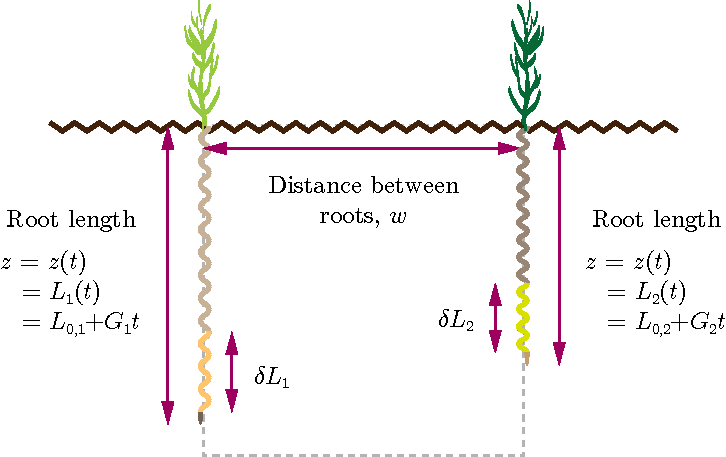
\includegraphics[scale=0.7]{Figures/Third-plot.pdf}
    \caption{Sketch of the domain for system with two plants secreting two exudates.}
    \label{fig:2roots-b}
\end{figure}

The existence of a solution is also contemplated in Section \ref{sec:Existence}.
The resulting variational formulation is 
\begin{subequations}
\label{sys:two-plants-2-weak}
\begin{align}
    \int\limits_\Omega
    A(Y_{L,1}, Y_{L,2}) \partial_t X_L v &- B(X_L, Y_{L,1}, Y_{L,2}) \partial_t Y_{L,1} v - C(X_L, Y_{L,1}, Y_{L,2}) \partial_t Y_{L,2} v \dif \mu 
    \notag
    \\
    &=
    - \int\limits_{\Gamma_{2,X}}  \alpha_2 X_L v \dif \sigma
    - \int\limits_{\Gamma_{1,X}} \alpha_1 X_L v \dif \sigma
    -\int\limits_\Omega
    (D_X \nabla X_L - \nu X_L) \cdot \nabla v  \dif \mu
    -\int\limits_\Omega g_X v \dif \mu,
    \\
    %
    \int\limits_\Omega (\theta + b_{Y,1}) \partial_t Y_{L,1} v \dif \mu  &=
    \int\limits_{\Gamma_{1,1,Y}} F_{Y,1,1} v \dif\sigma
    + \int\limits_{\Gamma_{1,2,Y}} F_{Y,1,2} v \dif\sigma
    -\int\limits_\Omega (D_{Y,1} \nabla Y_{L,1} - \nu Y_{L,1}) \cdot \nabla v \dif\mu - \int\limits_\Omega g_{Y,1} v \dif\mu,
    %
    \\
    \int\limits_\Omega (\theta + b_{Y,2}) \partial_t Y_{L,2} v \dif\mu  &=
    \int\limits_{\Gamma_{2,1,Y}} F_{Y,2,1} v \dif\sigma
    +\int\limits_{\Gamma_{2,2,Y}} F_{Y,2,2} v \dif\sigma - 
    \int\limits_\Omega (D_{Y,2} \nabla Y_{L,2} - \nu Y_{L,2}) \cdot \nabla v \dif\mu - \int\limits_\Omega g_{Y,2} v \dif\mu.
\end{align}
\end{subequations}
Here the sub subsets of \(\Gamma\) are defined implicitly by conditions \eqref{bounday-two-two}.

The discretisation of \eqref{sys:two-plants-2-weak} is similar to the one of \eqref{sys:two-plants-1-weak}. Again, its non-dimensionalisation follows a similar scheme.








%\newpage
%%%%%%%%%%%%%%%%%%%%%%%%%%%%%%%%%%%%%%%%%
%%%%%%%%%%%%%%%%%%%%%%%%%%%%%%%%%%%%%%%%%
\subsection{Scaling}

Similarly as we did in Section \ref{2-Base-Scaling}, 
we will scale the variables of the model appropriately. Again, we introduce the following relations
\[
    r = \varepsilon_r \hat{r} + a,
    \qquad
    z = \varepsilon_z \hat{z},
    \qquad
    t = \varepsilon_t \hat{t},
    \qquad
    X_L = \varepsilon_x \hat{x},
    \qquad
    Y_{L,1} = \varepsilon_{1,y} \hat{y}_1,
    \qquad
    Y_{L,2} = \varepsilon_{2,y} \hat{y}_2;
\]
where \( \varepsilon_r, \varepsilon_z, \varepsilon_t, \varepsilon_x, \varepsilon_{1,y}\), and \(\varepsilon_{2,y}\) are scaling constants to be determined, and \(\hat{r}, \hat z, \hat t, \hat x, \hat y_1\), and \(\hat y_2\) are non-dimensional variables.
Again we get the relations \(X_L(r,z) = \varepsilon_x \hat{x} (\varepsilon_r \hat r + a, \varepsilon_z \hat z) = \varepsilon_x \hat{x} \big( \varepsilon_r^{-1} (r-a) , \varepsilon_z^{-1} z\big) \), \(Y_{L,1} (r,z) = \varepsilon_{1,y} \hat{y}_1 \big( \varepsilon_r^{-1} (r-a), \varepsilon_z^{-1} z \big)\), and \(Y_{L,2} (r,z) = \varepsilon_{2,y} \hat{y}_2 \big( \varepsilon_r^{-1} (r-a), \varepsilon_z^{-1} z \big)\). Again the gradient operator is also scaled as
\[
    \nabla X_L =
    \begin{pmatrix}
        \nicefrac{1}{\varepsilon_r} & 0 \\
        0 & \nicefrac{1}{\varepsilon_z}
    \end{pmatrix}
    \hat{\nabla} \varepsilon_x \hat{x},
    \qquad \text{with} \qquad
    \hat{\nabla} = 
    \begin{pmatrix}
        \pd{ }{\hat r}
        &
        \pd{ }{\hat z}
    \end{pmatrix}^\top .
\]
For ease of presentation, we will separate the derivation into two parts. First, we will find the non-dimensionalised version of the differential equations. Here the choice of the scaling will not be explicit. This changes in the second part, where we present a scaled version of the boundary and initial conditions.

%%%%%%%%%%%%%%%%%%%%%
%%%%%%%%%%%%%%%%%%%%%
%%%%%%%%%%%%%%%%%%%%%
\subsubsection{Scaled differential equations}

The scaled equations can be found following the same steps as before. First consider the quantities
\begin{subequations}
\label{eq:generalised-x_t-parts}
\begin{align}
    \left( \theta + \frac{b_X}{1 + \kappa_{X,1} b_{X} Y_{L,1} + \kappa_{X,2} b_{X} Y_{L,2}} \right) \partial_t X_L &= \frac{\varepsilon_x}{\varepsilon_t} \left( \theta + \frac{b_X}{1 + \varepsilon_{1,y} \kappa_{X,1} b_{X} \hat{y}_1 + \varepsilon_{2,y} \kappa_{X,2} b_{X} \hat{y}_2 } \right)  \pd{\hat{x}}{\hat{t}}
    \\
    \frac{\kappa_{X,1} b_X^2 X_L}{\big(1 + \kappa_{X,1} b_{X} Y_{L,1} + \kappa_{X,2} b_{X} Y_{L,2} \big)^2} \partial_t Y_{L,1} 
    &=
    \frac{\varepsilon_x}{\varepsilon_t} \frac{\varepsilon_{1,y} \kappa_{X,1} b_X^2 \hat{x}}{\big(1+ \varepsilon_{1,y} \kappa_{X,1} b_X \hat{y}_1 + \varepsilon_{2,y} \kappa_{X,2} b_X \hat{y}_2 \big)^2} \pd{\hat y_1}{\hat t}
    \\
    \frac{ \kappa_{X,2} b_X^2 X_L }{\big(1 + \kappa_{X,1} b_X Y_{L,1} + \kappa_{X,2} b_X Y_{L,2}\big)^2} \partial_t Y_{L,2}
    &=
    \frac{\varepsilon_x}{\varepsilon_t} \frac{\varepsilon_{2,y} \kappa_{X,2} b_X^2 \hat{x}}{\big(1+ \varepsilon_{1,y} \kappa_{X,1} b_X \hat{y}_1 + \varepsilon_{2,y} \kappa_{X,2} b_X \hat{y}_2 \big)^2} \pd{\hat y_2}{\hat t}
\end{align}
\end{subequations}

We know that a linear combination of these forms \eqref{eq:generalised-x_t}, from where the term \(\nabla \cdot (D_X \nabla X_L - \nu X_L)\) follows \eqref{eq:divergence-non-dimen-x}.
Proceed to define the scaled constants and vector
\[
    \hat{\kappa}_{X,1} = \varepsilon_{1,y} \kappa_{X,1},
    \qquad
    \hat{\kappa}_{X,2} = \varepsilon_{2,y} \kappa_{X,2},
    \qquad
    \hat{\nu} = 
    \begin{pmatrix}   \hat{\nu}_r    &    \hat{\nu}_z    \end{pmatrix}^\top
    =
    \nu \varepsilon_t
    \begin{pmatrix}    {\varepsilon_r}^{-1}    &    {\varepsilon_z}^{-1}
    \end{pmatrix}^\top ,
\]
define the matrix
\[
    \hat{D}_x = 
    \begin{pmatrix}
         \hat{D}_{X,r} & 0 
         \\
        0 &  \hat{D}_{X,z}
    \end{pmatrix}
    =
    D_X \varepsilon_t
    \begin{pmatrix}
         \varepsilon_r^{-2} & 0 
         \\
        0 &  \varepsilon_z^{-2}
    \end{pmatrix}
    ,
\]
and then define the non-dimensionalised quantity \( \hat{g}_X = \nicefrac{\varepsilon_t}{\varepsilon_x} g_X\). This way we get from \eqref{eq:generalised-x_t-parts} that
\begin{equation}
\begin{aligned}
    \left( \theta + \frac{b_X}{1 + \hat{\kappa}_{X,1} b_{X} \hat{y}_1 + \hat{\kappa}_{X,2} b_{X} \hat{y}_2 } \right)  \pd{\hat{x}}{\hat{t}}
    &
    -\frac{\hat{\kappa}_{X,1} b_X^2 \hat{x}}{\big(1+ \hat{\kappa}_{X,1} b_X \hat{y}_1 + \hat{\kappa}_{X,2} b_X \hat{y}_2 \big)^2} \pd{\hat y_1}{\hat t}
    \\
    &\,\,
    -\frac{\hat{\kappa}_{X,2} b_X^2 \hat{x}}{\big(1+ \hat{\kappa}_{X,1} b_X \hat{y}_1 + \hat{\kappa}_{X,2} b_X \hat{y}_2 \big)^2} \pd{\hat y_2}{\hat t}
    =
    \hat{\nabla}
    \cdot
    \left( 
        \hat{D}_x \hat{\nabla} \hat{x} - \hat{x} \hat{\nu}
    \right)
    - \hat{g}_X.
\end{aligned}
\end{equation}

Similarly, for \eqref{eq:generalised-y_1_t}, we first get the relations
\begin{subequations}
\label{eq:generalised-y_1_t-parts}
\begin{align}
    \left(\theta + \frac{b_{Y,1}}{1 + \kappa_{Y,1} b_{Y,1} X_L}\right) \partial_t Y_{L,1} 
    &= 
    \frac{\varepsilon_{1,y}}{\varepsilon_t} \left( \theta + \frac{b_{Y,1}}{1 + \varepsilon_{x} \kappa_{Y,1} b_{Y,1} \hat{x} } \right)  \pd{\hat{y}_1}{\hat{t}}
    \\
    \frac{ \kappa_{Y,1} b_{Y,1}^2 Y_{L,1}}{\big(1 + \kappa_{Y,1} b_{Y,1} X_L\big)^2} \partial_t X_L
    &=
    \frac{\varepsilon_{1,y}}{\varepsilon_t}
    \frac{ \varepsilon_x  \kappa_{Y,1} b_{Y,1}^2 \hat{y}_{1}}{\big(1 + \varepsilon_x \kappa_{Y,1} b_{Y,1} \hat{x} \big)^2}
    \pd{\hat{x}}{\hat{t}}.
\end{align}
\end{subequations}
Now define
\[
    \hat{\kappa}_{Y,1} = \varepsilon_{x} \kappa_{Y,1},
    \qquad
    \hat{D}_{y,1} = 
    \begin{pmatrix}
         \hat{D}_{Y,1,r} & 0 
         \\
        0 &  \hat{D}_{Y,1,z}
    \end{pmatrix}
    =
    D_{Y,1} \varepsilon_t
    \begin{pmatrix}
         \varepsilon_r^{-2} & 0 
         \\
        0 &  \varepsilon_z^{-2}
    \end{pmatrix},
    \qquad\text{and}\qquad
    \hat{g}_{y,1} = \frac{\varepsilon_t}{\varepsilon_{1,y}} g_{Y,1}
\]
to get from \eqref{eq:generalised-y_1_t-parts} that
\begin{equation}
    \left( \theta + \frac{b_{Y,1}}{1 + \hat{\kappa}_{Y,1} b_{Y,1} \hat{x} } \right)  \pd{\hat{y}_1}{\hat{t}}
    -
    \frac{ \hat{\kappa}_{Y,1} b_{Y,1}^2 \hat{y}_{1}}{\big(1 + \hat{\kappa}_{Y,1} b_{Y,1} \hat{x} \big)^2}
    \pd{\hat{x}}{\hat{t}}
    = \hat{\nabla} \cdot (\hat{D}_{y,1} \hat{y}_1 - \hat{y}_1 \hat{\nu}) - \hat{g}_{y,1}.
\end{equation}




Finally, for \eqref{eq:generalised-y_2_t} define
\[
    \hat{\kappa}_{Y,2} = \varepsilon_{x} \kappa_{Y,2},
    \qquad
    \hat{D}_{y,2} = 
    \begin{pmatrix}
         \hat{D}_{Y,2,r} & 0 
         \\
        0 &  \hat{D}_{Y,2,z}
    \end{pmatrix}
    =
    D_{Y,2} \varepsilon_t
    \begin{pmatrix}
         \varepsilon_r^{-2} & 0 
         \\
        0 &  \varepsilon_z^{-2}
    \end{pmatrix},
    \qquad\text{and}\qquad
    \hat{g}_{y,2} = \frac{\varepsilon_t}{\varepsilon_{2,y}} g_{Y,2},
\]
from which we get
\begin{equation}
    \left(\theta + \frac{b_{Y,2}}{1 + \hat{\kappa}_{Y,2} b_{Y,2} \hat{x}}\right) \pd{\hat{y}_2}{\hat{t}}
    - 
    \frac{ b_{Y,2}^2 \hat{\kappa}_{Y,2} \hat{y}_2 }{\big(1 + \hat{\kappa}_{Y,2} b_{Y,2} \hat{x} \big)^2} \pd{\hat{x}}{\hat{t}} 
    = 
    \hat{\nabla} \cdot(\hat{D}_{y,2} \hat{\nabla} \hat{y}_{2} - \hat{y}_2 \hat{\nu}  ) - \hat{g}_{y,2}.
\end{equation}



%%%%%%%%%%%%%%%%%%%%%
\subsubsection{Scaled boundary and initial conditions}

The choice of the scaling parameters come from the boundary conditions. 



Here we will present the choice and development for the secretion of two exudates. The treatment is similar for the secretion of one. 

Again, the derivation is straightforward from the base model. First, we note that for \(X_L\) we get, for one side of the boundary, that
\[
    D_X \partial_r X_L - \nu X_L = 
    \frac{\varepsilon_r^2}{\varepsilon_t} \hat{D}_{X,r} \frac{\varepsilon_x}{\varepsilon_r} \pd{\hat{x}}{\hat{r}} - \frac{\varepsilon_r}{\varepsilon_t} \hat{\nu}_r \varepsilon_x \hat{x} = \frac{\varepsilon_r \varepsilon_x}{\varepsilon_t} \hat{\alpha}_1 \hat{x}
    \qquad \text{at } r = a = a + \varepsilon_r \hat{r}, \quad \varepsilon_z \hat{z} \in [L_1 - \delta L_{X,1}, L_1],
\]
or equivalently
\begin{subequations}
\begin{equation}
    \hat{D}_{X,r} \pd{\hat{x}}{\hat{r}} - \hat{\nu}_r \hat{x} = \hat{\alpha}_1 \hat{x}
    \qquad \text{at } \hat{r} = 0, \quad \hat{z} \in [\hat{L}_1 - \delta \hat{L}_{x,1}, \hat{L}_1];
\end{equation}
where we require \( \alpha_1 = \nicefrac{\varepsilon_r}{\varepsilon_t} \hat{\alpha}_1\), \( \hat{L}_1 = \varepsilon_z^{-1} L_1\), and \( \delta\hat{L}_{x,1} = \varepsilon_z^{-1} \delta L_{X,1}\). Similarly, the other side of the boundary follows
\begin{equation}
    \hat{D}_{X,r} \pd{\hat{x}}{\hat{r}} - \hat{\nu}_r \hat{x} = -\hat{\alpha}_2 \hat{x}
    \qquad \text{at } \hat{r} = 1, \quad \hat{z} \in [\hat{L}_2 - \delta \hat{L}_{x,2}, \hat{L}_2];
\end{equation}
where we have selected \( \varepsilon_r = w\), and a proper selection of constants as in the previous line.

The relationships for \(Y_{L,1}\) and \(Y_{L,2}\) are similar:
\begin{align}
    \hat{D}_{Y,1,r} \pd{\hat{y}_1}{\hat{r}} - \hat{\nu}_r \hat{y}_1 &= -\hat{F}_{1,1}(t)
    &
    \text{at } \hat{r} &= 0, \quad \hat{z} \in [\hat{L}_1 - \delta \hat{L}_{y,1,1}, \hat{L}_1],
    \\
    \hat{D}_{Y,2,r} \pd{\hat{y}_2}{\hat{r}} - \hat{\nu}_r \hat{y}_2 &= -\hat{F}_{2,1}(t)
    &
    \text{at } \hat{r} &= 0, \quad \hat{z} \in [\hat{L}_1 - \delta \hat{L}_{y,2,1}, \hat{L}_1],
    \\
    \hat{D}_{Y,1,r} \pd{\hat{y}_1}{\hat{r}} - \hat{\nu}_r \hat{y}_1 &= \hat{F}_{1,2}(t)
    &\text{at } \hat{r} &= 1, \quad \hat{z} \in [\hat{L}_2 - \delta \hat{L}_{y,1,2}, \hat{L}_2],
    \\
    \hat{D}_{Y,2,r} \pd{\hat{y}_2}{\hat{r}} - \hat{\nu}_r \hat{y}_2 &= \hat{F}_{2,2}(t)
    &\text{at } \hat{r} &= 1, \quad \hat{z} \in [\hat{L}_2 - \delta \hat{L}_{y,2,2}, \hat{L}_2];
\end{align}
\end{subequations}
where appropriate quantities are selected. For instance \( \hat{F}_{1,1} = \frac{\varepsilon_t}{\varepsilon_r \varepsilon_{1,y}} F_{Y,1,1} \).

For the other scaling parameters, notice that if we again pick \( \varepsilon_z = L_{t_{\max}}\), again \(\hat z \) will be in the range \( [0,1]\) (or \([0,-1]\) when growth is modelled downwards). 
This choice implies that \( \max_t\{|\hat{L}_1|,|\hat{L}_2|\}\) should be \(1\), where we have
\begin{align}
    \hat{L}_1 &= \hat{L}_1(\hat t) = \frac{1}{\varepsilon_z} ( L_{1,0} + G_1 \varepsilon_t \hat t )
    = \hat{L}_{1,0} + \hat{G}_1 \hat t,
    \qquad 
    \hat{L}_{1,0} = \varepsilon^{-1}_z L_{1,0},
    \qquad
    \hat{G}_1 = \varepsilon_t \varepsilon_z^{-1} G_1,
    \\
    \hat{L}_2 &= \hat{L}_2(\hat t) = \frac{1}{\varepsilon_z} ( L_{2,0} + G_2 \varepsilon_t \hat t )
    = \hat{L}_{2,0} + \hat{G}_2 \hat t,
    \qquad 
    \hat{L}_{2,0} = \varepsilon^{-1}_z L_{2,0},
    \qquad
    \hat{G}_2 = \varepsilon_t \varepsilon_z^{-1} G_2;
\end{align}
and we can further select \( \varepsilon_t = t_{\max}\) to finally have \( \hat t\) in the range \( [0,1]\). As a result, we have selected scaling parameters such that the system of partial differential equations is defined in either \( [0,1]^3\) or \([0,1]\times [0,-1] \times [0,1]\).
%
Lastly, the initial conditions are scaled as \( (\hat{x}_0,\hat{y}_{1,0},\hat{y}_{2,0} ) = (\varepsilon_x^{-1} X^0_L, \varepsilon_{1,y}^{-1} Y^0_{L,1}, \varepsilon_{2,y}^{-1} Y^0_{L,2}) \). 


Observe that again we can use parameters \(\varepsilon_x\), \(\varepsilon_{1,y}\), and \(\varepsilon_{2,y}\) to calibrate the effects of \( \hat{x}\) and \(\hat{y}\) in all of the nonlinear terms in the above equations.

\newpage
%%%%%%%%%%%%%%%%%%%%%%%%%%%%%%%%%%%%%%%%%%%%%%%%%%%%%%%%%%%%%%%%%%%%%%%%%%%
%%%%%%%%%%%%%%%%%%%%%%%%%%%%%%%%%%%%%%%%%%%%%%%%%%%%%%%%%%%%%%%%%%%%%%%%%%%
%%%%%%%%%%%%%%%%%%%%%%%%%%%%%%%%%%%%%%%%%%%%%%%%%%%%%%%%%%%%%%%%%%%%%%%%%%%

\section{Results of the extended model}
In order to solve the system numerically, we will use the open-source computing platform
FEniCS, a framework for PDE modeling, continuum mechanics, and physics simulations.
FEniCS enables users to translate the mathematical problem into Python code and solve it
efficiently using the finite element method. The main benefits of this software are that the code
is close to the mathematical formulation and that the implementation of the model does not
get much more difficult as the complexity of the model increases.
% \begin{itemize}
%     \item mention negative values at some point in the simulation (numeric errors?)
% \end{itemize}

\textcolor{red}{Explain how this is implemented in the code (linearisation, first solve for Y1, Y2, then for X), simplifying assumptions?}


\subsection{Parameters for barley-tobacco combination}
In this section, we discuss the selection of parameters in Table \ref{t:Second-model-params} for an approximate model of root dynamics between barley and tobacco plants.

\begin{table}[!htb]
\begin{center}
% \caption{Table of parameters with their meanings and values, plant 1 (LHS) is barley, plant 2 (RHS) is tobacco, component $X$ is phosphate, $Y_1$ is phytase, and $Y_2$ is citrate.}
\fontsize{9.5}{7}\selectfont
\setlength{\tabcolsep}{5.pt}
\def\arraystretch{2.0}
\begin{tabular}{lll}
\toprule
    \bf Symbol & \multicolumn{1}{l}{\bf Meaning} & \bf Value
    %
    \\ \midrule
    $\theta$ & Solution volume fraction & 0.2 -- 0.3 \\
    $f$ & Diffusion impedance factor & 0.5 \\ 
    $\rho$ & Soil bulk density & 1.2 kg/dm$^{-3}$ \\
    $D_{LX} $ & Diffusion coefficient of phosphate in free solution & $7-9 \times 10^{-8}$ dm$^2$ s$^{-1}$ \\  
	$D_{LY,1}$ &  Diffusion of phytase in free solution & $3.5 - 4.5 \times 10^{-8}$ dm$^2$ s$^{-1}$ \\   
	$D_{LY,2}$ & Diffusion of citrate in free solution & $2.1 \times 10^{-8}$ dm$^2$ s$^{-1}$ \\
	$\nu$ & Water flux & $1 \times 10^{-6}$ dm s$^{-1}$\\
	$g_X$ & Function for phosphate immobilisation & 0 \\
	$g_{Y,1}$ & Function for phytase decomposition & 0 \\
	$g_{Y,2}$ & Function for citrate decomposition & $\frac{\rho V_{max} Y_{L,2} }{K_M + Y_{L,2} }$ where $V_{max} = 0$ or $V_{max} = 2.5 \times 10^{-9}$ mol kg$^{-1}$ s$^{-1}$, \\
	 & & $K_M=10^{-8}$ M \\
	$b_X$ & Phosphate buffer power & 300 -- 2200 \\
	$b_{Y,1}$ & Phytase buffer power & 1 \\
	$b_{Y,2}$ & Citrate buffer power & 1 \\
	$\kappa_{X,1}$ & Phosphate - phytase interaction coefficient & 18.43 dm$^3$ mol$^{-1}$ \\
	$\kappa_{X,2}$ & Phosphate - citrate interaction coefficient & $92.16$ dm$^3$ mol$^{-1}$ \\
	$\kappa_{Y,1}$ & Phytase - phosphate interaction coefficient & 0 \\
	$\kappa_{Y,2}$ & Citrate - phosphate interaction coefficient & 0 \\ 
	$\alpha_1 $ & Phosphate absorbing power of root of barley & ? $1.5 \times 10^{-4} - 1.5 \times 10^{-3} $ dm s$^{-1}$ OR? $5.6 \times 10^{-3}$ dm s$^{-1}$\\
	$\alpha_2 $ & Phosphate absorbing power of root of tobacco & ?$5.6 \times 10^{-3}$ dm s$^{-1}$\\
	$F_{Y,1,1} $ & Rate of phytase exudation in barley & $2.466 \times 10^{-11} - 2.503 \times 10^{-10}$  mol dm$^{-2}$ s$^{-1}$ \\
	$F_{Y,2,1} $ & Rate of citrate exudation in barley & $1.097 \times 10^{-12} - 1.006 \times 10^{-9}$ mol dm$^{-2}$ s$^{-1}$ \\
	$F_{Y,1,2} $ & Rate of phytase exudation in tobacco &  $1.316 \times 10^{-6}$ mol dm$^{-2}$ s$^{-1}$ \\
	$F_{Y,2,2} $ & Rate of citrate exudation in tobacco &  $2.722 \times 10^{-6}$ mol dm$^{-2}$ s$^{-1}$ \\
	$L_1$ & Barley root length & increases at rate $G_1 = 0.1728$ dm day$^{-1}$ \\
	$L_2$ & Tobacco root length & increases at rate $G_2 = 0.2$ dm day$^{-1}$\\
	$\delta L_{X,1}$ & Length of phosphate uptake zone at barley & $L_1$\\
	$\delta L_{Y,1,1}$ & Length of phytase secretion zone at barley & 0.2 dm \\
	$\delta L_{Y,1,2}$ & Length of citrate secretion zone at barley & 0.2 dm\\
	$\delta L_{X,2}$ & Length of phosphate uptake zone at tobacco & $L_2$ \\
	$\delta L_{Y,1,2}$ &  Length of phytase secretion zone at tobacco & 0.2 dm \\
	$\delta L_{Y,2,2}$ &  Length of citrate secretion zone at tobacco & 0.2 dm \\
	$a$ & Root radius of barley & 0.05 dm \\
	$w$ & Distance between the roots & varied \\
\bottomrule

\end{tabular}
% \label{t:Second-model-params}
\caption{Table of parameters with their meanings and values used for numerical experiments in this section, plant 1 (LHS) is barley, plant 2 (RHS) is tobacco, component $X$ is phosphate, $Y_1$ is phytase, and $Y_2$ is citrate. \label{t:Second-model-params}
}
\end{center}

\end{table}

\subsubsection{Soil parameters}
Similarly to the model for rice \cite{Ptashnyk-2011} which needs to be submerged in water (with $\theta=0.7$ corresponding to $70\%$ water content in soil), we choose $\theta$ in the range $0.2$ to $0.3$ which should be in accordance with real-life conditions in which tobacco and barley are cultivated, along with estimated soil bulk density $\rho=1.2$ kg/dm$^{-3}$. We keep the impedance factor the same as in \cite{Ptashnyk-2011}, i.e. $f=0.5$.

\subsubsection{Diffusion coefficients}
We take the range of phosphate diffusion in water from \cite{Ptashnyk-2010} where $D_{LX} = 9 \times 10^{-8}$ dm$^2$s$^{-1}$ and from \cite{McKayFletcher-2019} where $D_{LX} = 7 \times 10^{-8}$ dm$^2$s$^{-1}$. In \cite{McKayFletcher-2019} we also have citrate diffusion in free solution $D_{LY,2} = 2.1 \times 10^{-8}$ dm$^2$s$^{-1}$. We estimate phytase diffusion to be half of citrate diffusion as its molecules are bigger so it might diffuse more slowly. Diffusion of the micronutrients in soil is calculated as $D_X = D_{LX}f\theta$, $D_{Y,1} = D_{LY,1}f\theta$, and $D_{Y,2} = D_{LY,2}f\theta$. In the table we also state the value for water flux coefficient $\nu$, however, experiments in \cite{Ptashnyk-2011} shown that the value of this coefficient doesn't have much impact on the dynamics so we don't include it in the simulations.

\subsubsection{Parameters for sorption, mutual interaction, and decomposition}
From the derivation of the extended model we recall that the phosphate buffer power is $b_X = \beta_1 / \beta_2$, where $\beta_1$, $\beta_2$ are parameters for adsorption and desorption to and from soil particles, respectively. The typical range for $b_X$ is taken from \cite{Ptashnyk-2010}. For further derivation we take $\beta_1$, $\beta_2$ from \cite{Ptashnyk-2010} where $\beta_1 = 3.7 \times 10^{-6}$ s$^{-1}$, $\beta_2 = 4.68 \times 10^{-9}$ s$^{-1}$. For simplicity we assume $b_{Y,1}=b_{Y,2} = 1$. The parameter for $X-Y_2$ interaction is $\kappa_{X,2} = \beta_4 / \beta_1$ where $\beta_4$ is phosphate enhanced desorption from soil solid due to absorbed citrate. The value $\beta_4 = 3.41 \times 10^{-4}$ is from \cite{McKayFletcher-2019} and it gives us $\kappa_{X,2} = 92.16$ dm$^3$ mol$^{-1}$. We estimate the coefficient for $X-Y_1$ interaction, $\kappa_{X,1}$, to be 5-fold smaller than $\kappa_{X,2}$. Furthermore, we consider the parameters for interaction of the exudates with phosphate ($\kappa_{Y,1}$ and $\kappa_{Y,2}$) to be negligible as the amount the exudates reacting with the soil is much larger than the amount of phosphate taken by the roots. 

Similarly to \cite{Ptashnyk-2011}, we assume that there are no reactions in the soil that involve decomposition of phosphate, i.e. $g_X = 0$. For the decomposition of citrate we might consider a Michaelis-Menten-type term $g_{Y,2} = V_{max} Y_{L,2} / (K_M + Y_{L,2})$, however, sorption of citrate to soil particles causes up to 99\% reduction in biodegradation rate \cite{McKayFletcher-2019}. We therefore choose $V_{max} = 0$ and experiment with non-zero values similar to those in \cite{Ptashnyk-2011}. For phytase we also set $g_{Y,2} = 0$ since we assume no microbial consumption of this nutrient.

\subsubsection{Absorption power and exudation rates}
The coefficients for exudation rates in barley are taken from \cite{Ruiz-2020} \textcolor{red}{Add conversion details (from nkat)?} Tobacco exudation rates were obtained from \cite{giles_george} where we tried to estimate the root surface by using root radius being half of barley root radius (i.e. $a_2 = 2.5 \times 10^{-3}$) and the length of the root 100 dm, approximating the root(s) as a cylinder. However, this way both $F_{Y,1,2}$ and $F_{Y,2,2}$ were of order $10^{-6}$ which is much larger than the order of magnitude of $F_{Y,1,1}$ and $F_{Y,2,1}$ being $10^{-10}$. The relatively large exudation rates caused issues in the numerical simulations (the values of phosphate were blowing up). We therefore considered all of the exudation rates in the system to be of order $10^{-10}$, i.e. we multiplied the calculated values for $F_{Y,1,2}$ and $F_{Y,2,2}$ by $10^{-4}$.

\subsubsection{Geometry of the domain}
The domain's main axes are $r$ (horizontal) and $z$ (vertical), see Fig. \ref{fig:2roots-b}. For the simulations we chose the distance between the two roots (i.e. the width of the simulation window) to be $w = 0.04$ dm. The height of the simulation window is chosen to be the length of one of the roots after 3-day growth. In both plants, phosphate is absorbed along the whole length of root. For the exudation we choose to locate the 2cm long exudation zone to be 2cm behind the root tip (i.e. before the root cap).

% \begin{table}[!htb]
% \begin{center}
% % \caption{Table of parameters with their meanings and values, plant 1 (LHS) is barley, plant 2 (RHS) is tobacco, component $X$ is phosphate, $Y_1$ is phytase, and $Y_2$ is citrate.}
% \fontsize{9.5}{7}\selectfont
% \setlength{\tabcolsep}{5.pt}
% \def\arraystretch{2.0}
% \begin{tabular}{lll}
% \toprule
%     \bf Symbol & \multicolumn{1}{l}{\bf Meaning} & \bf Value
%     %
%     \\ \midrule
%     $\theta$ & Solution volume fraction & 0.2 -- 0.3 \\
%     $f$ & Diffusion impedance factor & 0.5 \\ 
%     $\rho$ & Soil bulk density & 1.2 kg/dm$^{-3}$ \\
%     $D_{LX} $ & Diffusion coefficient of phosphate in free solution & $7-9 \times 10^{-8}$ dm$^2$ s$^{-1}$ \\  
% 	$D_{LY,1}$ &  Diffusion of phytase in free solution & $3.5 - 4.5 \times 10^{-8}$ dm$^2$ s$^{-1}$ \\   
% 	$D_{LY,2}$ & Diffusion of citrate in free solution & $2.1 \times 10^{-8}$ dm$^2$ s$^{-1}$ \\
% 	$\nu$ & Water flux & $1 \times 10^{-6}$ dm s$^{-1}$\\
% 	$g_X$ & Function for phosphate immobilisation & 0 \\
% 	$g_{Y,1}$ & Function for phytase decomposition & 0 \\
% 	$g_{Y,2}$ & Function for citrate decomposition & $\frac{\rho V_{max} Y_{L,2} }{K_M + Y_{L,2} }$ where $V_{max} = 0$ or $V_{max} = 2.5 \times 10^{-9}$ mol kg$^{-1}$ s$^{-1}$, \\
% 	 & & $K_M=10^{-8}$ M \\
% 	$b_X$ & Phosphate buffer power & 300 -- 2200 \\
% 	$b_{Y,1}$ & Phytase buffer power & 1 \\
% 	$b_{Y,2}$ & Citrate buffer power & 1 \\
% 	$\kappa_{X,1}$ & Phosphate - phytase interaction coefficient & 18.43 dm$^3$ mol$^{-1}$ \\
% 	$\kappa_{X,2}$ & Phosphate - citrate interaction coefficient & $92.16$ dm$^3$ mol$^{-1}$ \\
% 	$\kappa_{Y,1}$ & Phytase - phosphate interaction coefficient & 0 \\
% 	$\kappa_{Y,2}$ & Citrate - phosphate interaction coefficient & 0 \\ 
% 	$\alpha_1 $ & Phosphate absorbing power of root of barley & ? $1.5 \times 10^{-4} - 1.5 \times 10^{-3} $ dm s$^{-1}$ OR? $5.6 \times 10^{-3}$ dm s$^{-1}$\\
% 	$\alpha_2 $ & Phosphate absorbing power of root of tobacco & ?$5.6 \times 10^{-3}$ dm s$^{-1}$\\
% 	$F_{Y,1,1} $ & Rate of phytase exudation in barley & $2.466 \times 10^{-11} - 2.503 \times 10^{-10}$  mol dm$^{-2}$ s$^{-1}$ \\
% 	$F_{Y,2,1} $ & Rate of citrate exudation in barley & $1.097 \times 10^{-12} - 1.006 \times 10^{-9}$ mol dm$^{-2}$ s$^{-1}$ \\
% 	$F_{Y,1,2} $ & Rate of phytase exudation in tobacco &  $1.316 \times 10^{-6}$ mol dm$^{-2}$ s$^{-1}$ \\
% 	$F_{Y,2,2} $ & Rate of citrate exudation in tobacco &  $2.722 \times 10^{-6}$ mol dm$^{-2}$ s$^{-1}$ \\
% 	$L_1$ & Barley root length & increases at rate $G_1 = 0.1728$ dm day$^{-1}$ \\
% 	$L_2$ & Tobacco root length & increases at rate $G_2 = 0.2$ dm day$^{-1}$\\
% 	$\delta L_{X,1}$ & Length of phosphate uptake zone at barley & $L_1$\\
% 	$\delta L_{Y,1,1}$ & Length of phytase secretion zone at barley & 0.2 dm \\
% 	$\delta L_{Y,1,2}$ & Length of citrate secretion zone at barley & 0.2 dm\\
% 	$\delta L_{X,2}$ & Length of phosphate uptake zone at tobacco & $L_2$ \\
% 	$\delta L_{Y,1,2}$ &  Length of phytase secretion zone at tobacco & 0.2 dm \\
% 	$\delta L_{Y,2,2}$ &  Length of citrate secretion zone at tobacco & 0.2 dm \\
% 	$a$ & Root radius of barley & 0.05 dm \\
% 	$w$ & Distance between the roots & varied \\
% \bottomrule

% \end{tabular}
% % \label{t:Second-model-params}
% \caption{Table of parameters with their meanings and values used for numerical experiments in this section, plant 1 (LHS) is barley, plant 2 (RHS) is tobacco, component $X$ is phosphate, $Y_1$ is phytase, and $Y_2$ is citrate. \label{t:Second-model-params}
% }
% \end{center}

% \end{table}

%%%%%%%%%%%%%%%%%%%%%%%%%%%%%%%%%%%%%%%%%%%%5
\subsection{Numerical experiments}
Description and analysis of the results TBD
% To try:
% \begin{itemize}
%     \item basic model (only the parameters from the table)
%     \item basic model, different distances
%     \item change buffer rates
%     \item Vmax nonzero for citrate
%     \item change interaction coefficients
%     \item change uptake power (different for each plant?)
%     \item change exudation rates
%     \item change growth rates
% \end{itemize}

% \clearpage
% \newpage

%%%%%%%%%%%%%%%%%%%%%%%%%%%%%%%%%%%%%%%%%%%
\FloatBarrier
\subsubsection{Original parameters}

\begin{figure}[!htb]
\centering
\begin{subfigure}[t]{0.3\textwidth}
    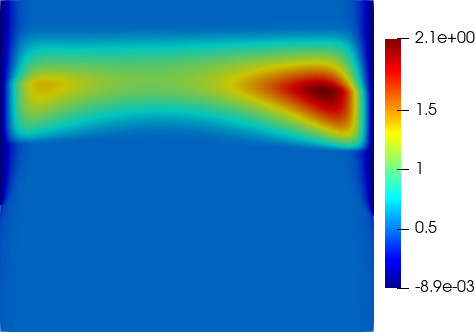
\includegraphics[trim= 100 100 70 100,width=\textwidth]{Figures/X.png}
    \caption{Phosphate ($X$)}
\end{subfigure}
\qquad
\begin{subfigure}[t]{0.3\textwidth}
    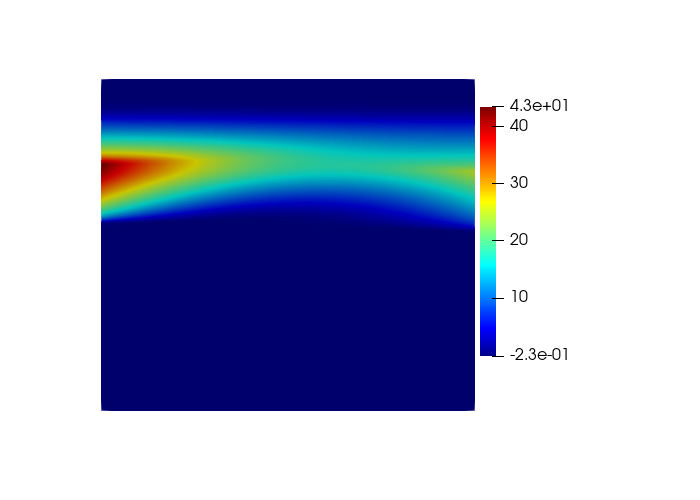
\includegraphics[trim= 100 100 70 100,width=\textwidth]{Figures/Y1.png}
    \caption{Phytase ($Y_1$)}
\end{subfigure}
\qquad
\begin{subfigure}[t]{0.3\textwidth}
    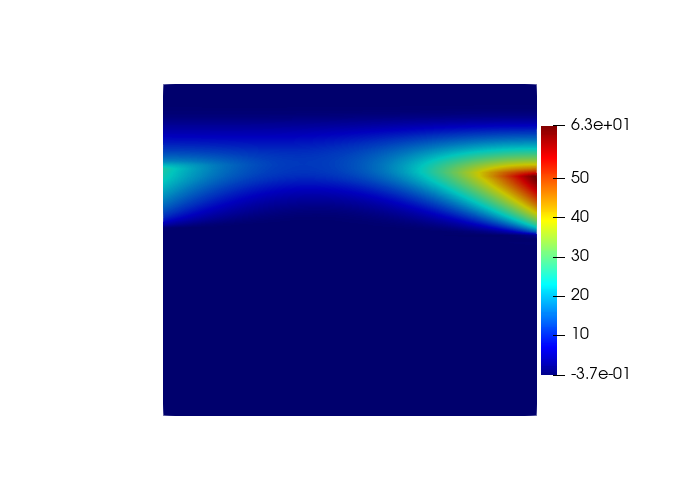
\includegraphics[trim=100 100 70 100,width=\textwidth]{Figures/Y2.png}
    \caption{Citrate ($Y_2$)}
\end{subfigure}
\caption{Concentrations of the nutrients between the two roots after 24 hours.}
\end{figure}

%%%%%%%%%%%%%%%%%%%%%%%%%%%%%%%%%%%%%%%%%%%
\FloatBarrier
\subsubsection{Citrate consumed by microbes}
\begin{figure}[!htb]
\centering
\begin{subfigure}[t]{0.45\textwidth}
    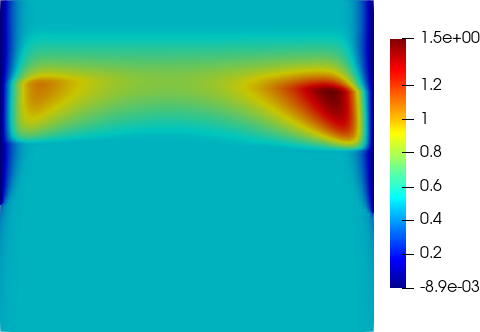
\includegraphics[trim= 100 100 60 100,width=\textwidth]{Figures/X_citrateVmaxnonzero.png}
    \caption{Phosphate ($X$)}
\end{subfigure}
\qquad
\begin{subfigure}[t]{0.45\textwidth}
    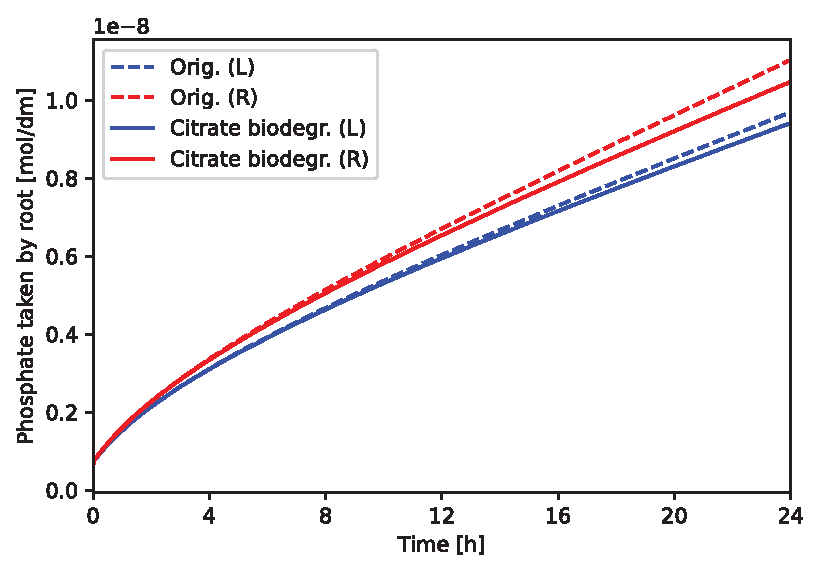
\includegraphics[width=\textwidth]{Figures/citratevmaxnonzero.eps}
    \caption{Cumulative uptake of phosphate by the left (L) and right (R) root.}
\end{subfigure}

\caption{$V_{max} = 2.5 \times 10^{-9}$ mol kg$^{-1}$ s$^{-1}$, i.e. citrate gets consumed by microbes. In (a) concentration of phosphate between the two roots after 24 hours; (b) comparison of phosphate absorbed by each of the roots with original and changed parameters.}
\end{figure}

%%%%%%%%%%%%%%%%%%%%%%%%%%%%%%%%%%%%%%%%%%%
\FloatBarrier
\subsubsection{Increased phosphate buffer power}
\begin{figure}[!htb]
\centering
\begin{subfigure}[t]{0.45\textwidth}
    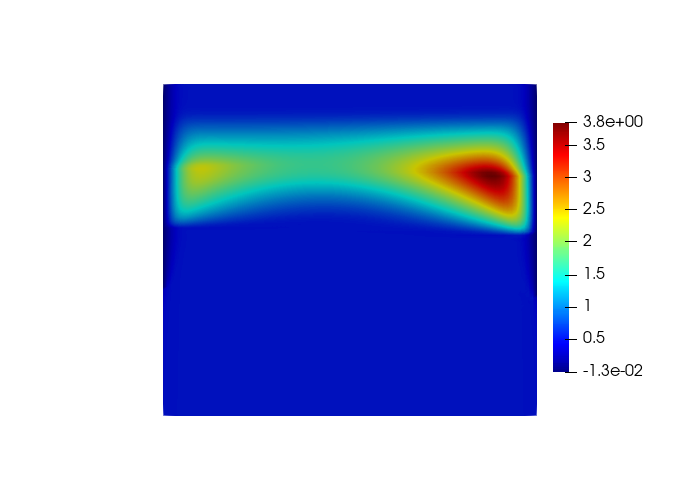
\includegraphics[trim= 100 100 60 100,width=\textwidth]{Figures/X_bXtimes2.png}
    \caption{Phosphate ($X$)}
\end{subfigure}
\qquad
\begin{subfigure}[t]{0.45\textwidth}
    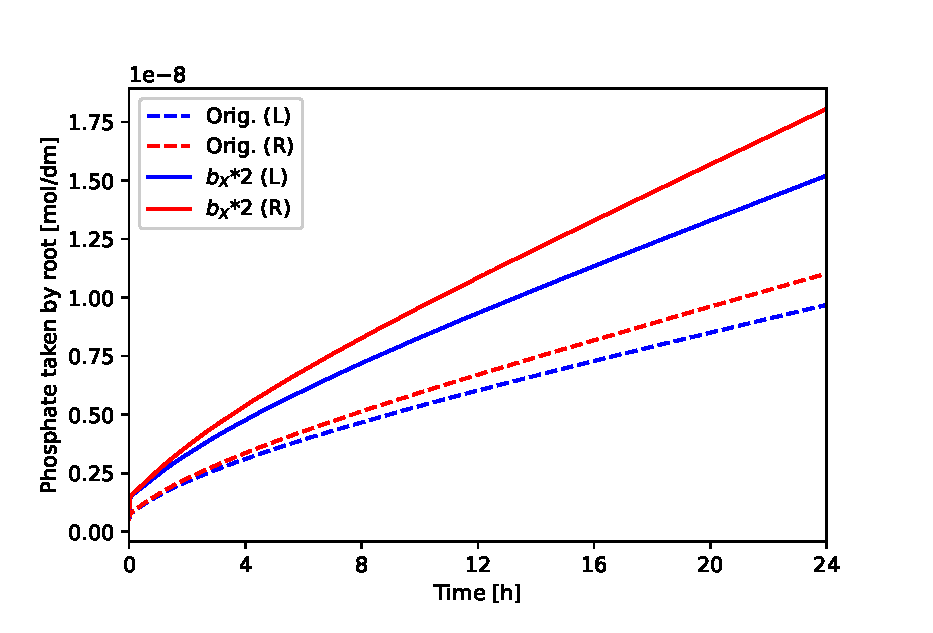
\includegraphics[width=\textwidth]{Figures/bxtimes2.eps}
    \caption{Cumulative uptake of phosphate by the left (L) and right (R) root.}
\end{subfigure}

\caption{Buffer power $b_X$ mutliplied by 2. In (a) concentration of phosphate between the two roots after 24 hours; (b) comparison of phosphate absorbed by each of the roots with original and changed parameters.}
\end{figure}

%%%%%%%%%%%%%%%%%%%%%%%%%%%%%%%%%%%%%%%%%%%
\FloatBarrier
\subsubsection{Decreased phosphate buffer power}
\begin{figure}[!htb]
\centering
\begin{subfigure}[t]{0.45\textwidth}
    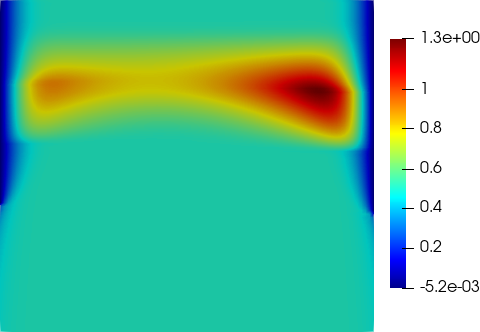
\includegraphics[trim= 100 100 60 100,width=\textwidth]{Figures/X_bXdivby2.png}
    \caption{Phosphate ($X$)}
\end{subfigure}
\qquad
\begin{subfigure}[t]{0.45\textwidth}
    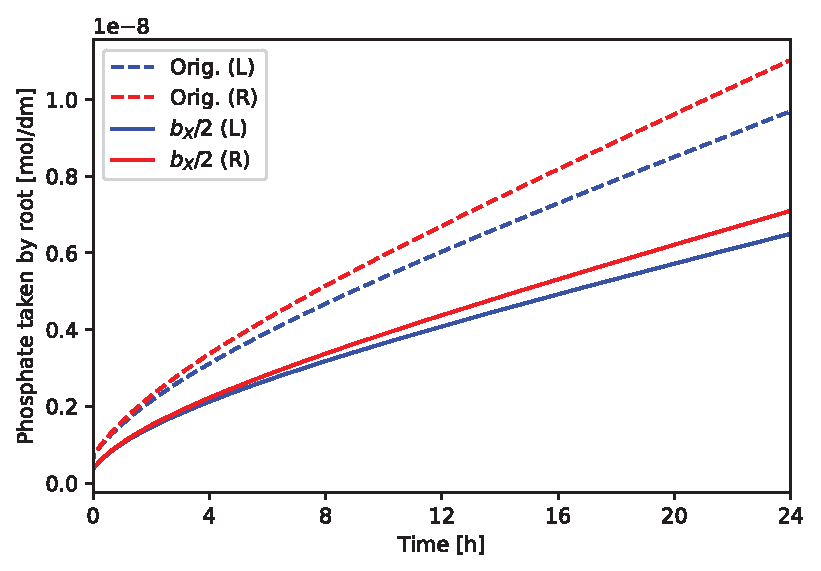
\includegraphics[width=\textwidth]{Figures/bxdivby2.eps}
    \caption{Cumulative uptake of phosphate by the left (L) and right (R) root.}
\end{subfigure}

\caption{Buffer power $b_X$ divided by 2. In (a) concentration of phosphate between the two roots after 24 hours; (b) comparison of phosphate absorbed by each of the roots with original and changed parameters.}
\end{figure}

%%%%%%%%%%%%%%%%%%%%%%%%%%%%%%%%%%%%%%%%%%%
\FloatBarrier
\subsubsection{Increased uptake power at left root}
\begin{figure}[!htb]
\centering
\begin{subfigure}[t]{0.45\textwidth}
    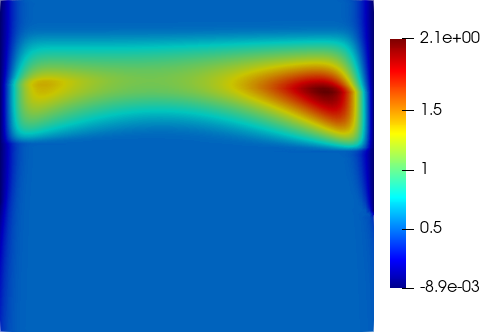
\includegraphics[trim= 100 100 60 100,width=\textwidth]{Figures/X_alpha1times10.png}
    \caption{Phosphate ($X$)}
\end{subfigure}
\qquad
\begin{subfigure}[t]{0.45\textwidth}
    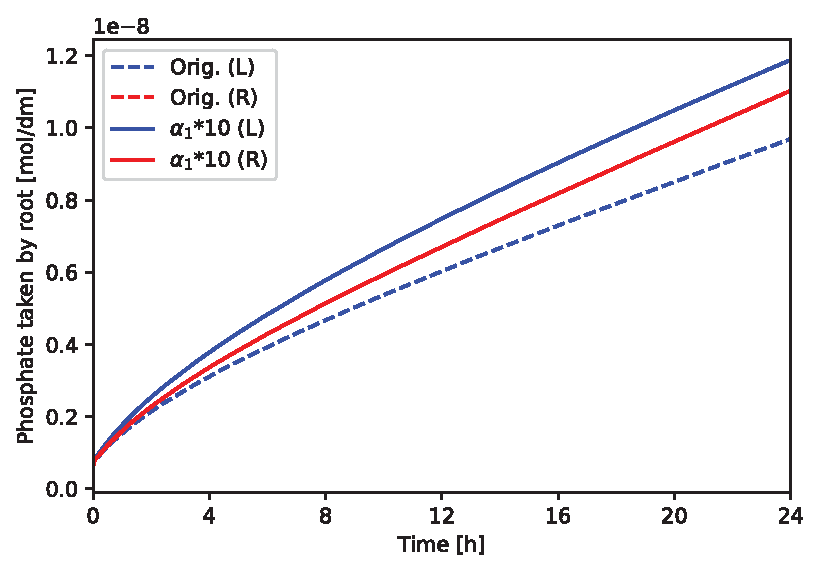
\includegraphics[width=\textwidth]{Figures/alpha1times10.eps}
    \caption{Cumulative uptake of phosphate by the left (L) and right (R) root.}
\end{subfigure}

\caption{Phosphate uptake power $\alpha_1$ multiplied by 10. In (a) concentration of phosphate between the two roots after 24 hours; (b) comparison of phosphate absorbed by each of the roots with original and changed parameters.}
\end{figure}

%%%%%%%%%%%%%%%%%%%%%%%%%%%%%%%%%%%%%%%%%%%
\FloatBarrier
\subsubsection{Decreased uptake power at left root}
\begin{figure}[!htb]
\centering
\begin{subfigure}[t]{0.45\textwidth}
    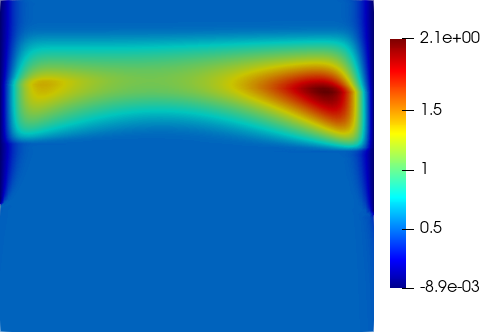
\includegraphics[trim= 100 100 60 100,width=\textwidth]{Figures/X_alpha1divby10.png}
    \caption{Phosphate ($X$)}
\end{subfigure}
\qquad
\begin{subfigure}[t]{0.45\textwidth}
    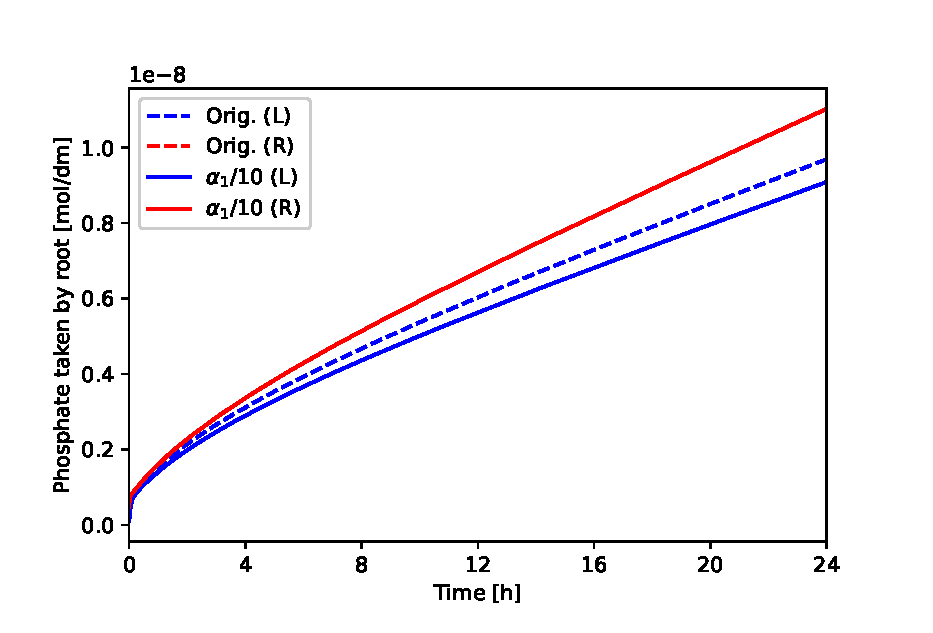
\includegraphics[width=\textwidth]{Figures/alpha1divby10.eps}
    \caption{Cumulative uptake of phosphate by the left (L) and right (R) root.}
\end{subfigure}

\caption{Phosphate uptake power $\alpha_1$ divided by 10. In (a) concentration of phosphate between the two roots after 24 hours; (b) comparison of phosphate absorbed by each of the roots with original and changed parameters.}
\end{figure}

%%%%%%%%%%%%%%%%%%%%%%%%%%%%%%%%%%%%%%%%%%%
\FloatBarrier
\subsubsection{Increase in phytase exudation rate at left root}
\begin{figure}[!htb]
\centering
\begin{subfigure}[t]{0.45\textwidth}
    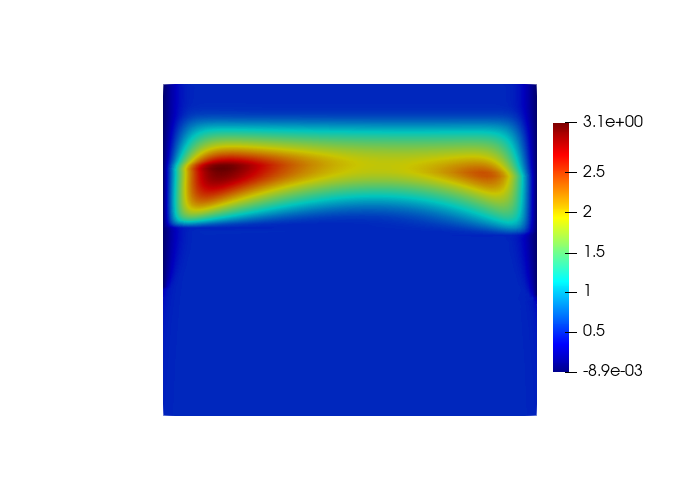
\includegraphics[trim= 100 100 60 100,width=\textwidth]{Figures/X_Fy11times10.png}
    \caption{Phosphate ($X$)}
\end{subfigure}
\qquad
\begin{subfigure}[t]{0.45\textwidth}
    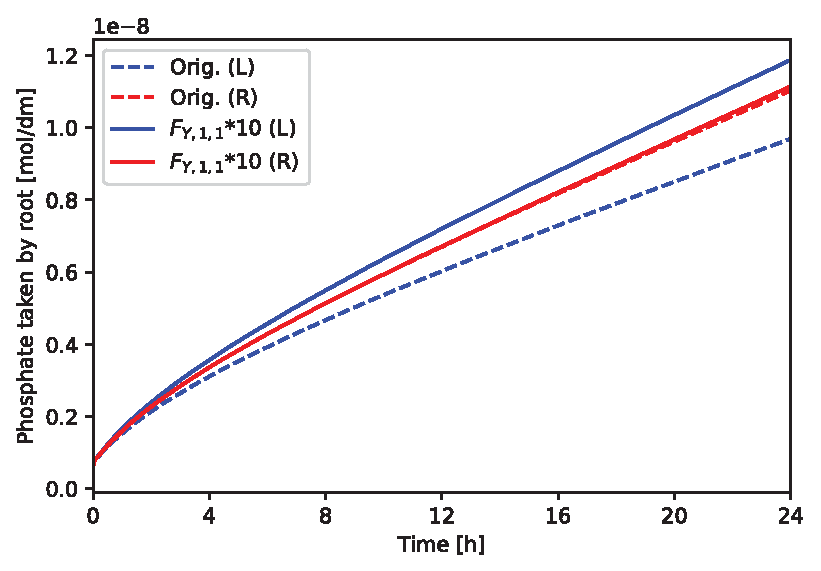
\includegraphics[width=\textwidth]{Figures/Fy11times10.eps}
    \caption{Cumulative uptake of phosphate by the left (L) and right (R) root.}
\end{subfigure}

\caption{Phytase exudation rate power $F_{Y,1,1}$ multiplied by 10. In (a) concentration of phosphate between the two roots after 24 hours; (b) comparison of phosphate absorbed by each of the roots with original and changed parameters.}
\end{figure}


\begin{figure}[!htb]
\centering
\begin{subfigure}[t]{0.45\textwidth}
    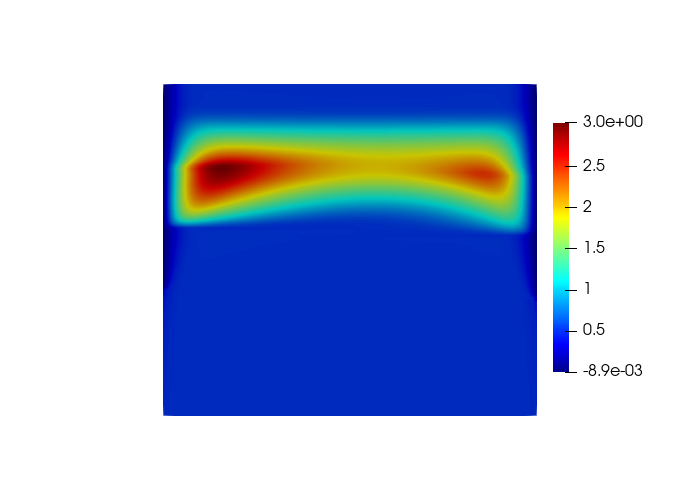
\includegraphics[trim= 100 100 60 100,width=\textwidth]{Figures/X_Fy11times10Y1up20pc.png}
    \caption{Phosphate ($X$)}
\end{subfigure}
\qquad
\begin{subfigure}[t]{0.45\textwidth}
    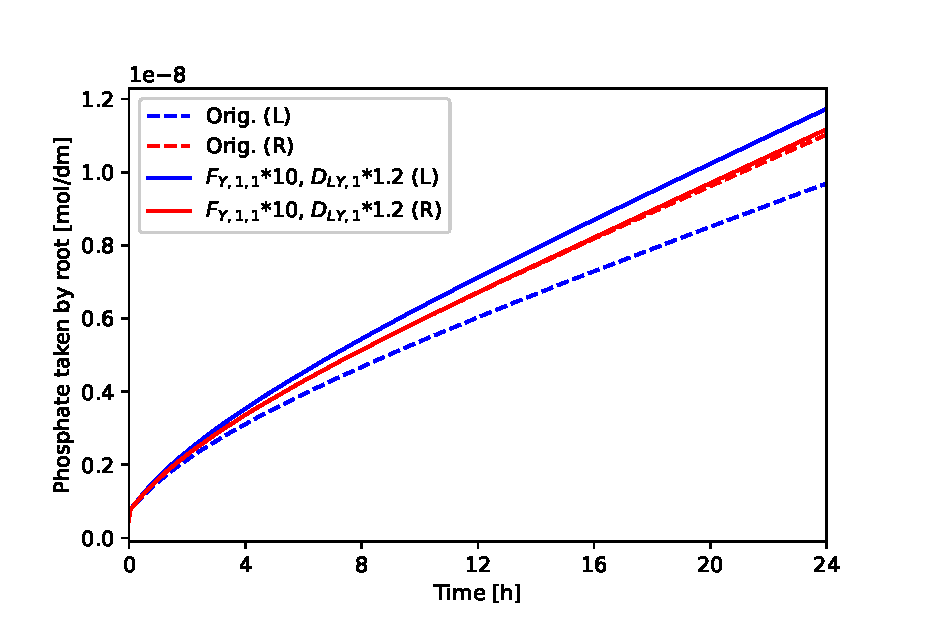
\includegraphics[width=\textwidth]{Figures/Fy11times10DY1up20pc.eps}
    \caption{Cumulative uptake of phosphate by the left (L) and right (R) root.}
\end{subfigure}

\caption{Phytase exudation rate power $F_{Y,1,1}$ multiplied by 10 combined with $20\%$ increase in diffusion of phytase $D_{LY,1}$. In (a) concentration of phosphate between the two roots after 24 hours; (b) comparison of phosphate absorbed by each of the roots with original and changed parameters.}
\end{figure}

\begin{table}[h]
\begin{center}

\fontsize{9.5}{7}\selectfont
\setlength{\tabcolsep}{5.pt}
\def\arraystretch{2.0}
\begin{tabular}{rcccc}
\toprule
 & \multicolumn{2}{c}{\textbf{Total phosphate taken by root after 24h [mol dm$^{-1}$]}} & \multicolumn{2}{c}{\textbf{Change}} \\
 \hline
  \textbf{Parameter change} & \textbf{Left root} & \textbf{Right root} & \textbf{Left root}  & \textbf{Right root}\\
 \hline 
Base parameters & 9.689e$^{-9}$ &  1.103e$^{-8}$& - &- \\
Citrate $V_{max}$ nonzero     & 9.409e$^{-9}$ & 1.047e$^{-8}$ & -2.9\% & -5.08\%\\
$b_x / 2$                     & 6.495e$^{-9}$ & 7.095e$^{-9}$ & -33.0\% & -35.68\%\\
$b_x * 2$                     & 1.521e$^{-8}$ & 1.806e$^{-8}$ & 57.0\% & 63.74\% \\
$\alpha_1 * 10$                & 1.188e$^{-8}$ & 1.103e$^{-8}$ & 22.6\% & 0.00\% \\
$\alpha_1 / 10$                & 9.087e$^{-9}$ & 1.103e$^{-8}$ & -6.2\% & 0.00\% \\
$F_{Y,1,1}*10$                & 1.187e$^{-8}$ & 1.114e$^{-8}$ & 22.5\% & 1.00\% \\
$F_{Y,1,1}*10\text{ and } D_{Y1}*1.2$ & 1.173e$^{-8}$ & 1.117e$^{-8}$ & 21.1\% & 1.27\%   \\
\bottomrule
\end{tabular}
\caption{Total phosphate absorbed in each of the roots after 24 hours and change of resulting values with respect to results obtained by using the original (base) parameters defined in Table \ref{t:Second-model-params}.}
\end{center}
\end{table}

\newpage
\clearpage

















% \newpage
% \clearpage
% \section{Figures}
% \begin{figure}[h]
%     \centering
%     \caption{Basic}
%     \begin{subfigure}[t]{\textwidth}\centering
%     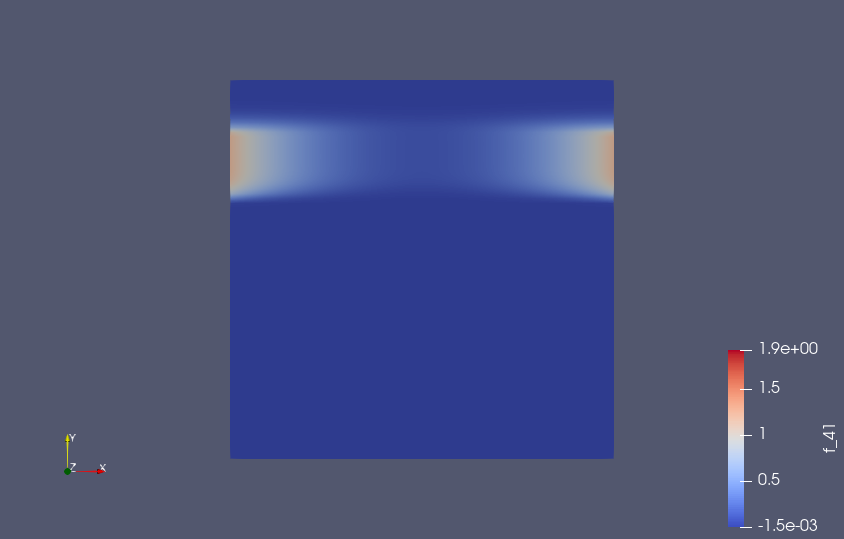
\includegraphics[width=0.6\textwidth]{Basic24DMA.png}
%     \caption{0.08 apart DMA after 24 hours}
%     \end{subfigure}
%     %
%     \begin{subfigure}[t]{\textwidth}\centering
%     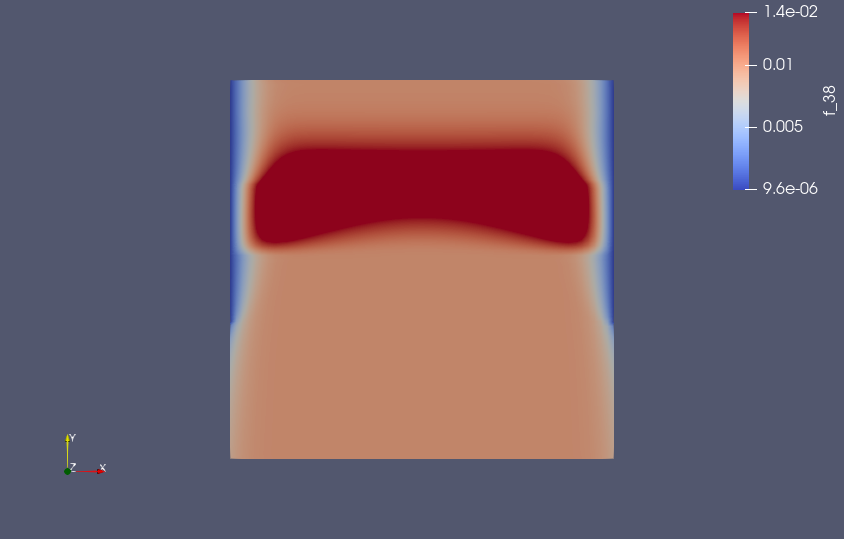
\includegraphics[width=0.6\textwidth]{Basic24Zn.png}
%     \caption{0.08 apart Zn after 24 hours}
%     \end{subfigure}
% \end{figure}

% \newpage
% \begin{figure}
%     \centering
%     \caption{Increased distance}
%     \begin{subfigure}[t]{0.45\textwidth}
%     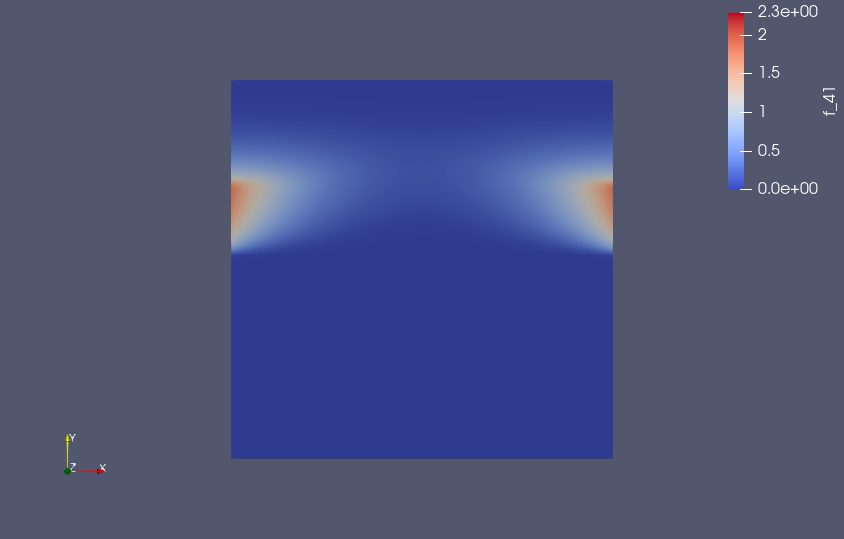
\includegraphics[width=\textwidth]{0.13ApartDMA24.png}
%     \caption{0.15 apart DMA after 24 hours}
%     \end{subfigure}
%     \begin{subfigure}[t]{0.45\textwidth}
%     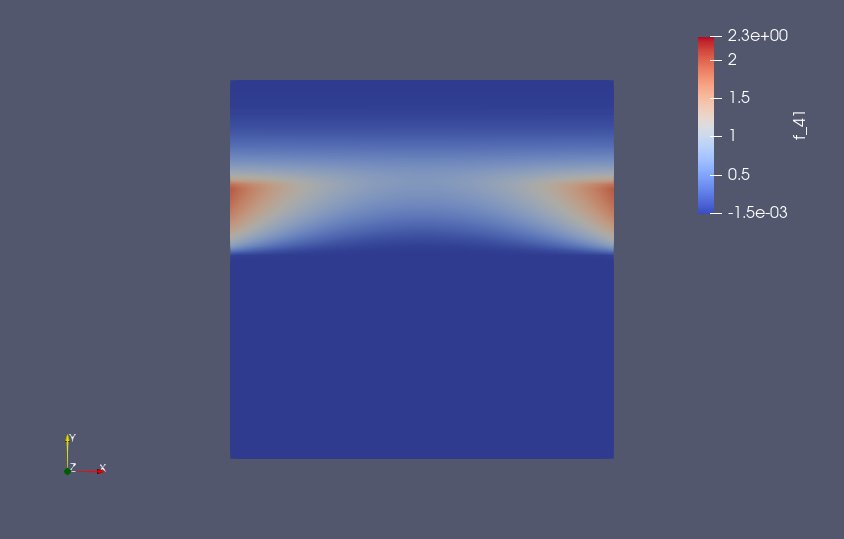
\includegraphics[width=\textwidth]{BasictoComparetoDistance.png}
%     \caption{Re-scaled basic model Zn after 24 hours for comparison}
%     \end{subfigure}
% \end{figure}
% \begin{figure}
%     \centering
%     \caption{Increased distance}
%     \begin{subfigure}[t]{0.45\textwidth}
%     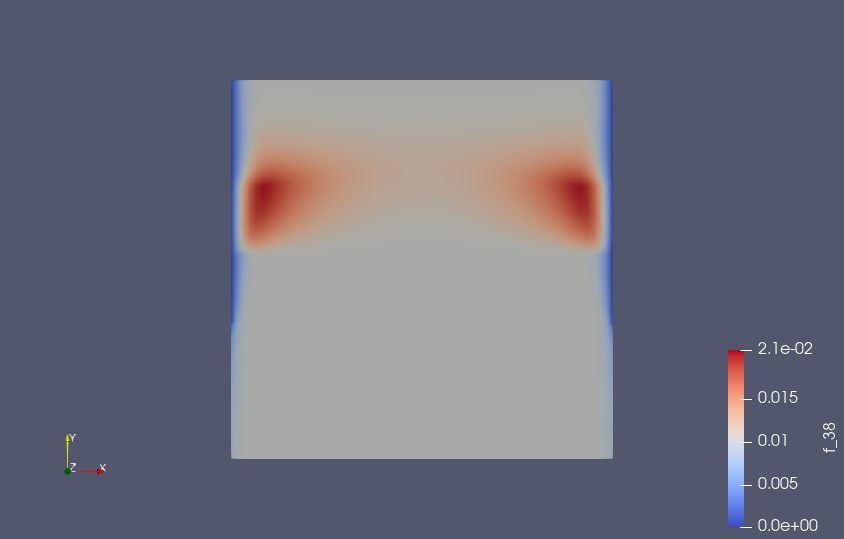
\includegraphics[width=\textwidth]{0.13ApartZn24.png}
%     \caption{0.15 apart Zn after 24 hours}
%     \end{subfigure}
%     \begin{subfigure}[t]{0.45\textwidth}
%     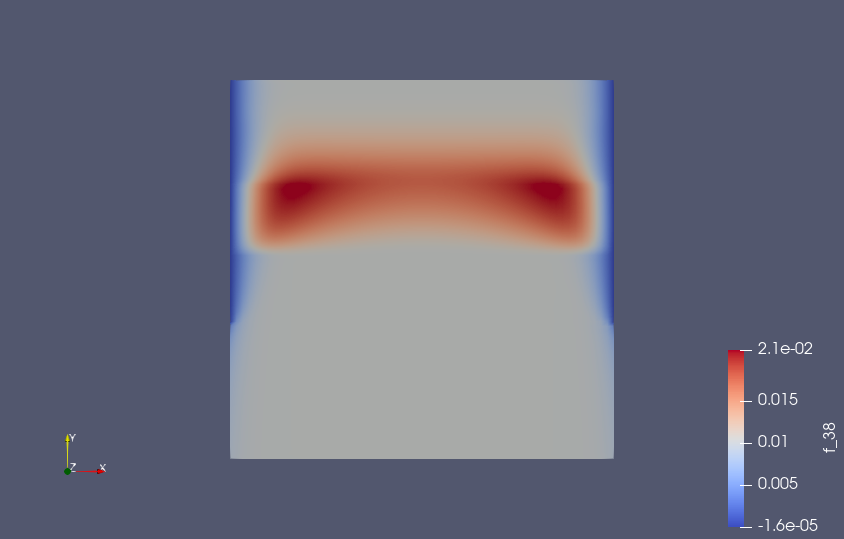
\includegraphics[width=\textwidth]{BasictoComparetoDistanceZn.png}
%     \caption{Re-scaled basic model Zn after 24 hours for comparison}
%     \end{subfigure}
% \end{figure}

% \begin{figure}
%     \centering
%     \caption{DMA increased}
%     \begin{subfigure}[t]{0.45\textwidth}
%     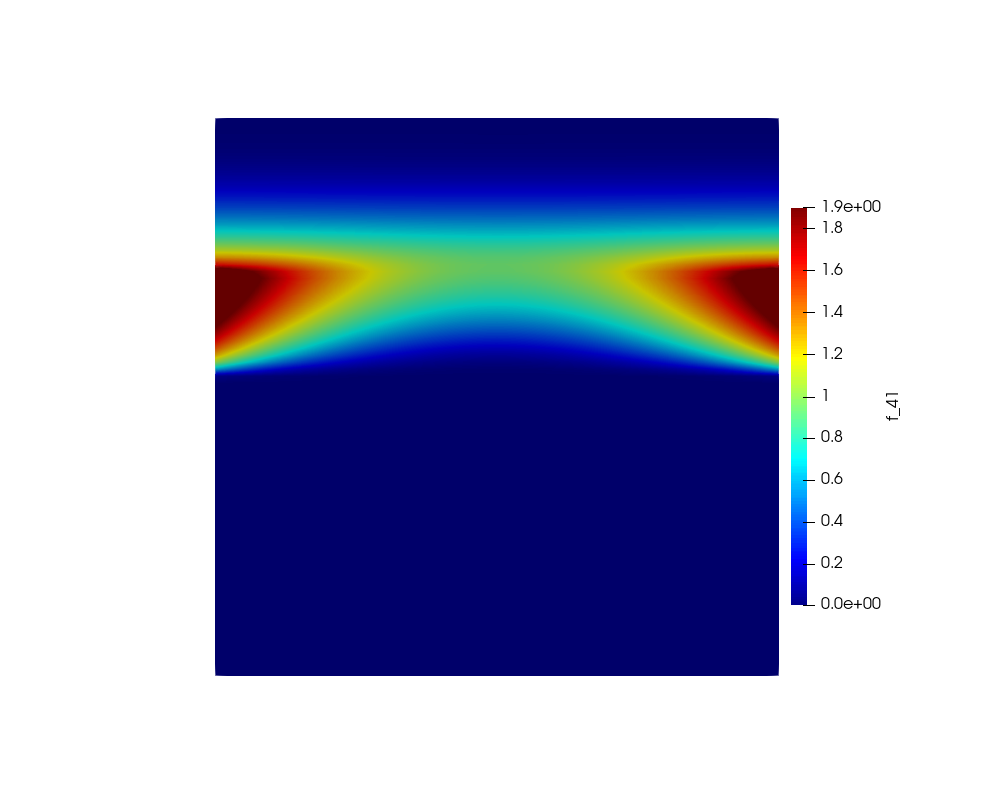
\includegraphics[width=\textwidth]{IncreasedBufferDMA24.png}
%     \caption{0.08 apart, rate of DMA exudation increased by $10^{-11}$, DMA after 24 hours}
%     \end{subfigure}
%     \begin{subfigure}[t]{0.45\textwidth}
%     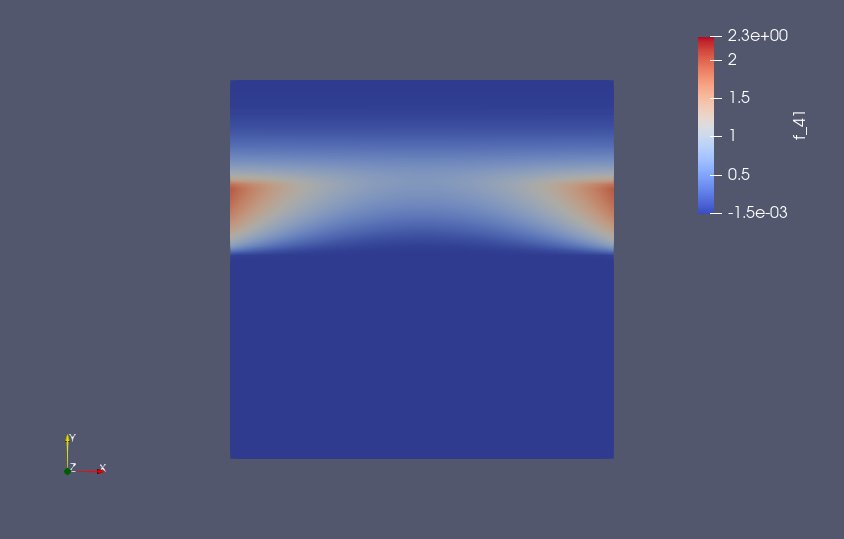
\includegraphics[width=\textwidth]{BasictoComparetoDistance.png}
%     \caption{Re-scaled basic model DMA after 24 hours for comparison}
%     \end{subfigure}
% \end{figure}
% \begin{figure}
%     \centering
%     \caption{DMA increased}
%     \begin{subfigure}[t]{0.45\textwidth}
%     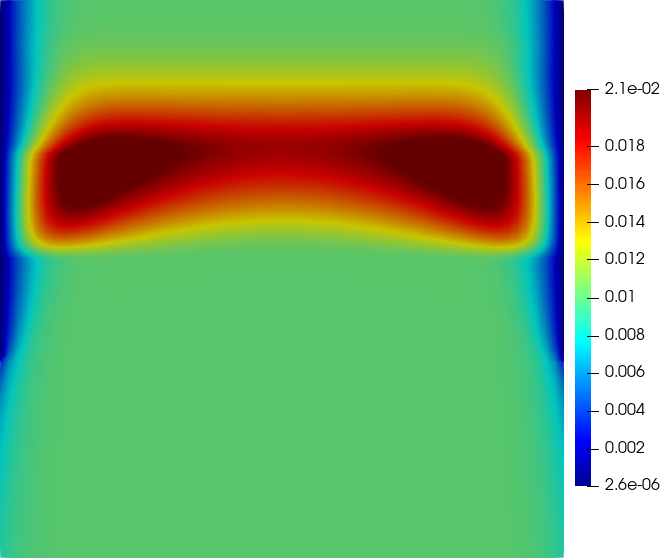
\includegraphics[width=\textwidth]{IncreasedBufferZn24.png}
%     \caption{0.08 apart, rate of DMA exudation increased by $10^{-11}$, Zn after 24 hours}
%     \end{subfigure}
%     \begin{subfigure}[t]{0.45\textwidth}
%     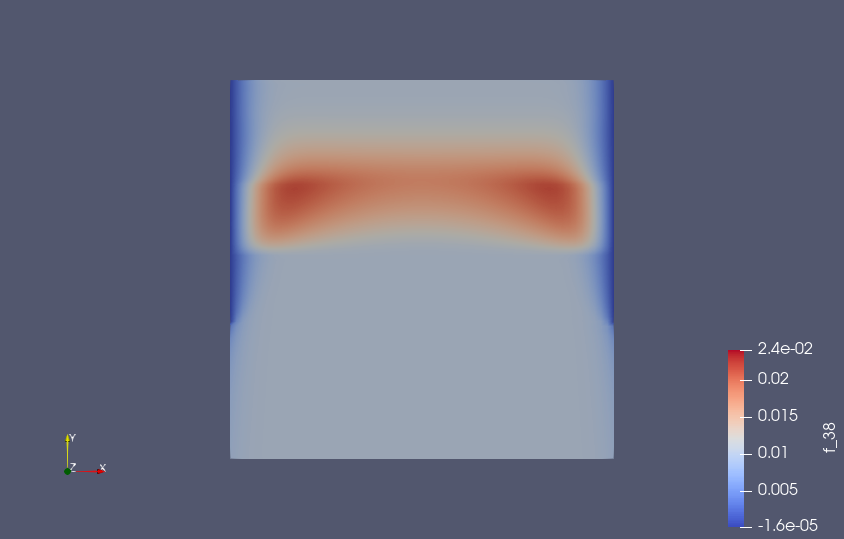
\includegraphics[width=\textwidth]{24rescaledZinc.png}
%     \caption{Re-scaled basic model Zn after 24 hours for comparison}
%     \end{subfigure}
% \end{figure}
% \begin{figure}
%     \centering
%     \caption{Distance and DMA exudation increased}
%     \begin{subfigure}[t]{0.45\textwidth}
%     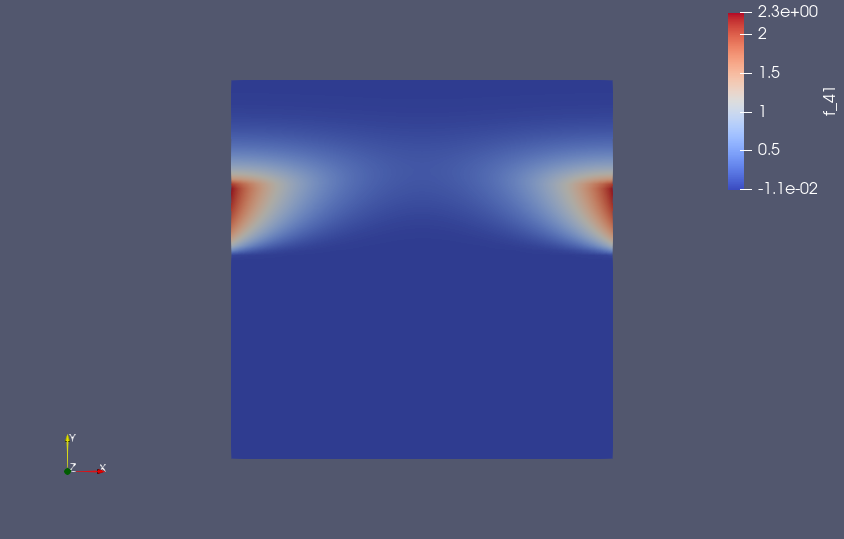
\includegraphics[width=\textwidth]{IncreasedBufferAndDistanceDMA24.png}
%     \caption{0.15 apart, rate of DMA exudation increased by $10^{-11}$, DMA after 24 hours}
%     \end{subfigure}
%     \begin{subfigure}[t]{0.45\textwidth}
%     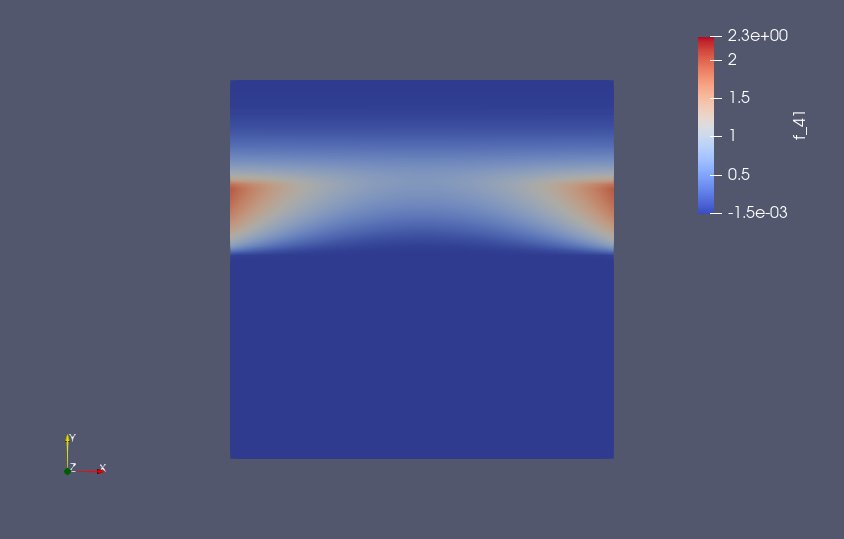
\includegraphics[width=\textwidth]{BasictoComparetoDistance.png}
%     \caption{Re-scaled basic model DMA after 24 hours for comparison}
%     \end{subfigure}
% \end{figure}
% \begin{figure}
%     \centering
%     \begin{subfigure}[t]{0.45\textwidth}
%     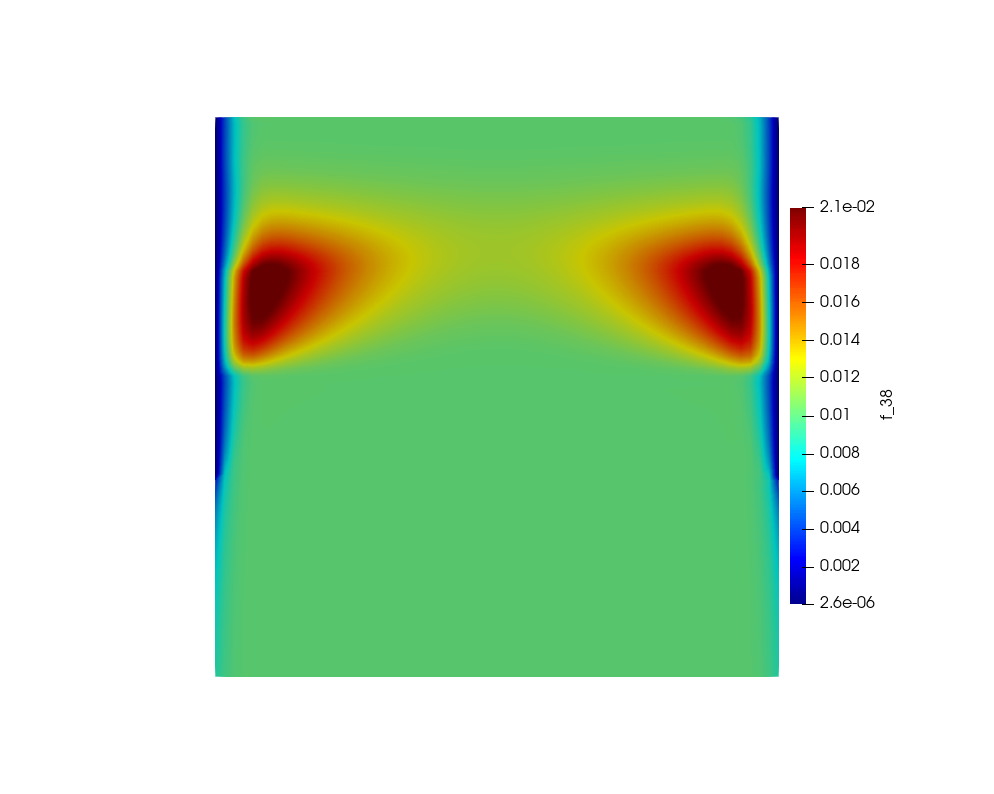
\includegraphics[width=\textwidth]{IncreasedBufferAndDistanceZn24.png}
%     \caption{0.15 apart, rate of DMA exudation increased by $10^{-11}$, Zn after 24 hours}
%     \end{subfigure}
%     \begin{subfigure}[t]{0.45\textwidth}
%     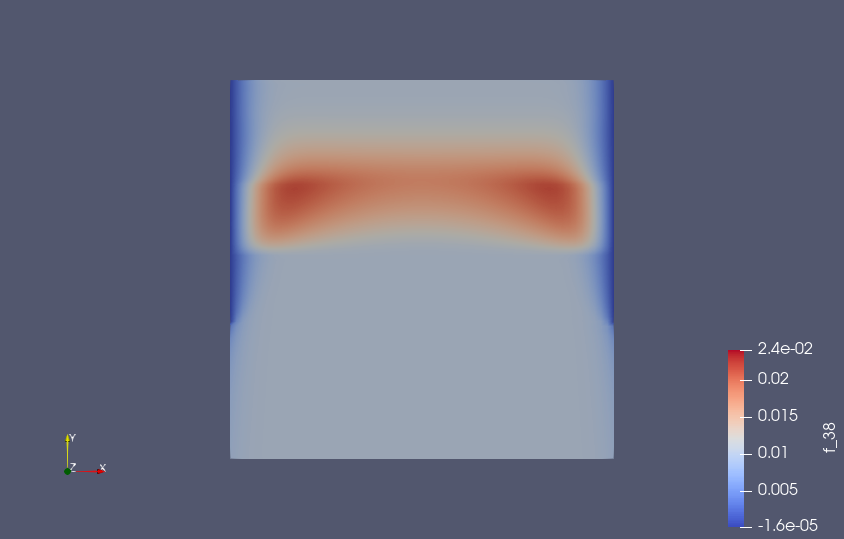
\includegraphics[width=\textwidth]{24rescaledZinc.png}
%     \caption{Re-scaled basic model Zn after 24 hours for comparison}
%     \end{subfigure}
% \end{figure}
% \begin{figure}
%     \centering
%     \caption{Distance and DMA exudation increased}
%     \begin{subfigure}[t]{0.45\textwidth}
%     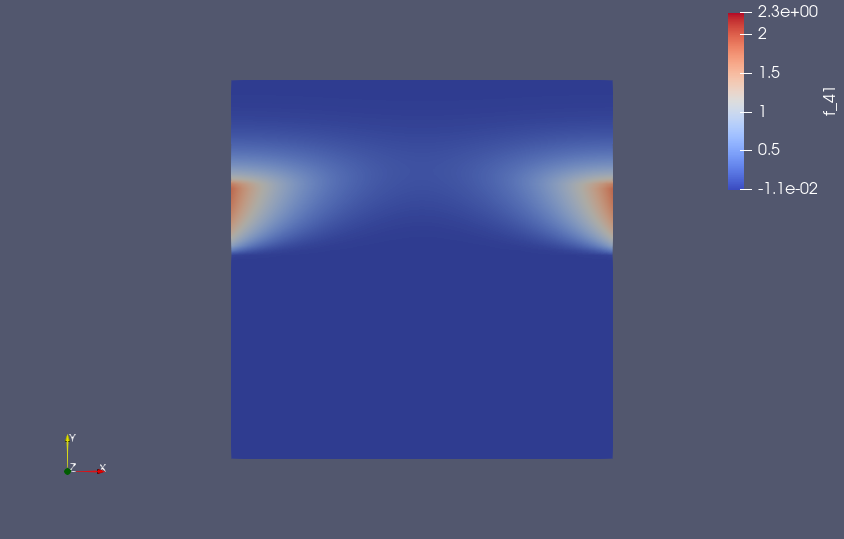
\includegraphics[width=\textwidth]{IncreasedZnAbsorbDMA24.png}
%     \caption{0.08 apart, rate of Zn absorption increased by $0.5e^{-2}$, DMA after 24 hours}
%     \end{subfigure}
%     \begin{subfigure}[t]{0.45\textwidth}
%     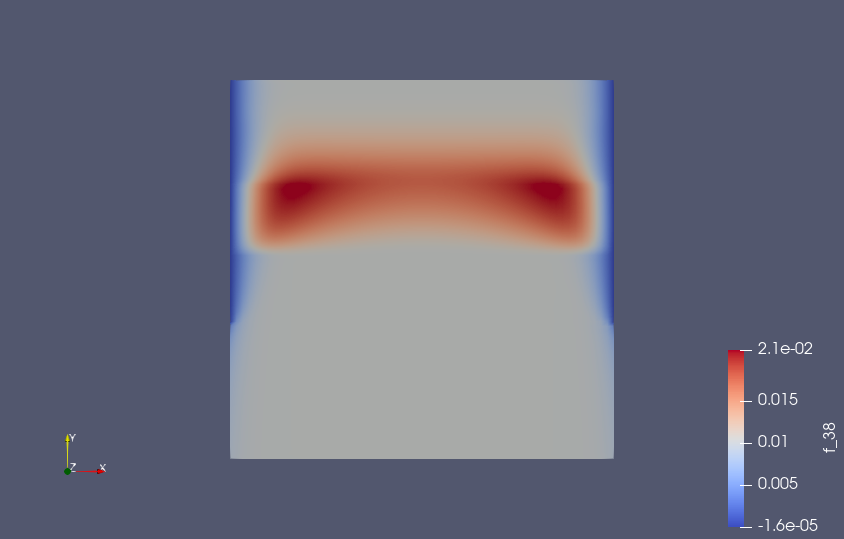
\includegraphics[width=\textwidth]{BasictoComparetoDistanceZn.png}
%     \caption{Re-scaled basic model Zn after 24 hours for comparison}
%     \end{subfigure}
% \end{figure}
% \begin{figure}
%     \centering
%     \begin{subfigure}[t]{0.45\textwidth}
%     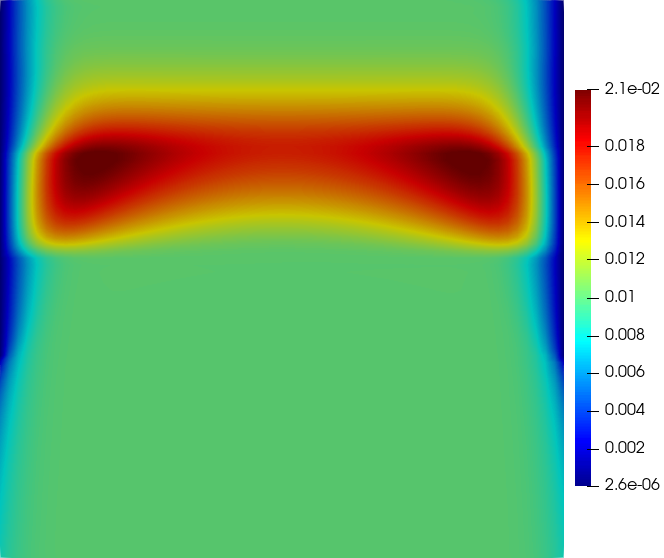
\includegraphics[width=\textwidth]{IncreasedZnAbsorbZn24.png}
%     \caption{0.08 apart, rate of Zn absorption increased by $0.5e^{-2}$, Zn after 24 hours}
%     \end{subfigure}
%     \begin{subfigure}[t]{0.45\textwidth}
%     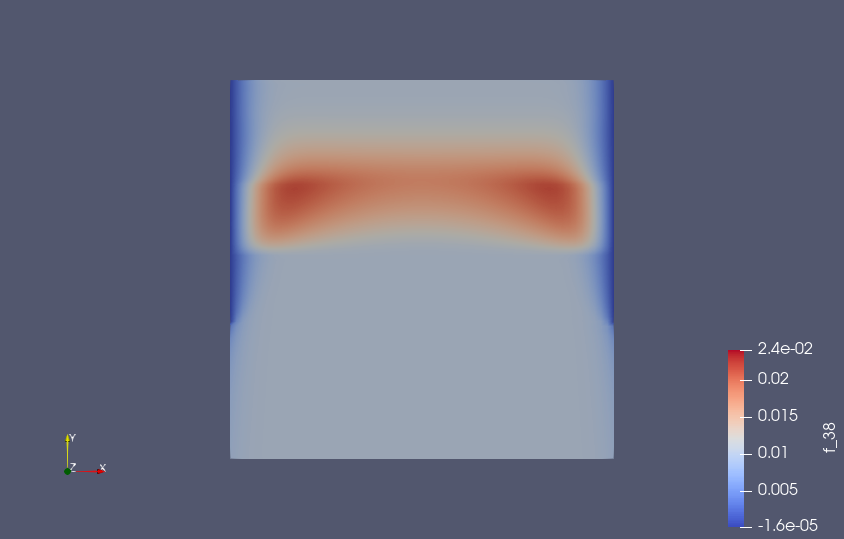
\includegraphics[width=\textwidth]{24rescaledZinc.png}
%     \caption{Re-scaled basic model Zn after 24 hours for comparison}
%     \end{subfigure}
% \end{figure}











%%%%%%%%%%%%%%%%%%%%%%%%%%%%%%%%%%%%%%%%%
%%%%%%%%%%%%%%%%%%%%%%%%%%%%%%%%%%%%%%%%%
%%%%%%%%%%%%%%%%%%%%%%%%%%%%%%%%%%%%%%%%%
\newpage
\section{Existence of Solutions}
\label{sec:Existence}

Taking into account the extensions of the original system from \cite{Ptashnyk-2011}, a more general version of system \eqref{eq:system-Zinc} is studied in this section. 

Here, let \(y(x,t)\) and \(s(x,t)\) be vector functions from \(\Omega \times [0,T]\) in \(\R^{n}\) where for convenience we write \( x = (r,z) \in \Omega\) and also \(\Sigma = \Gamma \times (0,T)\). For each \(\ell \in \llb1,n\rrb\), let us define the uniformly elliptic operator \(L^\ell\) as
\[
	L^\ell y^\ell = \nabla \cdot (a^\ell \nabla y^\ell) + b^\ell \cdot \nabla y^\ell
	= \sum_{i=1}^{2}  \sum_{j=1}^2 \pd{ }{x_i} \big( a_{i,j}^\ell \pd{ }{x_j} y^\ell \big) + \sum_{i=1}^2 b_i^\ell \pd{ }{x_i} y^\ell,
\]
where \(a^\ell\), \(b^\ell \in L^\infty (Q)\), with \(a^\ell\) a diagonal matrix such that \(a_{i,i} \geq 0\) and
\[
	\sum_{i=1}^{2}  \sum_{j=1}^2 a_{i,j}^\ell (x,t) \xi_i \xi_j \geq \theta |\xi|^2,
\]
for some \(\theta > 0\) and all \((x,t) \in Q\), \( \xi \in \R^2\).
%
Moreover, let \(F: \R^n \to \R^n\) such that each component \( F^\ell \) belongs to\( \in C^1 (\R) \cap L^\infty (\R)\), is Lipschitz continuous, and non negative for non negative arguments, and let \(h\in L^2 (\R^n,[0,T]) \) affine on \(y\), and such that \(h(0,t) \leq M \) for all \(t\).
Now, let \(G \in C^\infty(\R^{2n}, \R^n)\) be bilinear such that each \( G^\ell(s,\cdot)\) is linear in \( y\) for fixed \(s\), and each \( G^\ell (\cdot, y)\) depends linearly only on \( s^\ell\) for fixed \(y\). Also, we assume that \(-G\) has the positiveness property that \(-G^\ell (0, y) \geq 0\) if \( y\geq 0\) component-wise. We will present a precise form for \(h\) and \(G\) later.
Finally, let the initial conditions be \( y_0, s_0^\ell \in L^\infty (\Omega)\).

We look after the solution of the system
\begin{subequations}
\label{eq:pde-ode-sys-a}
\begin{align}
	\pd{ }{t} y^\ell &= L^\ell y^\ell - y^\ell F^\ell(y^\ell) + G^\ell(s^\ell,y^1,\ldots y^n) 		&& \text{in } Q, \forall \ell \in \llb 1,n\rrb,
	\\
	\label{sys:coupled-ode}
	\pd{ }{t} s^\ell &= -G^\ell(s^\ell,y^1,\ldots y^n)				&& \text{in } Q,\forall \ell \in \llb 1,n\rrb,
	\\
	 (a^\ell \nabla y^\ell + y^\ell b^\ell) \cdot \vec{n} &= h^\ell (y^\ell, x,t)	&& \text{on } \Sigma,\forall \ell \in \llb 1,n\rrb,
	 \label{eq:1.2.d}
	 \\
	 y^\ell(0) &= y^\ell_{0}			 && \text{in } \Omega, \forall \ell \in \llb 1,n\rrb,
	 \\
	 s^\ell(0) &= s^\ell_{0}			 && \text{in } \Omega, \forall \ell \in \llb 1,n\rrb.
\end{align}
\end{subequations}
Here the set \( \llb 1,n\rrb\) is just the integer interval with extremes \(1\) and \(n\), namely
\[
	\llb 1,n\rrb = \{1,2,\ldots, n-1, n\}.
\]

We are interested in particular for \(G\) to be in the form
\begin{equation}
\label{eq:form_of_G}
	G^\ell (s^\ell,y) = \beta_0^\ell s^\ell - \gamma^\ell y^\ell + \sum_{\substack{1\le i\le n\\ i\neq \ell}} \beta_i^\ell y^i s^\ell,
\end{equation}
where for the positivity assumption we will require \( \gamma^\ell > 0\). We will further assume that \(\beta_i^\ell \geq 0\) for all \(i \in \llb 0,n\rrb \setminus\{\ell\}\). Similarly, each component of \(h\) can be written as
\begin{equation}
\label{eq:form_of_h}
	h^\ell(y^\ell,x,t) = \alpha^\ell (x,t) y^\ell + \nu^\ell (x,t),
\end{equation}
with \(\nu^\ell \) a bounded function, and both \(\alpha^\ell \) and \(\nu^\ell \) integrable. Without loosing generality, let us assume further that \(\alpha^\ell \) and \(\nu^\ell \) are continuous by parts and that \(\alpha^\ell \) is bounded as well. Finally, let us assume that \( \nu^\ell \geq 0\).


%%%%%%%%%%%%%%%%%%%%%%%%%%%%%%%%%%%%%%%%%%%%%%%%%%
%%%%%%%%%%%%%%%%%
\subsection{Analysis of the general coupled system}

In this section we will follow a similar procedure as \cite{Eisenhofer-2013,Ptashnyk-2010,Marciniak-2010}, and \cite{Ptashnyk-2016} to
determine and study a solution of coupled PDE-ODE systems. The scheme is as follows: (a) Show that for fixed \(y\) there is a unique solution of the ODE system. (b) Show that for fixed \(s\) and a linearisation on \(y\) there is a unique solution of the PDE system. (c) Show that the mapping that takes an initial \(y\) and solves the decoupled ODE-PDE system has a fixed point. 
Along this procedure the boundedness of solutions as well as their non negativity will be shown.

Let us begin defining the convex subspace of \((L^2 (Q))^n\):
\[
	Y = \big\{ y \in	(L^2 (Q))^n:\, 	%\big( 0,T, L^\infty(\Omega) \big): \, 
	0 \leq y(x,t) \leq \vartheta \quad\text{for a.e.}\quad (x,t) \in Q \big\}
\]
for a fixed \(\vartheta > 0\).
%
The existence of a solution of \eqref{eq:pde-ode-sys-a} is equivalent to the existence
of a fixed point of \(K\) defined on 
%\(L^2 \big( (0,T), (H^1(\Omega))^n \big) \cap Y \), 
\(Y\),
%
%
%\( L^2 (0,T,Z)\) with \(Z = \big( (H^1(\Omega))^n \times (L^2(\Omega))^n \big) \cap \big(L^\infty(\Omega)\big)^{2n}\) and its derivative in \(L^2 (0,T, Z^*) \). 
%\( L^2 (0,T,Y)\), with \(Y = \big(H^1(\Omega) \cap L^\infty(\Omega)\big)^{n}\) 
%
%
and its derivative in \(L^2 ( 0,T;(H^1(\Omega))^{*n} )\),
by \( y_m = K(y_{m-1}) \), where \(y_m\) is a solution of the system
\begin{subequations}
\label{sys:de-coupled}
\begin{align}
	\pd{ }{t} y_m^\ell &= L^\ell y_m^\ell - y^\ell_m F^\ell(y_{m-1}^\ell) + G^\ell(s_m^\ell,y_{m}^1,\ldots y_{m}^n) 		&& \text{in } Q, \forall \ell \in \llb 1,n\rrb,
	\label{sys:de-coupled-pde}
	\\
	\pd{ }{t} s_m^\ell &= -G^\ell(s_m^\ell,y_{m-1}^1,\ldots y_{m-1}^n)				&& \text{in } Q,\forall \ell \in \llb 1,n\rrb,
	\label{sys:de-coupled-ode}
	\\
	 (a^\ell  \nabla y_m^\ell + y_m^\ell b^\ell) \cdot \vec{n} &= h^\ell (y_{m}^\ell, x,t)	&& \text{on } \Sigma,\forall \ell \in \llb 1,n\rrb,
	 \label{sys:de-coupled-pde-b}
	 \\
	 y_m^\ell(0) &= y^\ell_{0}			 && \text{in } \Omega, \forall \ell \in \llb 1,n\rrb,
	 \label{sys:de-coupled-pde-i}
	 \\
	 s_m^\ell(0) &= s^\ell_{0}			 && \text{in } \Omega, \forall \ell \in \llb 1,n\rrb.
	 \label{sys:de-coupled-ode-i}
\end{align}
\end{subequations}

Now we can divide the system in two parts. First, the analysis of the differential equations \eqref{sys:de-coupled-ode}, and then the analysis for the partial differential equations in \eqref{sys:de-coupled-pde}.

%%%%%%%%%%%%%%%
%%%%%%%%%%%%%%%
\vspace{1\baselineskip}
\noindent\emph{(A) Subsystem of ordinary differential equations}
\vspace{0.5\baselineskip}

Observe that for any given \(y_{m-1} \in Y \), then the ODE system \eqref{sys:de-coupled-ode}--\eqref{sys:de-coupled-ode-i} is a non-homogeneous linear system of ordinary differential equations.
%
Carathéodory's theorem gives us that there exists a unique solution \(s_m \in H^{1} ( 0,T;(L^2(\Omega))^{n}  )\) for some \(T\).
	%
	We can improve this regularity. Recalling \eqref{eq:form_of_G}, for any \(y_{m-1} \in \R^n\), \(-G(s_m,y_{m-1})\) can be written as
	\[
		-G(s_m,y_{m-1}) = B(y_{m-1})s_m + C(y_{m-1})
	\]
	with \(C\) a vector and \(B\) a diagonal matrix. As \(B(y)(t_1)\) commutes with \( B(y)(t_2)\), for any \(t_1, t_2 \in \R\) (as it is a diagonal matrix), we further have that there is a global \(H^1 (0,T;(L^2(\Omega))^n )\) solution given by
	\[
		s_m(t) = e^{\overline{B}(t)} s_0 + \int\limits_0^t e^{\overline{B}(t)- \overline{B}(r)} C(y_{m-1}) \dif r
	\]
	with \( \overline{B}(t) = \int_0^t B(y_{m-1})(\xi) \dif \xi\) \cite{Schaeffer-2016}. 
	%
	Particularly, each row of \(s_m\) will be given exactly by
	\begin{equation}
	\label{eq:solution_of_ode}
		s_m^\ell (t) = s_0 \, e^{ \int_0^t B_{\ell,\ell} (y_{m-1})(\xi) \dif \xi } + \int\limits_0^t 
		e^{ \int_0^t B_{\ell,\ell} (y_{m-1})(\xi) \dif \xi - \int_0^r  B_{\ell,\ell} (y_{m-1})(\xi) \dif \xi} 
		C^{\ell} (y_{m-1})(r) \dif r.
	\end{equation}
	Here we have that
	\[
		B_{\ell,\ell} = -\beta_0^\ell - \sum_{\substack{1\le i\le n\\ i\neq \ell}} \beta_i^\ell y_{m-1}^i 
		\qquad\text{and}\qquad
		C^\ell (y_{m-1}) = \gamma^\ell y_{m-1}^\ell,
	\]
	where we have to recall that \( \gamma_i^\ell \geq 0\) and \( y_{m-1}^i \in Y\). As a result, \eqref{eq:solution_of_ode} yields an always non negative solution \( s_m \in L^\infty (Q)\).
	If we did not have a closed expression for \(s_m\), we could have argued via the work of \cite{Horvath-1998} on positiveness for ODE systems, which requires the positiveness assumption for \(-G\) and \(s_0\). In any case, we have got that \( s_m^\ell \in H^1(0,T;L^2(\Omega) ) \cap L^\infty (Q)\) and \(s_m^\ell \geq 0\) for each \(\ell\in \llb 1,n\rrb\).



%%%%%%%%%%%%%%%
%%%%%%%%%%%%%%%
\vspace{1\baselineskip}
\noindent\emph{(B) Subsystem of partial differential equations}
\vspace{0.5\baselineskip}


Next we turn to the linear system \eqref{sys:de-coupled-pde}, \eqref{sys:de-coupled-pde-b}, \eqref{sys:de-coupled-pde-i} of parabolic differential equations. Further, as we already have \(s_m\), it is now \emph{decoupled} from the ODE system. Following \cite{Evans-2010}, we consider a different viewpoint by associating with \(u\) a mapping \( \mathbf{u} : [0,T] \to V\), such that \( \mathbf{u}(t)(x) = u(x,t)\), with \(V\) an appropriate Banach space. 

We say that a vector function \(y_m\) is a weak solution of \eqref{sys:de-coupled-pde} with boundary conditions \eqref{sys:de-coupled-pde-b} and initial conditions \eqref{sys:de-coupled-pde-i} if each \(y^\ell_m \in L^2(0,T;H^1(\Omega)) \) and \( \pd{y_m^\ell}{t} \in L^2(0,T;(H^1(\Omega))^*) \)  satisfy
	\begin{align}
		\int\limits_0^T \int\limits_\Omega \pd{\by_m^\ell}{t} v  \dif x \dif t
		&=
		\int\limits_0^T 
		\big( h^\ell (\by_m^\ell,x,t), v\big)_{L^2 (\Gamma)} -  \big( a^\ell \nabla \by_m^\ell + \by_m^\ell b^\ell , \nabla v\big)_{L^2(\Omega)}  \dif t
		\notag
		\\
		&\qquad\qquad\,\,\,
		+
		\int\limits_0^T \big(-\by_m^\ell F^\ell(\by_{m-1}^\ell) + G^\ell(\mathbf{s}_m^\ell,\mathbf{y}_{m}), v \big)_{L^2(\Omega)} \dif t
		\notag
		\\
		\label{eq:linear-parabolic}
		&=
		-
		\int\limits_0^T 
		\int\limits_\Omega (a^\ell \nabla y_m^\ell + y_m^\ell b^\ell ) \cdot \nabla v \dif x \dif t
		+
		\int\limits_0^T 
		\int\limits_\Gamma h^\ell (y_{m}^\ell,x,t) v \dif \sigma\dif t 
		\\ &\qquad\qquad\qquad	\notag
		+
		\int\limits_0^T \int\limits_\Omega 
		-y_m^\ell F^\ell(y^\ell_{m-1}) v + G^\ell(s_m^\ell, y_{m-1}) v \dif x \dif t
	\end{align}
	for all \( v \in L^2 (0,T;H^1(\Omega) ) \), and with the initial condition \( y_m^\ell \to y_0^\ell \) in \(L^2(\Omega)\) as \( t\to 0\), for all \(\ell \in \llb 1,n\rrb\). 
	
Problem \eqref{eq:linear-parabolic} has been extensively studied in the literature, see for example \cite{Ladyzenskaja-1968} or \cite{Pao-1993}. Using Galerkin's method, we can prove that there is a unique solution given component-wise as the element \(y_m^\ell \in L^2(0,T;\)  \( H^1(\Omega)) \cap L^\infty(0,T; L^2(\Omega))\) with \( \pd{y_m^\ell}{t} \in L^2(0,T; (H^1(\Omega))^*) \).



%%%%%%%%%%%%%%%
%%%%%%%%%%%%%%%
%%%%%%%%%%%%%%%
%\subsubsection{Proof of existence of \(y_m\)}
\vspace{1\baselineskip}
\noindent\textbf{Proof of existence of \(y_m\)}
\vspace{0.5\baselineskip}
	
	We will adapt ideas from \cite{Ladyzenskaja-1968,Troltzsch-2010} and \cite{Evans-2010}.
	
	Consider a fundamental system of functions \((w_k)_{k\in \N^*}\) in \(H^1(\Omega)\); i.e., they form an orthogonal basis in \(H^1(\Omega)\), and for simplicity let us assume further that they are orthonormalised in \(L^2(\Omega)\). Moreover, let us define\footnote{Notice that \(a^\ell\) is linear in \( y_m\), not only in \(y_m^\ell\).}
	\[
		a^\ell [\by_m,v;t] := 
		\int\limits_\Omega (a^\ell \nabla y_m^\ell + y_m^\ell b^\ell ) \cdot \nabla v \dif x + \int\limits_\Omega d^\ell (y_m) v \dif x
		- \int\limits_\Gamma \alpha^\ell (x,t) y_m^\ell v \dif \sigma
	\]
	where we have used the explicit form of \(h^\ell\) presented in \eqref{eq:form_of_h}, and \(d^\ell\) is given by
	\[
		d^\ell (y_m) := y_m^\ell F^\ell(y_{m-1}^\ell) + \gamma^\ell y_m^\ell - s_m^\ell \sum_{\substack{1\le i\le n\\ i\neq \ell}} \beta_i^\ell y_m^i.
	\]
	Also let us define the two linear functionals in \(v\)
	\[
		\mathbf{f}^\ell (t) := \beta_0^\ell \int\limits_\Omega s_m^\ell  v \dif x
		\qquad\text{and}\qquad
		\mathbf{g}^\ell (t) :=  \int\limits_\Gamma \nu^\ell (x,t)  v \dif \sigma.
	\]
	Notice that these are well defined as \(F^\ell\) and \(s_m^\ell\) are bounded.
	
	
	
	
	
	Fix a positive integer \(N\). We will seek for an approximate solution in the form
	\begin{equation}
	\label{eq:ansatz}
		\mathbf{y}_m^{\ell,N} (t)(x) = \sum_{k=1}^N c_k^{\ell,N} (t) w_k(x)
	\end{equation}
	so that the coefficients \( c_k^{\ell,N} \) are determined by the conditions 
	\begin{equation}
	\label{sys-pde-pre-galerkin}
		\big(\pd{ }{t} \by_m^{\ell,N}, w_k\big)_\Omega + 
		a^\ell [\mathbf y_m^{N}, w_k; t] 
		=
		\big( \mathbf{f}^\ell (t), w_k \big)_{\Omega} + \big(\mathbf{g}^\ell (t),  w_k \big)_{\Gamma}
	\end{equation}
	for almost every \(t\in (0,T)\) with the initial condition \( c_k^N (0) =  (\by^\ell (0), w_k)_\Omega = (y_0^\ell, w_k)_\Omega\)  for all \(k \in \llb 1,N\rrb\). 
	
	Substituting the \emph{ansatz}  \eqref{eq:ansatz} in \eqref{sys-pde-pre-galerkin} and making use of the orthonormality, we see that
	\begin{align*}
		a^\ell [\mathbf y_m^{N}, w_k; t] 
		&= 
		\sum_{i=1}^N  \bigg[ c_i^{\ell,N}  \int\limits_\Omega  ( a^\ell \nabla w_i + w_i b^\ell) \cdot \nabla w_k \dif x -  c_i^{\ell, N} \int\limits_\Gamma \alpha^\ell w_i w_k \dif \sigma
		\\
		&\qquad
		+ \int\limits_\Omega 
		c_i^{\ell,N} (w_i F^\ell w_k) + \frac{1}{N}  \gamma^\ell c_k^{\ell,N} -  \sum_{\substack{1\le j\le n\\ j\neq \ell}} \beta_j^\ell c_i^{j,N} (s_{m}^\ell w_i w_k)
		 \dif x
		\bigg] =: A^\ell (c^{N})
	\end{align*}
	As a result, we get the system
	\begin{subequations}
	\label{sys-pde-galerkin}
	\begin{align}
		\pd{ }{t} c_k^{\ell,N} + A^\ell (c^{N}) &= l_k^\ell (t)		\\
		c_k^{\ell,N} (0) &= (y_0^\ell, w_k)
	\end{align}
	\end{subequations}
	for almost every \(t\in (0,T)\), all \( k\in \llb1,N\rrb\), and \(n\in \llb 1,n\rrb\); with the functions \( l^\ell_k(t) = \big( \mathbf{f}^\ell (t), w_k \big)_{\Omega} + \big(\mathbf{g}^\ell (t),  w_k \big)_{\Gamma}\).
	
	The system \eqref{sys-pde-galerkin} is a linear system of ordinary differential equations in terms of \(c_k^{\ell,N}\) with initial value conditions. Owing to Carathèodory's theorem, there exists a unique absolutely continuous solution \( c^N \in \big(H^1(0,T)\big)^{nN}\). Now, if we put \(c^{\ell,N}\) as a test function in \eqref{sys-pde-pre-galerkin} and sum over \(k\), we get that
	\begin{equation}
	\label{eq:result-galerkin}
		\big(\pd{ }{t} \by_m^{\ell,N}, \by_m^{\ell,N}\big)_\Omega + 
		a^\ell [\mathbf y_m^{N}, \by_m^{\ell,N}; t] 
		=
		\big( \mathbf{f}^\ell (t), \by_m^{\ell,N} \big)_{\Omega} + \big(\mathbf{g}^\ell (t),  \by_m^{\ell,N} \big)_{\Gamma}
	\end{equation}
	for almost every \(t\in (0,T)\) and all \(\ell \in \llb 1,n\rrb\). 
	
	 Now, for an arbitrary but fixed \(\tau \in (0,T]\) and any \(\ell \in \llb 1,n\rrb\), we have the identity 
	 \[
	 	\int\limits_0^\tau \big(\pd{ }{t} \by_m^{\ell,N}(t), \by_m^{\ell,N} (t) \big)_\Omega \dif t
		=
		\frac{1}{2} \int\limits_0^\tau  \pd{ }{t} \| \by_m^{\ell,N}(t) \|_\Omega^2 \dif t
		=
		\frac{1}{2} \| \by_m^{\ell,N}(\tau) \|_\Omega^2 - \frac{1}{2} \| \by_m^{\ell,N}(0) \|_\Omega^2.
	 \]
	 If we integrate \eqref{eq:result-galerkin} over \([0,\tau]\) and incorporate this last identity, we get that for any \(\ell \in \llb 1,n\rrb\) it holds
	 \begin{align}
	 \label{eq:estimate-integrationbyparts}
	 	\frac{1}{2} \| \by_m^{\ell,N}(\tau) \|_\Omega^2
		+ 
		\int\limits_0^\tau a^\ell [\mathbf y_m^{N}, \by_m^{\ell,N}; t] \dif t
		=
		\frac{1}{2} \| \by_m^{\ell,N}(0) \|_\Omega^2 + 
		\int\limits_0^\tau \big( \mathbf{f}(t), \by_m^{\ell,N} (t) \big)_{\Omega} + \big(\mathbf{g}(t),  \by_m^{\ell,N} (t) \big)_\Gamma \dif t.
	 \end{align}
	Additionally, by Bessel's inequality, we have that
	\begin{equation}
	\label{eq:estimate-i}
		\| \by_m^{\ell,N}(0) \|_\Omega^2 = \sum_{k=1}^N |c_k^{\ell,N}(0)|^2 = \sum_{k=1}^N | (y_0^\ell, w_k) |^2 \leq \|y_0^\ell\|_\Omega^2.
	\end{equation}
	
	
	
	Moreover, it is not hard to show, using Cauchy's inequality, that for any element \(v\in (H^1(\Omega))^n\) the inequality
	\[
		\frac{1}{2} \theta \|\nabla v^\ell \|^2_{\Omega}
		\leq a^\ell [v,v^\ell;t]  + \frac{1}{2} c_{s,b,\alpha,F}^\ell \sum_{k=1}^n \|v^k\|^2_{\Omega} 
	\]
	is satisfied, where \(c_{s,b,\alpha,F}^\ell\) is a constant depending linearly on the supremum norms of \(s_m^\ell, b^\ell, \alpha^\ell\), and \(F^\ell(y_{m-1}^\ell)\). Furthermore, applying Cauchy's inequality again we get
	\[
		\big| \big( \mathbf{f}^\ell , \by_m^{\ell,N} \big)_{\Omega} \big| \leq \frac{1}{2} \|\mathbf{f}^\ell \|^2_{\Omega} + \frac{1}{2} \|\by_m^{\ell,N}\|_{\Omega}^2
		\qquad\text{and}\qquad
		\big(\mathbf{g}^\ell ,  \by_m^{\ell,N} \big)_\Gamma
		\leq \varepsilon \|\mathbf{g}^\ell \|^2_{\Gamma} + \frac{1}{4\varepsilon} \|\by_m^{\ell,N}\|_{\Gamma}^2.
	\]
	This way we can use a proper selection of \(\varepsilon\) alongside the trace inequality to obtain, for some \(C_1\) and \(C_2\), that
	\[
		\pd{ }{t} \| \by_m^{\ell,N} \|^2_\Omega + \theta \|\nabla \by_m^{\ell,N}\|^2_{\Omega}
		\leq C_1 \sum_{k=1}^n \|\by_m^{k,N}\|^2_{\Omega} + C_2\big(\|\mathbf{f}^\ell \|^2_{\Omega} + \|\mathbf{g}^\ell \|^2_{\Gamma} \big).
	\]
	\begin{comment}
	Adding the norm of \(\by_m^{\ell,N}\) at both sides of the inequality, we get
	\[
		\pd{ }{t} \| \by_m^{\ell,N} \|^2_\Omega + \theta \| \by_m^{\ell,N}\|^2_{H^1(\Omega)}
		\leq C_1 \sum_{k=1}^n \|\by_m^{k,N}\|^2_{H^1(\Omega)} + C_2\big(\|\mathbf{f}^\ell\|^2_{\Omega} + \|\mathbf{g}^\ell\|^2_{\Gamma} \big),
	\]
	with an updated \(C_1\). 
	\end{comment}
	We can sum the inequalities with respect to \(\ell\) to obtain
	\begin{equation}
	\label{eq:estimate-differential}
		\pd{ }{t} \sum_{\ell=1}^n \| \by_m^{\ell,N} \|^2_\Omega + \theta \sum_{\ell=1}^n \| \nabla \by_m^{\ell,N}\|^2_{\Omega}
		\leq C_1 \sum_{\ell=1}^n \|\by_m^{\ell,N}\|^2_{\Omega} + C_2 \sum_{\ell=1}^n \big(\|\mathbf{f}^\ell\|^2_{\Omega} + \|\mathbf{g}^\ell\|^2_{\Gamma} \big),
	\end{equation}
	with updated \(C_1\) and \(C_2\).
	%
	Notice that this is a differential inequality, so we can use Grönwall's inequality to get the estimate
	\begin{equation}
	\label{eq:Grownwall}
		\sum_{\ell=1}^n \| \by_m^{\ell,N} (t) \|^2_\Omega \leq \sum_{\ell=1}^n  e^{C_1 t} \bigg(  \| \by_m^{\ell,N} (0) \|^2_\Omega
			+ C_2 \int\limits_0^t \|\mathbf{f}^\ell (r)\|^2_{\Omega} + \|\mathbf{g}^\ell (r)\|^2_{\Gamma} \dif r
		\bigg).
	\end{equation}
	Now, by \eqref{eq:estimate-i} and the fact that \eqref{eq:Grownwall} is a sum of positive terms, we get the particular estimate
	\begin{equation}
	\label{eq:estimate-maxnorm}
		\max_{0\leq t \leq T} \| \by_m^{\ell,N} (t) \|^2_\Omega \leq C \sum_{k=1}^n  \bigg(  \| \by_0^k \|^2_\Omega
			+ \|\mathbf{f}^k\|^2_{L^2(0,T;L^2(\Omega))} + \|\mathbf{g}^k\|^2_{L^2(0,T;L^2(\Gamma))}
		\bigg)
	\end{equation}
	for each \(\ell \in \llb 1,n\rrb\).
	
	Now we can use \eqref{eq:estimate-integrationbyparts} replacing \(\tau\) with \(T\), estimate \eqref{eq:estimate-differential} completing the \(H^1\)--norm of each \(y_m^{\ell,N}\), and estimate \eqref{eq:estimate-maxnorm} to get
	\[
		\|\by_m^{\ell,N} \|^2_{L^2(0,T, H^1(\Omega))}
		\leq 
		C \sum_{k=1}^n \bigg(  \| \by_0^k \|^2_\Omega + \|\mathbf{f}^k\|^2_{L^2(0,T, L^2(\Omega))} + \|\mathbf{g}^k\|^2_{L^2(0,T, L^2(\Gamma))} \bigg),
	\]
	where \(C\) is a generic positive constant. With these estimates we have got that
	\[
		\| \by_m^{\ell,N} \|^2_{L^\infty (0,T;L^2(\Omega) )} 
		+ \|\by_m^{\ell,N} \|^2_{L^2(0,T;H^1(\Omega))}
		\leq 
		C \sum_{k=1}^n \bigg(  \| \by_0^k \|^2_\Omega + \|\mathbf{f}^k\|^2_{L^2(0,T;L^2(\Omega))} + \|\mathbf{g}^k\|^2_{L^2(0,T;L^2(\Gamma))} \bigg);
	\]
	%or alternatively, that the \(V_2(Q)\) norm of \(\by_m^{\ell,N}\) is bounded by a constant independent of \(N\) and \(\ell\), let us call it \(K_{m}\). 
	where the term on the right is a constant independent of \(N\), let us call it \(K_{m}\). 
	Observe that in particular \eqref{eq:estimate-maxnorm} yields \( \|\by_m^{\ell,N}(t)\|_{\Omega}^2 \leq K_{m} \) and in view of the orthonormality
	\begin{equation}
	\label{eq:boundness-of-coeffs}
		\sum_{k=1}^N |c_k^N(t)|^2 \leq K_{m}
	\end{equation}
	for all \(t\in [0,T]\) and \( N \in \N^*\).
	
	We can even go a step further. Fix any \(v\in H^1(\Omega)\) with \(\|v\|_{H^1(\Omega)} \leq 1\) and write it as \( v = v^1 + v^2\), where \(v^1\) is generated by the span of \( \{w_k\}_{k=1}^N\) and \( (v^2,w_k) = 0\) for all \( k \in \{1,\ldots,N\}\). Since the functions \( (w_k)_{k\in \N^*}\) are orthogonal in \(H^1(\Omega)\), we get \( \|v^1\|_{H^1(\Omega)} \leq \|v\|_{H^1(\Omega)} \leq 1 \). Utilising \eqref{sys-pde-pre-galerkin}, we get that for almost every \(t\in (0,T)\)
	\[
		\big(\pd{ }{t} \by_m^{\ell,N}, v^1\big)_\Omega + 
		a^\ell [\mathbf y_m^{N}, v^1; t] 
		=
		\big( \mathbf{f}^\ell (t), v^1 \big)_{\Omega} + \big(\mathbf{g}^\ell (t),  v^1 \big)_{\Gamma}.
	\]
	Then \eqref{eq:ansatz} implies
	\[
		\big\langle \pd{ }{t} \by_m^{\ell,N}, v \big\rangle =
		\big(\pd{ }{t} \by_m^{\ell,N}, v\big)_\Omega =
		\big(\pd{ }{t} \by_m^{\ell,N}, v^1\big)_\Omega 
		=
		\big( \mathbf{f}^\ell (t), v^1 \big)_{\Omega} + \big(\mathbf{g}^\ell (t),  v^1 \big)_{\Gamma}
		- a^\ell [\mathbf y_m^{N}, v^1; t] .
	\]
	Continuity of \(a^\ell\) and the norm of \(v\) with by Cauchy--Bunyakovsky--Schwarz inequality give
	\[
		\Big| \big\langle \pd{ }{t} \by_m^{\ell,N}, v \big\rangle \Big|
		\leq C \sum_{k=1}^n
		\big( \|\mathbf{f}^k\|_{\Omega} + \|\mathbf{g}^k\|_{\Gamma} + \|\by_m^{k,N}\|_{H^1(\Omega)} \big);
	\]
	thus the operator norm of \(\pd{ }{t} \by_m^{\ell,N}\) is bounded for almost everywhere \(t\in (0,T)\). Additionally, we can square the last inequality, use again Cauchy's inequality and get
	\[
		\big\| \pd{ }{t} \by_m^{\ell,N} \big\|_{H^1(\Omega)^*} 
		\leq C \sum_{k=1}^n \big( \|\mathbf{f}^k\|_{\Omega} + \|\mathbf{g}^k\|_{\Gamma} + \|\by_m^{k,N}\|_{H^1(\Omega)} \big) ;
	\]
	and therefore
	\begin{align*}
		\int\limits_0^T \big\| \pd{ }{t} \by_m^{\ell,N} \big\|^2_{H^1(\Omega)^*} \dif t 
		\leq C\sum_{k=1}^n \bigg(  \| \by_0^k \|^2_\Omega + \|\mathbf{f}^k\|^2_{L^2(0,T, L^2(\Omega))} + \|\mathbf{g}^k\|^2_{L^2(0,T, L^2(\Gamma))} \bigg).
	\end{align*}
	As a result, we have got
	\begin{equation}
	\label{eq:energy-estimates}
	\begin{aligned}
		\| \by_m^{\ell,N} \|^2_{C([0,T];L^2(\Omega) )} 
		&+ \|\by_m^{\ell,N} \|^2_{L^2(0,T; H^1(\Omega))}
		+  \| \partial_t \by_m^{\ell,N} \|^2_{L^2(0,T;H^1(\Omega)^*)}
		\\
		&\qquad\qquad\leq 
		C \sum_{k=1}^n \bigg(  \| \by_0^k \|^2_\Omega + \|\mathbf{f}^k\|^2_{L^2(0,T;L^2(\Omega))} + \|\mathbf{g}^k\|^2_{L^2(0,T;L^2(\Gamma))} \bigg).
	\end{aligned}
	\end{equation}
	
	%
	% Made it!
	%
	According to the energy estimates \eqref{eq:energy-estimates} and \eqref{eq:boundness-of-coeffs}, we see that \((\by_m^{\ell,N})_{N\in \N^*}\) is bounded in \(L^2(0,T;H^1(\Omega))\), \((\partial_t \by_m^{\ell,N})_{N\in \N^*}\) is bounded in \(L^2(0,T;H^1(\Omega)^*)\), and all \( c_k^{\ell,N} (t)\) are essentially bounded for all \(\ell\), \(k\), \(N\), and \(t\). 
	
	
	According to the energy estimates \eqref{eq:energy-estimates}, we see that the sequence \((\by_m^{\ell,N_q})_{N_q\in \N}\)  is bounded in \(L^2(0,T;H^1(\Omega))\) and \((\pd{ }{t}\by_m^{\ell,N_q})_{N_q\in \N}\)  is bounded in \(L^2(0,T;(H^1(\Omega))^*)\). Consequently, there exists a subsequence \((\by_m^{\ell,N_q})_{N_q\in \N}\) and functions \(\by_m^{\ell} \in L^2(0,T;H^1(\Omega))\),  with \(\pd{ }{t}\by_m^{\ell} \in L^2(0,T;(H^1(\Omega))^*)\) for each \(\ell \in \llb1,n\rrb\), such that
	\begin{equation}
	\label{weak-conv}
		\begin{cases}
			\by_m^{\ell,N_q} \rightharpoonup \by_m^{\ell} & \text{weakly in } L^2(0,T;H^1(\Omega)),
			\\
			\pd{ }{t}\by_m^{\ell,N_q} \rightharpoonup \pd{ }{t} \by_m^{\ell} & \text{weakly in } L^2(0,T;H^1(\Omega)^*).
		\end{cases}
	\end{equation}
	Moreover, owing to the weak lower sequential semicontinuity of the norm, we also get that \(\|\by_m^\ell(t)\|_\Omega\) is also bounded by \(K_{m}\), thus \(\by_m^\ell \in L^\infty (0,T; L^2 (\Omega))\).



Now, for a fixed integer \(\tilde n\), let us pick a function \( \bv \in C^1([0,T]; H^1(\Omega))\) of the form
	\begin{equation}
	\label{eq:test-fun-bochner}
		\bv(t) = \sum_{k=1}^{\tilde n} d_k(t) w_k,
	\end{equation}
	with \(\{d_k\}_{k=1}^{\tilde n}\) a set of given functions.
	Let us pick \(N \geq \tilde n\), multiply \eqref{sys-pde-pre-galerkin} by \(c_k\), sum over \(k\) and then integrate with respect to \(t\) to find
	\[
		\int\limits_0^T
		\big\langle \pd{ }{t} \by_m^{\ell,N}, \bv \big\rangle + 
		a^\ell [\mathbf y_m^{N}, \bv; t] \dif t
		=
		\int\limits_0^T
		\big( \mathbf{f}^\ell (t), \bv \big)_{\Omega} + \big(\mathbf{g}^\ell (t),  \bv \big)_{\Gamma}
		\dif t.
	\]
	Using the subsequence and recalling \eqref{weak-conv}, we get
	\begin{equation}
	\label{eq:variational}
		\int\limits_0^T
		\big\langle \pd{ }{t} \by_m^{\ell}, \bv \big\rangle + 
		a^\ell [\mathbf y_m^{\ell}, \bv; t] \dif t
		=
		\int\limits_0^T
		\big( \mathbf{f}^\ell (t), \bv \big)_{\Omega} + \big(\mathbf{g}^\ell (t),  \bv \big)_{\Gamma}
		\dif t.
	\end{equation}
	This equality then holds for all functions \( \bv \in L^2(0,T;H^1(\Omega))\), as functions of the form \eqref{eq:test-fun-bochner} are dense in this space. %In particular, it holds for any \( v \in H^1(\Omega)\) as well. 
	
	To prove that \( \by_m^\ell (0) = y_0^\ell\) it suffices to see that \eqref{eq:variational} can be integrated by parts for all \( \bv \in C^1(0,T;H^1(\Omega))\) with \(\bv(T) = 0\). Again passing through a subsequence, noticing that \( \by_m^{\ell, N_k} (0) \to y_0^\ell\) in \(L^2(\Omega)\), and that \(\bv(0)\) is arbitrary, then we obtain the desired property.
	
	As discussed in \cite{Evans-2010}, uniqueness follows from showing that if \( \by_m^\ell\) and \( \mathbf{u}\) are two solutions of the parabolic problem, then their difference \(\bv^\ell\) satisfies
	\[
		\frac{1}{2}
		\pd{ }{t} \| \bv^\ell \|^2_{\Omega} + 
		a^\ell [\bv, \bv^\ell; t]
		=
		0.
	\]
	The lower bounds of \(a^\ell\) and Gronwall's inequality later imply that \( \bv \equiv 0\).
















%%%%%%%%%%%%%%%
%%%%%%%%%%%%%%%
\vspace{1\baselineskip}
\noindent\emph{(C) Notes on the regularity of \(y_m^\ell\)}
\vspace{0.5\baselineskip}


It is shown in \cite{Evans-2010}, that as \(y_m^\ell \in L^2(0,T; H^1(\Omega)) \) and \(\pd{ }{t} y_m^\ell \in L^2(0,T; (H^1(\Omega))^*) \), then we also have  \(y_m^\ell \in C([0,T]; L^2 (\Omega))\). This way, the follow estimate holds:
	%
	%
	\begin{equation}
	\begin{aligned}
		\| \by_m^{\ell} \|_{C([0,T];L^2(\Omega) )} 
		&+ \|\by_m^{\ell} \|_{L^2(0,T; H^1(\Omega))}
		+  \| \partial_t \by_m^{\ell} \|_{L^2(0,T;H^1(\Omega)^*)}
		\\
		&\qquad\qquad\leq 
		C\sum_{k=1}^n \bigg(  \| \by_0^k \|_\Omega + \|\mathbf{f}^k\|_{L^2(0,T;L^2(\Omega))} + \|\mathbf{g}^k\|_{L^2(0,T; L^2(\Gamma))} \bigg),
	\end{aligned}
	\end{equation}
	for every \( \ell \in \llb 1, n\rrb\).



Now we will proceed to show that the solutions \(y_m\) are uniformly bounded independently.  To do this, we will be using the framework of invariant rectangles \cite{Redlinger-1989,Weinberger-1975}. As pointed out in \cite{Ptashnyk-2016}, the theory of bounded invariant rectangles can be applied to problems of the type \eqref{sys:de-coupled} using a regularisation argument. 

Let us recall here the linear system of partial differential equations given by \eqref{sys:de-coupled-pde}, \eqref{sys:de-coupled-pde-b}, and \eqref{sys:de-coupled-pde-i}, which we include here for clarity:
\begin{subequations}
\label{sys:de-coupled.recalled}
\begin{align}
	\pd{ }{t} y_m^\ell &= L^\ell y_m^\ell - y^\ell_m F^\ell(y_{m-1}^\ell) + G^\ell(s_m^\ell,y_{m}^1,\ldots y_{m}^n) 		&& \text{in } Q, \forall \ell \in \llb 1,n\rrb,
	\label{sys:de-coupled-pde.recalled}
	\\
	 (a^\ell  \nabla y_m^\ell + y_m^\ell b^\ell) \cdot \vec{n} &= h^\ell (y_{m}^\ell,x, t)	&& \text{on } \Sigma,\forall \ell \in \llb 1,n\rrb,
	 \label{sys:de-coupled-pde-b.recalled}
	 \\
	 y_m^\ell(0) &= y^\ell_{0}			 && \text{in } \Omega, \forall \ell \in \llb 1,n\rrb.
	 \label{sys:de-coupled-pde-i.recalled}
\end{align}
\end{subequations}

Now let us introduce the set 
\[
	\Sigma  = \big\{ y \in \R^n :\, 0 \leq y \leq \vartheta  \big\}.
\]
We claim that \(\Sigma\) is an invariant set. 
Let us define \(H(y,t)\) as the reaction term of system \eqref{sys:de-coupled.recalled}; i.e., \( H^\ell (y) := - y^\ell F^\ell(y_{m-1}^\ell) + G^\ell(s_m^\ell, y^1,\ldots y^n) \). Using the explicit formulae for \(G\), we get
\[
	H^\ell (y) = -y^\ell F^\ell(y_{m-1}^\ell) + \beta_0^\ell s_m^\ell - \gamma^\ell y^\ell + s_m^\ell \sum_{\substack{1\le i\le n\\ i\neq \ell}} \beta_i^\ell y^i.
\]
This is a linear function in terms of \(y\), thus it is Lipschitz continuous in \(\R^n\). Moreover, our choice of boundary conditions guarantee that \(h^\ell\) is also Lipschitz continuous for every \(\ell \in \llb 1, n\rrb\). Further we can express \(H (y) = Ay + b\) for suitable \(A\) and \(b\), with \(b\) always non negative.

Now, we have that \( h^\ell (0,x, t) = \nu^\ell (x,t) \), which is positive by the assumptions we made above for \eqref{eq:form_of_h}. Also, the non-negativity of \(s_m\) and the positivity of \(\beta_0\) yield
\begin{equation}
\label{ev:at_zero_for_ell}
	H^\ell( y^1, \ldots, y^{\ell-1}, 0, y^{\ell+1}, \ldots, y^n ) = 
	\beta_0^\ell s_m^\ell + s_m^\ell \sum_{\substack{1\le i\le n\\ i\neq \ell}}   \beta_i^\ell  y^i \geq 0
\end{equation}
for any \(y^i\geq 0\) for \(i\neq \ell\).
Considering \(K^\ell(y) = -y^\ell\), we get that 
\[
	\nabla K^\ell(y)[H] \big|_{y^\ell = 0} = - \big( \beta_0^\ell s_m^\ell + s_m^\ell \sum_{\substack{1\le i\le n\\ i\neq \ell}}   \beta_i^\ell  y^i \big) \leq 0
\]
for any \(y^i\geq 0\) for \(i\neq \ell\). We can do this for all \(\ell \in \llb 1,n\rrb\). 
Applying the theorem on positive invariant regions, we conclude that \( y\geq 0\) component wise. 

Now, at \(\vartheta\), we get
\begin{align*}
	H^\ell( y^1, \ldots, y^{\ell-1}, \vartheta, y^{\ell+1}, \ldots, y^n ) 
	= -\vartheta ( F^\ell(y_{m-1}^\ell) + \gamma^\ell) + \beta_0^\ell s_m^\ell + \sum_{\substack{1\le i\le n\\ i\neq \ell}}  s_m^\ell \beta_i^\ell  y^i 
\end{align*}
for some constant \(m\) as \(F\) is positive and bounded. Then if we consider \(K^\ell(y) = y^\ell - \vartheta \), we are looking again to have \(\nabla K^\ell(y)[H] \big|_{y^\ell = \vartheta} \leq 0\), for then we can conclude \( y \leq \vartheta\). 
%
Notice that in such case we need to satisfy the property
\begin{equation}
\label{eq:to_balance}
	\beta_0^\ell s_m^\ell + s_m^\ell \sum_{\substack{1\le i\le n\\ i\neq \ell}}  \beta_i^\ell  y^i \leq \vartheta ( F^\ell(y_{m-1}^\ell) + \gamma^\ell).
\end{equation}
In the cases \(s_m^\ell \equiv 0\) or \(\beta \equiv 0\), this is trivial. Let us now assume that \(s_m^\ell \neq 0 \) and recall that it is bounded from above. For the first term on the left of \eqref{eq:to_balance}, we can ask \( \beta_0^\ell s_m^\ell  \leq \vartheta  \gamma^\ell\) and then require \( \vartheta \geq \nicefrac{\beta_0^\ell s_m^\ell}{\gamma^\ell}\). Similarly, we can limit \(y^i\) to balance \eqref{eq:to_balance}.
This will not generate a contradiction, for we can analyse the reaction terms for \(s_{m+1}^\ell\) as well, where non negativity follows from the same arguments as for \(y^\ell\), and boundedness for a constant \(\eta\) requires
\(
	\gamma^\ell y^\ell 
	\leq \eta \big( \beta_0^\ell + \sum_{\substack{1\le i\le n\\ i\neq \ell}} \beta_i^\ell y^i\big)
\). Thus \eqref{eq:to_balance} holds and applying the theorem on positive invariant regions, we conclude that \( y\leq \vartheta\) component wise. 


%%%%%%%%%%%%%%%%%%%%%
%%%%%%%%%%%%%%%%%%%%%
%%%%%%%%%%%%%%%%%%%%%
%%%%%%%%%%%%%%%
%%%%%%%%%%%%%%%
\vspace{1\baselineskip}
\noindent\emph{(D) Existence of a solution for the system}
\vspace{0.5\baselineskip}

As a result, we have that \(y_m \in Y\) and moreover that the mapping \(K\) such that \( y_m = K(y_{m-1})\) is defined from \(Y \) into itself. Moreover, 
\(y_m^\ell \in L^2(0,T; H^1(\Omega))\) with \(\pd{ }{t} y_m^\ell \in L^2(0,T; (H^1(\Omega))^*)\), and the space 
\(V= L^2(0,T; H^1(\Omega)) \cap L^2(0,T; (H^1(\Omega))^*)\)  by Lions-Aubin lemma is compactly embedded in \(L^2(Q)\) \cite{Aubin-1963}. Also we have that \(Y\) is a convex subset of \((L^2(Q))^n\). 
Hence, by Schauder fixed-point theorem, there exists a fixed point of \(K:Y\to Y\), and this fixed point if a weak solution of the original nonlinear coupled problem \eqref{eq:pde-ode-sys-a}. Moreover, this  solution is unique which follows from the fact that \(F\) is Lipschitz continuous and all \(y_m\) are bounded.































%%%%%%%%%%%%%%%%%%%%%%%%%%%%%%%%%%%%%%%%%%%%%%%%%%
%%%%%%%%%%%%%%%%%
%%%%%%%%%%%%%%%%%%%%%%%%%%%%%%%%%%%%%%%%%
\newpage
\section{Author contributions}

%%%%%%%%%%%%%%%%%%%%%%%%%%%%%%%%%%%%%%%%%
\clearpage
\newpage


%%%%%%%%%%%%%%%%%%%%%%%%%%%%%%%%%%%%%%%%%
%%%%%%%%%%%%%%%%%%%%%%%%%%%%%%%%%%%%%%%%%
%\newpage


% \bibliography{Cites}
\newpage
\nocite{*} 
\addcontentsline{toc}{section}{References}
\printbibliography

\newpage
\appendix
\section*{Appendix}
\addcontentsline{toc}{section}{Appendices}
\renewcommand{\thesubsection}{\Alph{subsection}}

\subsection{Availability of data, material, and code}
\label{app:one}
All the files and this document are available as in the following repository:
\begin{quote}
    \noindent \href{https://github.com/Defining-Good-Neighbours/}{\texttt{https://github.com/Defining-Good-Neighbours/}}
\end{quote}


\subsection{Parameter conversion}
\label{app:two}

\end{document}



